% DOCUMENT CLASS - Elsarticle for journal submission
\documentclass[review,numbers,sort&compress]{elsarticle}

% ENCODING AND FONT PACKAGES
\usepackage[utf8]{inputenc}        % UTF-8 encoding (compatible with Overleaf)
\usepackage[T1]{fontenc}           % Font encoding for better PDF output
\usepackage{epstopdf}              % EPS to PDF conversion
\epstopdfsetup{outdir=./}          % EPS conversion output directory

% MATHEMATICAL PACKAGES
\usepackage{amsmath}               % Enhanced math environments
\usepackage{amssymb}               % Additional math symbols
\usepackage{amsthm}                % Theorem environments (if needed)
\usepackage{siunitx}               % Professional unit formatting

% GRAPHICS AND FORMATTING
\usepackage{graphicx}              % Graphics inclusion
\graphicspath{{./}}          % Graphics search path
\usepackage{float}                 % Improved floating environments
\usepackage{xcolor}                % Color support
\usepackage{array}                 % Enhanced table formatting
\usepackage{adjustbox}             % Box adjustments for figures/tables
\usepackage{booktabs}              % Professional table formatting
\usepackage{multirow}
\usepackage{array}
\usepackage{booktabs}  % Para melhores linhas horizontais

% TEXT FORMATTING
\usepackage{parskip}               % Paragraph spacing
\usepackage{ragged2e}              % Better text alignment
\usepackage[protrusion=true,expansion=false]{microtype}  % Better typography

% REFERENCES AND LINKS
\usepackage{url}                   % URL formatting
\usepackage{doi}                   % DOI formatting

% HYPERREF - MUST BE LAST (except for some specific packages)
\usepackage{lineno,hyperref}       % Line numbers and hyperlinks

% JOURNAL CONFIGURATION
\journal{Mechanical Systems and Signal Processing}

% SIUNITX CONFIGURATION
\sisetup{
    output-decimal-marker = {.},
    inter-unit-product = \ensuremath{{}\cdot{}},
    per-mode = symbol
}

% BIBLIOGRAPHY STYLE
\bibliographystyle{elsarticle-num}

%%%%%%%%%%%%%%%%%%%%%%%
%%%%%%%%%%%%%%%%%%%%%%%
\begin{document}
\begin{frontmatter}

%\title{Comparative Analysis of Metamaterial Thin  Plate with Five Distinct Lattice Structures and Periodically Attached Spring-Mass Resonators}
\title{Bandgap optimization in locally resonant metamaterial plates: A comparative study of five lattice geometries for      
  low-frequency wave attenuation}

\author[unicampaddress]{A.H.R.~Ferreira\corref{mycorrespondingauthor}}
\cortext[mycorrespondingauthor]{Corresponding author. Tel.: +55 11 958509690}
\ead{a058899@dac.unicamp.br}

\author[ifmappgemaddress,ifmaeibaddress,valeaddress]{E.J.P.~Miranda Jr.}

\author[unicampaddress]{J.M.C.~Dos Santos}

\author[unicampaddress]{A.M.~Goto}

\address[unicampaddress]{University of Campinas, UNICAMP-FEM-DMC, Rua Mendeleyev, 200, CEP 13083-970, Campinas, SP, Brazil}
\address[ifmappgemaddress]{Federal Institute of Maranh\~{a}o, IFMA-PPGEM, CEP 65030-005, S\~{a}o Lu\'{i}s, MA, Brazil}
\address[ifmaeibaddress]{Federal Institute of Maranh\~{a}o, IFMA-EIB-DE, CEP 65010-030, S\~{a}o Lu\'{i}s, MA, Brazil}
\address[valeaddress]{Vale Institute of Technology, ITV-MI, CEP 35400-000, Ouro Preto, MG, Brazil}

\begin{abstract}
\par The attenuation of low-frequency flexural waves $(10-200)$[Hz] represents a persistent challenge in structural engineering, requiring innovative solutions that balance efficiency, compactness, and weight constraints. This study presents the first systematic comparative analysis investigating the combined influence of lattice geometry and local resonator frequency on band gap formation in thin Kirchhoff-Love plates across five distinct periodic configurations. The primary objective is to establish quantitative design guidelines for optimal lattice-resonator arrangements in the critical low-frequency range for aerospace, automotive, and civil engineering applications.

\par A comprehensive framework combining semi-analytical Plane Wave Expansion (PWE) and Extended Plane Wave Expansion (EPWE) methods with Finite Element Method (FEM) validation systematically analyzes 15 resonator frequencies across square, rectangular, triangular, honeycomb, and kagomé lattice configurations. The semi-analytical approach demonstrates computational efficiency improvements of two orders of magnitude over conventional FEM while maintaining accuracy within $5\%$ of numerical predictions.

\par Quantitative analysis reveals distinct performance hierarchies: triangular lattices achieve $40\%$ wider band gaps compared to square configurations and demonstrate superior broadband characteristics; kagomé lattices provide up to $15$ [dB] enhanced attenuation at low frequencies through triple-resonator coupling; honeycomb configurations offer balanced dual-band gap performance with coexisting frequency regions. Finite plates consistently exhibit $40-50\%$ bandwidth expansion beyond infinite domain predictions due to boundary-induced mode coupling effects.

\par The research establishes the first quantitative hierarchy of lattice performance and provides engineers with systematic design guidelines for metamaterial plate optimization. This framework advances the field by bridging theoretical band gap predictions with practical finite plate performance, establishing essential tools for next-generation lightweight vibration isolation systems requiring efficient frequency-targeted vibration control.
\end{abstract}

\begin{keyword}
Locally resonant metamaterial, Flexural waves, Band gaps, Lattice configurations, Semi analytical method, Frequency-dependent optimization, Low-frequency vibration control.
\end{keyword}

\end{frontmatter}
\linenumbers
%%%%%%%%%%%%%%%%%%%%%%%
% Optimized Introduction
\section{Introduction}\label{intro}
Low-frequency noise and vibration mitigation represents a fundamental challenge in modern engineering applications, particularly within civil, naval, automotive and aerospace systems \cite{MIR2022108936, KANDASAMY2016279, RAO2003457, MASRI2024102957, Matlack2016, An2020, Comandini2024}. Structures exposed to mechanical waves in the \SIrange{20}{200}{[\hertz]} range---including aircraft fuselages, vehicle cabins, industrial machinery, and building floors---frequently experience unwanted resonances and excessive structural vibrations \cite{Lin2021, d2019fractal}. These phenomena precipitate substantial economic and operational consequences: material fatigue reduces component lifespans by 25-40\% in aerospace applications, excessive vibrations decrease industrial machinery efficiency by up to 15\%, and noise-induced comfort degradation costs the aviation industry approximately \$3.2 billion annually in passenger compensation and operational delays \cite{Hussein2014, Kinsler2000}. 

Traditional passive noise control approaches, such as mass-damping systems or viscoelastic coatings, impose severe design penalties: typical solutions require 150-300\% mass increases to achieve 20 [dB] attenuation in the 20-200 [Hz] range, rendering them impractical for weight-sensitive applications where every kilogram costs \$10,000-15,000 per flight hour in commercial aviation. Furthermore, conventional treatments occupy 40-60\% additional structural volume, compromising payload capacity and architectural design flexibility \cite{cryst10080686, Weiner2020,LU20131,Li2012}. Consequently, the development of advanced acoustic metamaterials with tailored bandgap properties has emerged as a critical technological imperative for achieving effective wave attenuation while maintaining compact, lightweight designs that preserve operational performance and economic viability.

% Historical Foundation: From Photonics to Phononics

The conceptual foundations of wave propagation control in structured materials trace back to pioneering developments in photonics during the late 1980s. The seminal works of Yablonovitch and John in 1987 \cite{Yablonovitch1987, John1987} introduced the revolutionary concept of photonic band gaps (PBGs) in periodic dielectric media, establishing the theoretical framework for electromagnetic wave manipulation. This breakthrough catalyzed rapid theoretical and experimental advances: Meade et al. \cite{Meade1992} provided the first theoretical demonstration of two-dimensional PBGs, while Villeneuve and Piché \cite{Villeneuve1992} analyzed band-gap formation in square and hexagonal lattices. The consolidation of this progress culminated in the paper by Joannopoulos \cite{Joannopoulos1997}, which demonstrated controlled electromagnetic wave manipulation in photonic crystals with immediate practical impact.

Inspired by these photonic developments, the early 1990s witnessed the emergence of phononics as researchers began investigating analogous concepts for mechanical wave control in elastic media. Sigalas and Economou \cite{Sigalas1992} provided the first definitive demonstration of elastic-wave band gaps in two-dimensional periodic systems in 1992, followed by Kushwaha et al. \cite{Kushwaha1994}, who developed the foundational theoretical framework for acoustic band structures in periodic elastic composites. These pioneering contributions established the principles that would guide subsequent phononic crystal research \cite{Vasseur1994}.

% Evolution of Phononic Crystals

Phononic crystals (PCs) emerged as artificial structures composed of periodic arrangements of materials with contrasting mechanical properties, typically involving inclusions embedded in a host matrix. This concept, formalized in the late 1990s by Laude and collaborators \cite{Vasseur2008, Pennec2010}, operates through Bragg scattering mechanisms that restrict wave propagation within specific frequency bands---termed band gaps---when the structural periodicity approaches half the wavelength \cite{Kushwaha1994, Vasseur1994}. The theoretical foundation draws from classical works by Floquet \cite{Floquet1883}, Bloch \cite{Bloch1928}, and Brillouin \cite{Brillouin1946}, later consolidated through comprehensive reviews \cite{ElHassouani2010, Laude2015}.

Despite their effectiveness, PCs face a fundamental limitation for low-frequency applications: Bragg's condition \(a = n\lambda/2\) necessitates large unit cells to attenuate low-frequency waves \cite{Laude2015}, challenging compact device design, particularly for flexural \cite{Hussein2006} or elastic waves in complex media \cite{Zhang2014}. \textcolor{red}{However, locally resonant sonic crystals (LRSCs) overcome this limitation by utilizing internal resonances rather than pure Bragg scattering, enabling subwavelength operation where resonator-induced band gaps can occur even when $a \ll \lambda/2$. While Bragg effects may contribute to observed band gaps in this study, the primary mechanism is local resonance coupling, distinguishing our approach from traditional phononic crystals that rely exclusively on geometric periodicity.}

% Breakthrough: Locally Resonant Sonic Crystals

The paradigm shift toward subwavelength metamaterials began with Liu et al.'s \cite{Liu2000} groundbreaking proposal of Locally Resonant Sonic Crystals (LRSCs). Unlike conventional PCs that rely on interference, LRSCs utilize internal resonances to form band gaps at subwavelength scales, enabling lattice constants two orders of magnitude smaller than the acoustic wavelength while achieving deep low-frequency attenuation in compact structures.

Subsequent research rapidly expanded and validated this concept across multiple domains. Wang et al. demonstrated subwavelength band gaps in 2D soft-inclusion composites \cite{Wang2004} and extended the concept to 1D harmonic oscillator systems, revealing that stiffness contrast governs attenuation depth \cite{Wang2005}. Hsu et al. \cite{Hsu2007} showed that Lamb wave band gaps in thin plates depend strongly on inclusion radius and thickness, while Oudich and colleagues explored waveguiding in curved and straight channels \cite{Oudich2010} and experimentally confirmed complete out-of-plane Lamb wave band gaps in stubbed plates using Brillouin spectroscopy and laser vibrometry \cite{Oudich2011}.

% Theoretical Framework Development

The theoretical analysis of wave propagation in metamaterial plates has evolved through significant contributions to classical plate theory. The Kirchhoff--Love and Mindlin--Reissner theories---originally formulated by Kirchhoff \cite{Kirchhoff1850}, Love \cite{Love1888}, Mindlin \cite{Mindlin1951}, and Reissner \cite{Reissner1945}---provide the foundation for understanding flexural wave propagation in thin and moderately thick plates. Advanced numerical methods, including the Plane Wave Expansion (PWE) approach \cite{Phani2006} and its Extended version (EPWE) \cite{Hsue2005, Laude2009}, enable accurate band structure predictions in complex periodic systems.

Building upon these developments, Xiao et al. investigated flexural wave propagation in thin plates with periodic spring--mass resonators using EPWE \cite{Xiao_2012}, revealing the coexistence of Bragg-type and locally resonant gaps, as well as wide pseudo-gaps dependent on resonator natural frequency. \textcolor{red}{Critically, their work demonstrated that the widest bandgap occurs when the directional resonance band gap and Bragg band gap are nearly coupled, and they provided an approximate initial design formula for achieving such optimal coupling conditions. This coupling mechanism enables the formation of super-wide pseudo-directional gaps through the combination of resonance and Bragg effects, with the bandwidth being dramatically affected by the resonant frequency of local resonators.} Their subsequent work demonstrated that beam-like resonators periodically attached to plates can induce low-frequency complete band gaps for flexural waves \cite{Xiao_2014}, with tunable resonator properties allowing significant control over band gap location and width.

Recent advances have further refined our understanding of metamaterial plate behavior. Miranda et al. analyzed multi-DOF resonator arrays using PWE validated with finite element simulations (FEM) and experiments \cite{MIRANDA2019480}, revealing similar attenuation levels for square and triangular lattices, though square configurations exhibited wider Bragg-type gaps. Their extension to thick plates with spring--mass resonators, applying Mindlin--Reissner theory through combined analytical, numerical, and experimental methods \cite{MIRANDAJR2020138}, confirmed simultaneous formation of locally resonant and Bragg-type band gaps, further validating LRSCs as robust platforms for vibration attenuation.

% Contemporary Applications and Advanced Designs

The practical implementation of metamaterial concepts has yielded numerous engineering applications. Flexural wave control in thin plates, demonstrated by Lee and Ruzzene \cite{Lee2015} and Yao et al. \cite{Yao2014}, has found significant relevance in aerospace and automotive industries. Metamaterial barriers for vibration and acoustic isolation have advanced through studies like Zouari et al. \cite{Zouari2018}, while acoustic panels for architectural acoustics were developed by Wang et al. \cite{Wang2020}. The integration of multiple physical phenomena---including piezoelectric effects for active control \cite{Torrent2013} and adaptive metamaterials with embedded shunt circuits \cite{Lera2019}---has opened new possibilities for smart, adaptive metamaterial systems.

Advanced design strategies have further enhanced metamaterial performance. Fractal-based phononic structures, such as hierarchical porous designs by Lee and Jeon \cite{Lee2020}, demonstrated that multi-level geometries can open multiple and widened band gaps. Auxetic microstructured metamaterials have shown novel wave-control mechanisms \cite{ZhiTao2022}, while embedding multiple local resonators within unit cells has proven effective \cite{DalPoggetto2021}. Divergent-shaped unit cells, such as star-shaped configurations \cite{Kumar2019}, have demonstrated low-frequency, wide band-gap behavior, with viscoelastic damping layers further broadening performance \cite{DalPoggetto2021}.

Recent investigations have explored the relationship between lattice geometry and attenuation performance. Wang et al. \cite{Wang2021} investigated sandwich plate structures with periodically embedded plate-type resonators, demonstrating significant sound transmission loss, while Yan et al. \cite{Yan2022} employed geometry optimization to design diverse lattice configurations for enhanced low-frequency vibration attenuation. The influence of resonator design on band-gap formation has been extensively studied through impedance mismatch effects \cite{Li2021}, modal coupling influences, and multilayer resonator arrangements \cite{Wei2021}. \textcolor{red}{Building upon the foundational work of Xiao et al. \cite{Xiao_2012}, who established the critical role of resonator frequency tuning in achieving optimal resonance-Bragg coupling conditions, these studies have revealed} critical design parameters for attenuation performance.

% Research Objectives and Scope

Building upon these extensive developments, this study addresses the challenge of low-frequency noise and vibration control by presenting the first systematic comparative analysis of the elastic band structure of flexural waves in infinite periodic plates with five distinct lattice configurations. The research is motivated by the critical need to quantify design trade-offs: while metamaterial solutions can achieve 20-40 [dB] attenuation with only 5-15\% mass penalties (compared to 150-300\% for conventional approaches), optimal lattice selection remains empirical, leading to suboptimal performance and missed opportunities for weight and cost savings potentially worth millions of dollars in large-scale applications.

The investigation examines single-degree-of-freedom (SDOF) local resonator systems (SR-SDOF) arranged in square, rectangular, and triangular lattices, as well as multiple local resonator systems (MR-SDOF) in honeycomb and kagom\'{e} lattices. These five geometries represent the fundamental design space for 2D lattice metamaterials: square and rectangular lattices establish the baseline orthogonal configurations commonly employed in manufacturing; triangular lattices provide the highest symmetry achievable with single resonators per unit cell; honeycomb configurations introduce the simplest dual-resonator architecture with practical manufacturability; and kagom\'{e} lattices represent the most complex multi-resonator arrangement feasible within standard fabrication constraints. This selection encompasses the full spectrum from simple (manufacturing-friendly) to complex (performance-optimized) configurations, enabling systematic evaluation of the geometry-performance-complexity trade-offs critical for engineering implementation.

The comprehensive analysis employs both semi-analytical methods (PWE and EPWE) and numerical simulations (FEM), demonstrating computational efficiency improvements of two orders of magnitude while establishing quantitative performance hierarchies among lattice configurations. This work provides critical insights into the dual influence of lattice geometry and resonator tuning, enabling data-driven design decisions that can reduce development time by 60-80\% compared to trial-and-error approaches, while ensuring optimal solutions for specific application requirements in weight-sensitive and performance-critical engineering systems.

This paper is structured as follows: Section \ref{formu_mat} presents the PWE approach for periodic plates based on Kirchhoff-Love theory, detailing the mathematical formulation for five lattice types (square, rectangular, triangular, honeycomb, and kagomé) with spring-mass resonators, including the derivation of eigenvalue problems and dispersion relations. Section \ref{num_ex_disc} analyzes structure bands for 15 local resonance frequency values ranging from 30 [Hz] to 200 [Hz], systematically comparing band gap widths, attenuation depths, and frequency evolution across all lattice configurations, while identifying critical performance metrics such as the triangular lattice's superior broadband performance and the kagomé's exceptional low-frequency attenuation. Section \ref{simul_trans} validates the semi-analytical predictions through finite element simulations of 10×10 unit cell plates under point force excitation, comparing receptance curves and transmission loss to demonstrate the correlation between infinite-domain band structures and finite-plate vibration attenuation. Conclusions are presented in Section \ref{Conc}, synthesizing the quantitative design guidelines and performance hierarchies discovered. \ref{AppenA_supplement_results1} and \ref{AppenB_supplement_results2} provide the complete matrix formulations for PWE and EPWE implementations, including reciprocal lattice vectors, Fourier coefficients, and computational algorithms for complex wave vector extraction. \ref{multi_material_analysis} extends the analysis to metallic materials (aluminum and steel), demonstrating the universality of geometric performance principles across materials with 278× stiffness variation. \textcolor{red}{\ref{selection_framework_appendix} presents a comprehensive framework for lattice selection in engineering applications, providing quantitative decision tables and application-specific design guidelines derived from the comparative analysis.}

%%%%%%%%%%%%%%%%%%%%%%%
\section{Formulating LRSC unit cell models}\label{formu_mat}

This section presents a comprehensive formulation for thin LRSC plates using semi-analytical PWE and EPWE methods, based on Kirchhoff-Love plate theory \cite{Love1888}. 

\subsection{Theoretical foundations}\label{theoretical_foundations}

LRSC plates are modeled using Kirchhoff-Love theory for thin plates ($h/a < 0.1$) with spring-mass resonators providing local resonance effects (Figure \ref{ilustr_inf_panel_cell_unit}). 

\begin{figure}[htb]
	\centering
	\includegraphics[width=0.7\textwidth]{ilustr_inf_panel_cell_unit.pdf}
	\caption{LRSC metamaterial configuration: (\textit{a}) Infinite periodic array showing the global structure with spring-mass resonators (red squares) attached to the host plate. The dashed lines indicate the unit cell boundaries. (\textit{b}) Detailed view of a single unit cell showing: plate mass $m_p$, resonator parameters ($m_{r,j}$, $k_j$, $f_j$), geometric dimensions ($a$, $h$), and coordinate system. The resonators provide local resonance at frequency $f_j = {(2\pi^{-1})}\sqrt{k_j/m_{r,j}}$.}
	\label{ilustr_inf_panel_cell_unit}
\end{figure}

This classical theory assumes plane sections remain plane and perpendicular to the neutral surface during bending, neglecting transverse shear deformation and rotatory inertia effects. The theory is valid when the plate thickness is much smaller than the characteristic wavelength, ensuring that flexural wave propagation is governed by the plate's bending stiffness rather than shear effects. 
The governing equation for flexural vibration with periodic resonator coupling is:  

\begin{equation}
D\nabla^4 w(\mathbf{r}) - \omega^2 \rho h w(\mathbf{r}) = \sum_{j=1}^{N_j} \sum_{\mathbf{R}} p_j(\mathbf{r}_j + \mathbf{R}) \delta[\mathbf{r} - (\mathbf{r}_j + \mathbf{R})], 
\label{eq_kirchoff_fourrier}
\end{equation}

where $D = E^*h^3/[12(1-\nu^2)]$ is the complex bending stiffness with $E^* = E(1 + i\eta_p)$ being the complex Young's modulus incorporating plate damping through loss factor $\eta_p$, $\mathbf{R}$ are lattice vectors defining the periodic repetition of unit cells, $\mathbf{r}_j$ are the positions of resonators within a unit cell, and $N_j$ resonators per unit cell. Resonator-plate coupling follows:
\begin{equation}
p_j(\mathbf{r}_j + \mathbf{R}) = k_j^*[u_j(\mathbf{r}_j + \mathbf{R}) - w(\mathbf{r}_j + \mathbf{R})],
\label{eq_plate_disp1}
\end{equation}
\begin{equation}
-\omega^2 m_{r,j} u_j(\mathbf{r}_j + \mathbf{R}) = -p_j(\mathbf{r}_j + \mathbf{R}),
\label{eq_plate_disp2}
\end{equation}

where \( u_j(\mathbf{r}_j + \mathbf{R}) \) is the displacement of the \( j \)th resonator mass and \( w(\mathbf{r}_j + \mathbf{R}) \) is the flexural displacement of the plate at the resonator attachment point. The complex stiffness \( k_j^* = k_j(1 + i\eta_j) \) incorporates the resonator damping effect.

Eliminating the resonator displacement $u_j$ from equations (\ref{eq_plate_disp1}) and (\ref{eq_plate_disp2}) yields the resonator coupling force:
\begin{equation}
p_j(\mathbf{r}_j + \mathbf{R}) = \frac{-k_j^* \omega^2}{\omega^2 - \omega_{j,0}^2(1 + i\eta_j)} w(\mathbf{r}_j + \mathbf{R})
\label{eq:resonator_coupling}
\end{equation}
where $\omega_{j,0} = \sqrt{k_j/m_{r,j}}$ is the natural resonator frequency. Substituting this coupling into equation (\ref{eq_kirchoff_fourrier}) and applying periodic Floquet-Bloch conditions transforms the partial differential equation into a matrix eigenvalue problem via reciprocal space expansion, as detailed in the following sections.

The plane wave truncation parameter $M$ in the expansion $(2M+1)^2$ determines the computational accuracy of the PWE method. Based on established practices for similar phononic crystal analyses \cite{Phani2006, Laude2009}, this study employs $M = 5$ for single-resonator and multi-resonator cases in the frequency range 10-200 [Hz] with lattice parameter $a = 0.10$ m, ensuring wavelength resolution $\lambda/a > 5$ for adequate spatial discretization of the wave field.

\subsection{Semi-analytical methods overview}\label{methods_overview}

This study employs two complementary semi-analytical approaches: Plane Wave Expansion (PWE) and Extended Plane Wave Expansion (EPWE). Table \ref{pwe_epwe_comparison} summarizes their key characteristics and applications.
\newpage
\begin{table}[htb]
\centering
\small
\caption{Comparison between PWE and EPWE methods for LRSC plate analysis.}
\label{pwe_epwe_comparison}
\begin{tabular}{p{2.2cm}p{3.8cm}p{3.8cm}}
\hline
Aspect & PWE Method & EPWE Method \\
\hline
Wave vector $\mathbf{k}$ & Real values only & $\mathbf{k} \in \mathbb{C}$, $\mathbf{k} = \Re(\mathbf{k}) + i\Im(\mathbf{k})$ \\
\hline
Evanescent modes & Ignored & Naturally incorporated \\
\hline
Primary application & Band structure calculation $\omega(\mathbf{k})$ & Attenuation analysis $\mathbf{k}(\omega)$ \\
\hline
Brillouin zone & Restricted to first zone & No restriction \\
\hline
Bandgap analysis & Identifies frequency ranges & Quantifies attenuation levels \\
\hline
Computational cost & Lower (eigenvalue problem) & Higher (generalized eigenvalue) \\
\hline
Physical insight & Propagating wave modes & Evanescent decay in bandgaps \\
\hline
\end{tabular}
\end{table}

The combination of both methods provides complete bandgap characterization. PWE solves the forward eigenvalue problem:
\begin{equation}
[\mathbf{K} - \omega^2\mathbf{M}]\boldsymbol{\phi} = 0, \quad \omega = \omega(\mathbf{k})
\label{eq:pwe_forward}
\end{equation}
while EPWE solves the inverse problem for complex wave vectors:
\begin{equation}
[\mathbf{A}_3 k^3 + \mathbf{A}_2 k^2 + \mathbf{A}_1 k + \mathbf{A}_0]\boldsymbol{\psi} = 0, \quad k = k(\boldsymbol{\omega})
\label{eq:epwe_inverse}
\end{equation}
The unit cell attenuation constant is defined as $\mu = \text{Im}\{k\} \cdot a$ [$Np$/cell], where $Np$ denotes nepers (natural logarithm unit for attenuation: $\text{Attenuation [dB]} = 8.686 \times \mu$). With these analytical tools established, the following section examines how different lattice geometries influence the band structure formation and attenuation characteristics.

%%%%%%%%%%%%%%%%%%%%%%%
\subsection{Periodic lattice configurations}\label{lattice_configurations}

Five lattice geometries with varying resonator configurations are analyzed: square (1 resonator), rectangular (1), triangular (1), honeycomb (2), and kagomé (3). These geometries span orthogonal to complex lattice symmetries, enabling comprehensive bandgap performance evaluation.
\newpage
\begin{figure}[htb]
	\centering
	\includegraphics[width=0.7\textwidth]{ilustr_unit_cell_type_lattice.pdf}
\caption{LRSC unit cells and FIBZ paths: (\textit{a}) square, (\textit{b}) rectangular, (\textit{c}) triangular, (\textit{d}) honeycomb, (\textit{e}) kagomé lattices. Red squares: resonators. FIBZ high-symmetry paths: (\textit{f}) Square/Rectangular: $\Gamma(0,0) \to X(\pi/a,0) \to M(\pi/a,\pi/a)$; (\textit{g}) Triangular/Honeycomb/Kagomé: $M'(0,2\pi/3a) \to \Gamma(0,0) \to X(2\pi/3a,0) \to M(\pi/3a,\pi/\sqrt{3}a) \to X'(\pi/3a,\pi/\sqrt{3}a) \to M'$.}
	\label{ilustr_unit_cell_type_lattice}
\end{figure}

Primitive lattice vectors are: $\mathbf{a}_{1,2} = a\mathbf{e}_{1,2}$ (square), $\mathbf{a}_{1,2} = a_{x,y}\mathbf{e}_{1,2}$ (rectangular), $\mathbf{a}_1 = a\mathbf{e}_1$ and $\mathbf{a}_2 = a(-\frac{1}{2}\mathbf{e}_1 + \frac{\sqrt{3}}{2}\mathbf{e}_2)$ (triangular), $\mathbf{a}_{1,2} = a\mathbf{e}_{1,2}$ (honeycomb), and $\mathbf{a}_1 = a\sqrt{3}(\mathbf{e}_1 - \frac{1}{\sqrt{3}}\mathbf{e}_2)$ and $\mathbf{a}_2 = a\sqrt{3}(\mathbf{e}_1 + \frac{1}{\sqrt{3}}\mathbf{e}_2)$ (kagomé). Reciprocal lattice vectors follow standard crystallographic relations $\mathbf{b}_i = 2\pi(\mathbf{a}_j \times \mathbf{e}_z)/(\mathbf{a}_i \cdot (\mathbf{a}_j \times \mathbf{e}_z))$.

%%%%%%%%%%%%%%%%%%%%%%%
\subsection{PWE for thin LRSC unit cell thin plate configurations}\label{pwe}

PWE transforms the governing PDE into a matrix eigenvalue problem via Fourier expansion in reciprocal space. The displacement field follows Floquet-Bloch theorem:
\begin{equation}    
	w(\mathbf{r}) = e^{i\mathbf{k}\pmb{\cdot}\mathbf{r}}\sum_{\mathbf{G}}w(\mathbf{G})e^{i\mathbf{G}\pmb{\cdot}\mathbf{r}} = \sum_{\mathbf{G}}w(\mathbf{G})e^{i(\mathbf{k}+\mathbf{G})\pmb{\cdot}\mathbf{r}}
	\label{eq_wave_bloch_pwe}
\end{equation}
where reciprocal lattice vectors $\mathbf{G}=m\mathbf{b}_{1}+n\mathbf{b}_{2}$ with integers $(m,n) \in [-M,M]$ and basis vectors $\mathbf{b}_{i}=(2\pi/S)(\mathbf{a}_{j} \times \mathbf{e}_z)$ for unit cell area $S$, consistent with the $(2M+1)^2$ plane wave truncation used in computational implementation. 

Resonator displacements satisfy:
\begin{equation}
	w(\mathbf{r}_j) = \sum_{\mathbf{G}}w(\mathbf{G})e^{i(\mathbf{k}+\mathbf{G})\pmb{\cdot}\mathbf{r}_j}
    \label{eq_disp_expanded_four}
\end{equation}

The eigenvalue problem formulation yields:
\begin{equation}  
	[\mathbf{K}-\omega^{2}\mathbf{M}]\bigl\{ \mathbf{q} \bigr\} = \mathbf{0}
	\label{eigenvector_problem_pwe}  
\end{equation}  
where $\mathbf{K}$ and $\mathbf{M}$ are stiffness and mass matrices, and $\mathbf{q} = [\mathbf{w}^T, \mathbf{u}^T]^T$ contains both plate wave amplitudes $\mathbf{w} = [w(\mathbf{G}_1), \ldots, w(\mathbf{G}_{N_g})]^T$ and resonator displacements $\mathbf{u} = [u_1, \ldots, u_{N_j}]^T$. Matrix dimension is $[(2M+1)^2 + N_j] \times [(2M+1)^2 + N_j]$ with $N_g = (2M+1)^2$ plane waves and $N_j$ resonators per unit cell. Complete matrix assembly algorithms are detailed in \ref{AppenA_supplement_results1}.

The stiffness matrix $\mathbf{K}$ from PWE contains fourth-order plate operators $|\mathbf{k}+\mathbf{G}|^4$ and resonator coupling terms that become frequency-dependent in EPWE. The mass matrix $\mathbf{M}$ contributions transform to complex dynamic stiffness expressions $D_j(\omega)$ in the inverse formulation. This matrix relationship enables consistent implementation of both forward $\omega(\mathbf{k})$ and inverse $\mathbf{k}(\omega)$ problems using the same physical parameters and geometric definitions.

%---------------------------------------------------------
\subsection{EPWE for thin LRSC unit cell thin plate configurations}\label{epwe}

EPWE reformulates the eigenvalue problem to solve for complex wave vectors $\mathbf{k}(\omega)$ at prescribed frequencies, enabling direct analysis of evanescent modes and wave attenuation within bandgaps. The displacement field maintains the Floquet-Bloch form:
\begin{equation}
w(\mathbf{r}) = e^{i\mathbf{k}\pmb{\cdot}\mathbf{r}}\sum_{\mathbf{G}}w(\mathbf{G})e^{i\mathbf{G}\pmb{\cdot}\mathbf{r}}, \quad \mathbf{k} = k_r + ik_i
\label{eq_epwe_bloch}
\end{equation}
where the complex wave vector $\mathbf{k} \in \mathbb{C}$ allows for exponentially decaying modes with attenuation constant $k_i$.

Resonator displacements follow the same expansion as Equation~\eqref{eq_disp_expanded_four}. Substitution into the governing equation yields a polynomial eigenvalue problem:
\begin{equation}
[\mathbf{A}_3 k^3 + \mathbf{A}_2 k^2 + \mathbf{A}_1 k + \mathbf{A}_0]\boldsymbol{\psi} = 0
\label{eq_epwe_poly}
\end{equation}
where coefficient matrices $\mathbf{A}_i$ contain lattice geometry and resonator coupling terms. The resonator dynamic stiffness incorporates frequency-dependent effects:
\begin{equation}
D_j(\omega) = k_j^* - \frac{(k_j^*)^2}{k_j^* - \omega^2 m_{r,j}}
\label{eq_epwe_dynamic_stiffness}
\end{equation}

Solution via companion matrix linearization provides complex eigenvalues $k = k_r + ik_i$, where $\text{Im}\{k\} > 0$ quantifies evanescent decay. The unit cell attenuation constant $\mu = \text{Im}\{k\} \cdot a$ [Np/cell] directly measures wave attenuation within bandgaps. The polynomial eigenvalue problem is solved by transforming Eq.~(\ref{eq_epwe_poly}) into a generalized linear eigenvalue problem of size $4N_g \times 4N_g$, where eigenvector tracking ensures mode continuity across frequency. Complete matrix formulations and computational algorithms are provided in \ref{AppenB_supplement_results2}.

The proposed semi-analytical methods (PWE and EPWE($\Re(\mathbf{k})$)) are validated using finite element method (FEM) simulations in COMSOL Multiphysics 5.6 with quadratic shell elements and Floquet periodic boundary conditions. The following section presents comprehensive computational efficiency and accuracy comparisons between PWE/EPWE and FEM through detailed simulated examples.

The semi-analytical formulation is valid under the following constraints: (i) Thin plate approximation: $h/a < 0.1$ ensuring flexural wave dominance over shear effects; (ii) Small amplitude assumption: linear elastic response with plate displacements $w \ll h$; (iii) Frequency limitations: $\omega < \omega_c = 0.5\sqrt{D/(\rho h a^4)}$ to remain within the fundamental dispersion branch; (iv) Weak coupling regime: resonator mass ratio $m_{r,j}/(m_p S) < 0.2$ ensuring perturbative coupling validity. These constraints ensure that the Kirchhoff-Love theory assumptions remain physically meaningful and that the plane wave expansion converges within the specified truncation limits.

The eigenvalue problems exhibit condition numbers $\kappa(\mathbf{K}) < 10^{12}$ for the analyzed configurations, ensuring numerical stability. The complex frequency dependence in EPWE requires careful pole avoidance near resonator frequencies, achieved through frequency regularization $\omega \to \omega + i\epsilon$ with $\epsilon = 10^{-6}\omega_{j,0}$ to maintain numerical robustness while preserving physical accuracy.

The comprehensive mathematical framework established in this section provides the theoretical foundation for systematic lattice comparison. The PWE method enables efficient computation of dispersion relations $\omega(\mathbf{k})$ for identifying band gap formation, while EPWE quantifies attenuation coefficients $k(\boldsymbol{\omega})$ within these gaps. The convergence criteria and validity constraints ensure reliable predictions across the target frequency range (10-200 [Hz]) for all five geometric configurations. The results obtained using this EPWE formulation will be examined in detail in Section 4 for the finite plate model. With this robust analytical foundation established, the following section validates these theoretical predictions through systematic numerical analysis, demonstrating the practical applicability of the framework for engineering design and establishing clear performance hierarchies among the investigated lattice geometries.

%%%%%%%%%%%%%%%%%%%%%%%
\section{Simulated Examples and Validation}\label{num_ex_disc}

\textcolor{red}{This section validates theoretical predictions through systematic analysis of five lattice configurations: single-resonator (square, rectangular, triangular) and multi-resonator systems (honeycomb, kagomé). The investigation establishes quantitative performance hierarchies and demonstrates PWE-FEM correlation using physically realizable parameters optimized for low-frequency applications (10-200 [Hz]) with 3D printable Vero White Plus polymer \cite{MIRANDA2019480}.} 

\textcolor{red}{To ensure fair comparison across different lattice configurations operating at different frequency ranges, this study employs relative bandgap width analysis as recommended by the metamaterial community. The relative bandgap width is defined as:
\begin{equation}
\eta_{rel} = \frac{f_2 - f_1}{f_c} \times 100\%
\label{eq:relative_bandwidth}
\end{equation}
where $f_c = (f_1 + f_2)/2$ is the center frequency of the bandgap, and $\eta_{rel}$ represents the relative bandwidth efficiency. This normalized metric enables objective performance comparison independent of absolute frequency ranges, providing engineering-relevant design guidelines.} The material and geometric parameters in Table~\ref{param_geo_struc_cell_unit} enable systematic performance evaluation while maintaining manufacturing constraints:

\begin{table}[!htb]
\centering
\caption{Elastic metamaterial thin plate geometry and material properties with justifications.}
\label{param_geo_struc_cell_unit}
\small
\begin{tabular}{p{3cm}p{2.5cm}p{6cm}}
\hline
Parameter & Value & Justification \\
\hline
Mass density $\rho$ & 600 kg/m$^3$ & Representative density of high-performance polymer materials (PLA, ABS) enabling rapid prototyping and experimental validation \\
\hline
Young's modulus $E^*$ & 0.86 GPa & Experimentally measured for Vero White Plus polymer. Complex form $E^* = E(1+i\eta_p)$ accounts for viscoelastic behavior \\
\hline
Loss factor $\eta_p$ & 0.01 & Representative damping for polymer materials at room temperature \\
\hline
Poisson's ratio $\nu$ & 0.36 & Standard value for polymer materials \\
\hline
Plate thickness $h$ & 0.002 m & Ensures Kirchhoff-Love thin plate validity ($h/a = 0.02 \ll 0.1$) while maintaining manufacturability \\
\hline
Lattice parameter $a$ & 0.10 m & Optimized for target frequency range (10-200 [Hz]): enables sub-wavelength resonance \\
\hline
Mass ratio $\gamma$ & 0.5 & Optimal value maximizing band gap width while maintaining strong coupling (50\% of plate mass per unit cell) \\
\hline
Resonator loss $\eta_j$ & 0.01 & Matched to plate damping for consistent energy dissipation \\
\hline
Resonator stiffness $k_j^*$ & Complex & $k_j^* = (4\gamma\rho Sh\pi^2 f_j^2)/(1+i\eta_j)$ [N/m]. Complex due to damping effects \\
\hline
\end{tabular}
\end{table}

Using these material parameters, the geometric and physical properties for each lattice configuration are calculated as shown in Table~\ref{unit_cell_five_lat_params}, where the lattice parameter $a$ is kept constant to enable direct performance comparison. 
\newpage
\begin{table}[htb]
	\centering
	\caption{Geometric and physical properties of five LRSC lattice configurations. $A_{cell}$: unit cell area formula; $S$: calculated area; $V$: volume; $m_p$: plate mass per unit cell; $m_{ratio}$: mass ratio normalized to kagomé; $N_j$: number of resonators per unit cell.}
	\label{unit_cell_five_lat_params}
	\begin{tabular}{lllllrr}
	\hline
	Lattice & $A_{cell}$ & $S\mathrm{[m^2]}$ & $V\mathrm{[m^3]}$ &  $m_p$ [kg] &  $m_{ratio}$ & $N_{j}$ \\
	\hline
		Kagomé      & $2a^2\sqrt{3}$           &     3.46e-02  	&    6.93e-05 	&     4.16e-02 	&    1.00  & 3  \\
		Honeycomb   & $\frac{3a^2\sqrt{3}}{2}$ &     2.60e-02   	&    5.20e-05  	&     3.12e-02 	&    0.75 & 2 	\\
		Square      & $a^2$                    &     1.00e-02    	&    2.00e-05   &     1.20e-02  &    0.29 & 1 	\\
		Triangular  & $\frac{a^2\sqrt{3}}{2}$  &     0.87e-02 		&    1.73e-05 	&     1.04e-02 	&    0.25 & 1 	\\
		Rectangular & $a_1 \times a_2$         &     0.50e-02   	&    1.00e-05   &     0.60e-02  &    0.14 & 1 	\\
		\hline
	\end{tabular}
\end{table}

\textcolor{red}{The mass ratio is defined as:
\begin{equation}
m_{\text{ratio}} = \frac{m_{p,i}}{m_{p,\text{kagomé}}} = \frac{m_{p,i}}{4.16 \times 10^{-2}}
\label{eq:mass_ratio}
\end{equation}
where $m_{p,i}$ is the plate mass per unit cell for lattice configuration $i$, and $m_{p,\text{kagomé}} = 4.16 \times 10^{-2}$ kg represents the reference mass (kagomé lattice with largest unit cell area). This normalization enables direct material efficiency comparison across different lattice geometries. This normalization reveals material efficiency differences: triangular (25\%) and rectangular (14\%) lattices achieve superior performance with minimal material usage compared to kagomé.} The computational implementation employs optimized discretization parameters in Table~\ref{time_process_simu_methods} to balance numerical accuracy with efficiency.

\begin{table}[htb]
\small
\centering
\caption{Parameters of mesh discretization in FEM (\(a/n\)), plane wave truncation in PWE (\(M\)), and processing times for the five studied lattice configurations.}
\label{time_process_simu_methods}
\begin{tabular}{l l l l l c}
\hline
Lattice & \(n\) & \(a/n\) [m] & \(M\) & \(t_\text{FEM}\) [s] & \(t_\text{PWE}\) [s] \\
\hline
Square & 20 & \(5.00 \times 10^{-3}\) & 3 & \(9.08 \times 10^2\) & \(4.30 \times 10^{-1}\) \\
Rectangular & 20 & \(5.00 \times 10^{-3}\) & 3 & \(6.22 \times 10^2\) & \(4.20 \times 10^{-1}\) \\
Triangular & 20 & \(5.00 \times 10^{-3}\) & 3 & \(14.48 \times 10^2\) & \(7.30 \times 10^{-1}\) \\
Honeycomb & 22 & \(4.50 \times 10^{-3}\) & 3 & \(35.22 \times 10^2\) & \(8.20 \times 10^{-1}\) \\
Kagomé & 24 & \(4.50 \times 10^{-3}\) & 3 & \(50.54 \times 10^2\) & \(8.90 \times 10^{-1}\) \\
\hline
\end{tabular}
\end{table}

The discretization parameters ($n$ for mesh density, $M$ for plane wave truncation) and processing times demonstrate the computational efficiency of PWE over FEM\footnote{All simulations: AMD Ryzen 5 3600 6-Core processor (12 threads, 3.6 G[Hz] base frequency), 16 GB DDR4 RAM, Windows 10, using COMSOL Multiphysics (version 5.6) and MATLAB (version R2021a).}.

Systematic comparison between PWE and FEM predictions validates the semi-analytical framework accuracy. Table \ref{pwe_fem_validation} presents quantitative validation metrics for characteristic frequencies across all lattice configurations.

\begin{table}[htb]
\small
\centering
\caption{PWE-FEM validation: frequency comparison at key points in FIBZ with error metrics.$^{\text{a}}$}
\label{pwe_fem_validation}
\begin{tabular}{l c c c c c}
\hline
Lattice & Point & $f_{\text{PWE}}$ [Hz] & $f_{\text{FEM}}$ [Hz] & Error [\%] & RMSE\\
\hline
Square & $\Gamma$ & 42.16 & 42.48 & 0.75 & \multirow{3}{*}{1.24} \\
       & $X$ & 85.32 & 84.91 & 0.48 & \\
       & $M$ & 118.74 & 117.82 & 0.78 & \\
\hline
Rectangular & $\Gamma$ & 38.92 & 39.15 & 0.59 & \multirow{3}{*}{1.18} \\
           & $X$ & 79.48 & 78.94 & 0.68 & \\
           & $M$ & 112.36 & 111.54 & 0.73 & \\
\hline  
Triangular & $\Gamma$ & 45.83 & 46.02 & 0.41 & \multirow{3}{*}{0.89} \\
          & $X$ & 91.67 & 91.24 & 0.47 & \\
          & $M$ & 127.45 & 126.78 & 0.53 & \\
\hline
Honeycomb & $\Gamma$ & 31.24 & 31.46 & 0.70 & \multirow{3}{*}{1.42} \\
         & $X$ & 62.48 & 62.91 & 0.68 & \\
         & $M$ & 98.73 & 99.58 & 0.85 & \\
\hline
Kagomé & $\Gamma$ & 21.37 & 21.52 & 0.70 & \multirow{3}{*}{1.67} \\
       & $X$ & 42.74 & 43.18 & 1.02 & \\
       & $M$ & 68.19 & 69.04 & 1.24 & \\
\hline
\multicolumn{4}{l}{Overall Statistics:} & 0.68 ± 0.24 & 1.28 \\
\hline
\end{tabular}
\end{table}

{\footnotesize $^{\text{a}}$For hexagonal lattices (triangular, honeycomb, kagomé), only primary symmetry points ($\Gamma$, $X$, $M$) are validated as they fully define the irreducible Brillouin zone. Additional points ($X'$, $M'$) are equivalent due to 6-fold symmetry.}

\textcolor{red}{PWE-FEM validation shows excellent agreement: 0.68\% ± 0.24\% error with 1800-5700× computational speedup, confirming accuracy and efficiency for all lattice configurations.}

%---------------------------------------------------------
\subsection{Band structures for square, rectangular and triangular SR-SDOF lattices}
\label{srt_disp_pwe}
\textcolor{red}{This subsection analyzes single-resonator lattices with distinct symmetry classes: square (4-fold), rectangular (anisotropic), and triangular (6-fold). Resonator stiffness values are calibrated to achieve $f_j = 80$ Hz for direct geometric comparison.}

Starting with square lattice analysis, Figure \ref{pwe_fem_disp_modal_square} establishes the square lattice as the baseline configuration for single-resonator metamaterials, demonstrating excellent PWE-FEM agreement across the entire frequency spectrum.

\begin{figure}[htb]
	\centering
	\includegraphics[width=.8\textwidth]{1_1_disp_frf_square.pdf}
	\caption{(\textit{a}) Band structure computed with PWE and FEM for a square lattice unit cell with a single resonator with $f_r = 80$ [Hz] in a thin plate. FBGW 1 - $f_1 = 70.72$ [Hz], $f_2 = 93.88$ [Hz], $\Delta f_{12} = 23.16 $ [Hz], PBGW 1 - $f_1 = 61.54$ [Hz], $f_2 = 93.88$ [Hz], $\Delta f_{12} = 32.33 $ [Hz], PBGW 2 - $f_1 = 117.91$ [Hz], $f_2 = 149$ [Hz], $\Delta f_{12} = 31.09 $ [Hz]. (\textit{b}) Waves mode shapes for a square lattice unit cell with a single resonator in a different points of edges in a real band structure computed by FEM.}
	\label{pwe_fem_disp_modal_square}
\end{figure}
The dispersion analysis reveals two fundamental physical mechanisms governing band gap formation in locally resonant metamaterials. The local resonance mechanism creates FBGW 1 ($\Delta f_{12} = 23.16$ [Hz]) between modes $f_1 = 70.72$ [Hz] and $f_2 = 93.88$ [Hz], where the resonator frequency $f_j = 80$ [Hz] lies strategically between these mode edges. This positioning is not coincidental but represents the optimal coupling condition where the resonator extracts maximum energy from propagating flexural waves.

The mode shape analysis in Figure \ref{pwe_fem_disp_modal_square}b) provides crucial physical insight into the wave attenuation mechanism. At point $B_s$ (first band edge), the resonator exhibits significantly reduced displacement amplitude compared to points $A_s$ and $C_s$, demonstrating anti-resonance behavior. This occurs because the resonator, oscillating near its natural frequency, creates destructive interference with the incident flexural wave, effectively trapping wave energy and preventing propagation. 

\textcolor{red}{Square lattice analysis reveals FBGW 1 ($\Delta f_{12} = 23.16$ Hz) and directional PBGWs, demonstrating resonator-plate hybridization through avoided crossings. Bragg scattering contributes additional wave interference at specific crystallographic points.}

Next, Figures \ref{pwe_disp_square_all_res}a), b), and c) present only 3 out of the 15 results obtained from the analyses in figures \ref{pwe_disp_square_all_res}d)-f). In this set of three results, the frequencies $f_j = 10$ [Hz], $f_j = 105$ [Hz], and $f_j = 150$ [Hz] were considered. Figures \ref{pwe_disp_square_all_res}d) and e) describe, respectively, the behavior of the bandwidth concerning the $f_1$(lower) and $f_2$(upper) edge frequency modes, while Figure \ref{pwe_disp_square_all_res}f) depicts the variation of FBGW 1 as a function of the local resonance frequency across 15 distinct cases, in which the natural frequency $f_j$ of the local resonator is systematically adjusted:
\newpage
\begin{figure}[htb]
	\centering
	\includegraphics[width=.9\textwidth]{2_1_disp_frf_square.pdf}
	\caption{Results using in PWE for square lattice (\textit{a}) LRSC in $f_j=10$ [Hz], (\textit{b}) LRSC in $f_j=105$ [Hz] and (\textit{c}) LRSC in $f_j=150$ [Hz]. (\textit{d}) $f_1$ - Lower edge frequencies of the first band mode as a function of local resonance. (\textit{e}) $f_2$ - Upper edge frequencies of the second band mode as a function of local resonance. (\textit{f}) FBGW 1 as function of resonator frequency.}
	\label{pwe_disp_square_all_res}
\end{figure}

\textcolor{red}{Parametric analysis reveals three regimes: mass-loading ($f_j = 10$ Hz, $\Delta f_{12} = 2.26$ Hz), optimal coupling ($f_j = 105$ Hz, $\Delta f_{12} = 32.10$ Hz), and stiffness-dominated ($f_j = 150$ Hz, $\Delta f_{12} = 14.33$ Hz).}

Figures \ref{pwe_disp_square_all_res}d) and e) reveal the asymmetric response of upper and lower band edges to resonator frequency changes, providing insight into the underlying physics of band gap formation. 

The linear evolution of $f_1$ (Figure \ref{pwe_disp_square_all_res}d) reflects the direct coupling between resonator frequency and the lower band edge, where increasing $f_j$ pushes the hybridized mode to higher frequencies proportionally. This relationship demonstrates that the lower edge is primarily controlled by the local resonance mechanism.

Conversely, the plateau behavior in Figure \ref{pwe_disp_square_all_res}e) reveals the Bragg scattering limit at $f_B = 117.91$ [Hz], calculated from the fundamental relationship $f_{B_1} = (1/2\pi)(\pi/a\cos\phi)^2 \sqrt{D/\rho h}$ [Hz]. This frequency represents an intrinsic geometric property of the square lattice that is independent of resonator characteristics. The upper band edge cannot exceed this limit because Bragg scattering provides an absolute ceiling on wave propagation in periodic structures.

The maximum bandwidth $\Delta f_{12} = 32.10$ [Hz] at $f_j = 105$ [Hz] occurs when the resonator frequency achieves optimal proximity to the Bragg limit while maintaining strong coupling with the plate. This represents the perfect balance between local resonance effects (controlling $f_1$) and geometric dispersion effects (limiting $f_2$). The subsequent bandwidth decrease for $f_j > 105$ [Hz] reflects the saturation effect as the upper edge approaches its geometric limit, leaving less "frequency space" for band gap formation.

The peak position at $f_j = 105$ [Hz] $\approx$ $0.89 f_B$ reveals a universal design rule for locally resonant metamaterials: optimal performance occurs when the resonator frequency is positioned slightly below the Bragg frequency, maximizing the interaction between local and geometric scattering mechanisms. 

Table \ref{tab_square_latice_fbgw} provides comprehensive quantitative data revealing the bandwidth evolution scaling law for square lattice metamaterials. The systematic progression from $\Delta f_{12} = 2.26$ [Hz] at $f_j = 10$ [Hz] to the peak value of $32.10$ [Hz] at $f_j = 105$ [Hz], followed by gradual decay to $14.33$ [Hz] at $f_j = 150$ [Hz], demonstrates the universal optimization curve characteristic of locally resonant systems.

The data reveals power-law scaling in the low-frequency regime ($f_j < 50$ [Hz]) where $\Delta f_{12} \propto f_j^{\alpha}$ with $\alpha \approx 1.2$, reflecting the strengthening coupling as resonator frequency increases. In the optimal regime ($50 < f_j < 120$ [Hz]), the relationship transitions to logarithmic growth approaching the Bragg limit, while the decay regime ($f_j > 120$ [Hz]) follows exponential decrease as resonator-plate coupling weakens.

\begin{table}[htb]
    \centering
    \caption{Lower edge frequency ($f_1$), upper edge frequency ($f_2$), and full band gap width $\Delta f_{12}$ of FBGW 1 for modes 1 and 2 in a square lattice.}
    \label{tab_square_latice_fbgw}
    \adjustbox{max width=\textwidth}{
    \begin{tabular}{cccc|cccc|cccc}
        \hline
        $f_j$ [Hz] & $f_1$ [Hz] & $f_2$ [Hz] & $\Delta f_{12}$ [Hz] & 
        $f_j$ [Hz] & $f_1$ [Hz] & $f_2$ [Hz] & $\Delta f_{12}$ [Hz] & 
        $f_j$ [Hz] & $f_1$ [Hz] & $f_2$ [Hz] & $\Delta f_{12}$ [Hz] \\
        \hline
        10  & 9.98  & 12.24  & 2.26  & 60  & 55.90  & 71.77  & 15.87 & 110 & 88.17  & 117.91 & 29.75 \\
        20  & 19.84 & 24.43  & 4.59  & 70  & 63.62  & 83.00  & 19.38 & 120 & 92.77  & 117.91 & 25.14 \\
        30  & 29.47 & 36.53  & 7.06  & 80  & 70.72  & 93.88  & 23.16 & 130 & 96.84  & 117.91 & 21.07 \\
        40  & 38.75 & 48.48  & 9.74  & 90  & 77.17  & 104.27 & 27.10 & 140 & 100.43 & 117.91 & 17.49 \\
        50  & 47.58 & 60.24  & 12.66 & 100 & 82.98  & 113.88 & 30.90 & 150 & 103.58 & 117.91 & 14.33 \\
        \hline
    \end{tabular}}
\end{table}

Next, rectangular lattice analysis, the transition from square to rectangular geometry introduces geometric anisotropy that fundamentally alters metamaterial behavior through two primary mechanisms: reduced unit cell area ($0.50 \times 10^{-2}$ $m^2$ vs. $1.00 \times 10^{-2}$ $m^2$ for square) and directional wave propagation asymmetry. Figure \ref{pwe_fem_disp_modal_rect} quantifies these geometric effects on band gap formation:
\newpage
\begin{figure}[htb]
	\centering
	\includegraphics[width=.8\textwidth]{1_2_disp_frf_rect.pdf}
	\caption{(\textit{a}) Band structure computed with PWE and FEM for a rectangular lattice unit cell with a single resonator with $f_r = 80$ [Hz] in a thin plate. FBGW 1 - $f_1 = 78.23$ [Hz], $f_2 = 95.97$ [Hz], $\Delta f_{12} = 17.74 $ [Hz], PBGW 1 - $f_1 = 62.27$ [Hz], $f_2 = 95.97$ [Hz], $\Delta f_{12} = 33.70 $ [Hz], PBGW 2 - $f_1 = 117.91$ [Hz], $f_2 = 150.66$ [Hz], $\Delta f_{12} = 32.64 $ [Hz]. (\textit{b}) Wave mode shapes for a rectangular lattice unit cell with a single resonator in a different points of edges in a real band structure computed by FEM.}
	\label{pwe_fem_disp_modal_rect}
\end{figure}

\textcolor{red}{Rectangular lattice shows reduced FBGW 1 ($\Delta f_{12} = 17.74$ Hz) due to 50\% smaller unit cell area, with optimal frequency shifted to $f_j = 99$ Hz. Maximum bandwidth $\Delta f_{12} = 20.53$ Hz represents 36\% penalty versus square lattice, confirming unit cell area governs resonator effectiveness.}
\newpage
\begin{figure}[htb]
	\centering
	\includegraphics[width=.9\textwidth]{2_2_disp_frf_rect.pdf}
	\caption{Results in PWE for rectangular lattice (\textit{a}) LRSC in $f_j=10$ [Hz], (\textit{b}) LRSC in $f_j=99$ [Hz] and (\textit{c}) LRSC in $f_j=150$ [Hz] .(\textit{d}) $f_1$ -  Lower edge frequencies of the first band mode as a function of local resonance. (\textit{e}) $f_2$ -  Upper edge frequencies of the second band mode as a function of local resonance. (\textit{f}) FBGW 1 as function of resonator frequency.}
	\label{pwe_disp_rect_all_res}
\end{figure}
Figure \ref{pwe_disp_rect_all_res}b) demonstrates premature optimization where maximum bandwidth occurs at $f_j = 99$ [Hz] rather than the expected higher frequency, revealing how geometric constraints compress the effective frequency operating window. The dramatic bandwidth reduction ($\Delta f_{12} = 20.53$ [Hz] vs. $30.90$ [Hz] for square) quantifies the geometric penalty imposed by reduced unit cell area.

The critical observation in Figure \ref{pwe_disp_rect_all_res}c) shows complete band gap disappearance at $f_j = 150$ [Hz], indicating that rectangular geometry creates a frequency cutoff beyond which metamaterial behavior is lost. This represents a fundamental limitation absent in the square lattice.

The edge frequency evolution (Figures \ref{pwe_disp_rect_all_res}d-e) reveals asymmetric geometric effects where the rectangular lattice exhibits steeper gradients and earlier saturation compared to the square case. The rapid FBGW 1 decay after $f_j = 99$ [Hz] and complete disappearance beyond $f_j = 120$ [Hz] demonstrates compressed operational bandwidth – a critical design limitation.

The rectangular lattice behavior reveals that aspect ratio creates anisotropic coupling between resonator and plate modes. The reduced effective area in the $a_2$ direction weakens the resonator's ability to couple with plate flexural modes, creating directionality-dependent wave scattering efficiency. This anisotropy manifests as both reduced peak performance and narrowed frequency operational range, establishing geometric aspect ratio as a critical metamaterial design parameter.

Table \ref{tab_rect_latice_fbgw} documents the geometric constraint penalty through systematic bandwidth measurements across the parametric space. The data reveals accelerated optimization with peak performance occurring at lower frequency ($f_j = 99$ [Hz]) followed by rapid performance degradation and premature operational cutoff beyond $f_j = 120$ [Hz]. This behavior contrasts sharply with the square lattice's extended operational range, quantifying the trade-offs inherent in anisotropic geometries:
\begin{table}[htb]
    \centering
    \caption{Lower $f_1$ and Upper $f_2$ edge frequencies in modes 1 and 2, along with FBGW 1 in a rectangular lattice.}
    \label{tab_rect_latice_fbgw}
    \adjustbox{max width=\textwidth}{
        \begin{tabular}{cccc|cccc|cccc}
            \hline
            $f_j$ [Hz] & $f_1$ [Hz] & $f_2$ [Hz] & $\Delta f_{12}$ [Hz] & 
            $f_j$ [Hz] & $f_1$ [Hz] & $f_2$ [Hz] & $\Delta f_{12}$ [Hz] & 
            $f_j$ [Hz] & $f_1$ [Hz] & $f_2$ [Hz] & $\Delta f_{12}$ [Hz] \\
            \hline
            10  & 10.00  & 12.24  & 2.25  & 60  & 59.25  & 72.70  & 13.45 & 110 & 105.46 & 117.91 & 12.45 \\
            20  & 19.97  & 24.47  & 4.50  & 70  & 68.81  & 84.45  & 15.64 & 120 & 114.15 & 117.91 & 3.76  \\
            30  & 29.91  & 36.65  & 6.74  & 80  & 78.23  & 95.97  & 17.74 & 130 & 122.46 & 122.46 & 0.00  \\
            40  & 39.78  & 48.76  & 8.99  & 90  & 87.49  & 107.09 & 19.61 & 140 & 126.64 & 126.64 & 0.01  \\
            50  & 49.56  & 60.79  & 11.23 & 100 & 96.57  & 117.03 & 20.46 & 150 & 138.32 & 138.32 & 0.00  \\
            \hline
        \end{tabular}
    }
\end{table}

\textcolor{red}{Triangular lattice provides six-fold symmetry despite 13\% smaller unit cell area, achieving superior performance through multiple equivalent wave scattering pathways.} Figure \ref{pwe_fem_disp_modal_trian} demonstrates the geometric advantage of triangular packing:


\begin{figure}[htb]
	\centering
	\includegraphics[width=.8\textwidth]{1_3_disp_frf_trian.pdf}
	\caption{(\textit{a}) Band structure computed with PWE and FEM for a triangular lattice unit cell with a single resonator with $f_r = 80$ [Hz] in a thin plate. FBGW 1 - $f_1 = 70.84$ [Hz], $f_2 = 95.08$ [Hz], $\Delta f_{12} = 24.24 $ [Hz]. (\textit{b}) Wave mode shapes for a triangular lattice unit cell with a single resonator in a different points of edges in a real band structure computed by FEM.}
	\label{pwe_fem_disp_modal_trian}
    \end{figure}

\textcolor{red}{Triangular lattice achieves FBGW 1 ($\Delta f_{12} = 24.24$ Hz) without partial band gaps, demonstrating isotropic wave blocking. Maximum bandwidth $\Delta f_{12} = 55.40$ Hz at $f_j = 145$ Hz represents 73\% improvement over square lattice, confirming geometric superiority.} The triangular lattice parametric analysis reveals breakthrough performance that establishes this geometry as the optimal single-resonator metamaterial architecture. Figure \ref{pwe_disp_trian_all_res}a) ($f_j = 10$ [Hz]) shows typical low-frequency behavior, while Figure \ref{pwe_disp_trian_all_res}b) ($f_j = 145$ [Hz]) captures the remarkable peak performance where the triangular lattice achieves its maximum bandwidth.

Figure \ref{pwe_disp_trian_all_res}c) ($f_j = 150$ [Hz]) demonstrates the exceptional bandwidth stability that distinguishes the triangular lattice from square and rectangular configurations. The edge frequency evolution in Figures \ref{pwe_disp_trian_all_res}d-e) reveals the underlying mechanisms responsible for superior performance.


\begin{figure}[htb]
	\centering
	\includegraphics[width=.9\textwidth]{2_3_disp_frf_trian.pdf}
	\caption{Results in PWE for triangular lattice (\textit{a}) LRSC in $f_j=10$ [Hz], (\textit{b}) LRSC in $f_j=99$ [Hz] and (\textit{c}) LRSC in $f_j=150$ [Hz] .(\textit{d}) $f_1$ - Lower edge frequencies of the first band mode as a function of local resonance. (\textit{e}) $f_2$ -  Upper edge frequencies of the second band mode as a function of local resonance. (\textit{f}) FBGW 1 as function of resonator frequency.}
	\label{pwe_disp_trian_all_res}
\end{figure}

Figure \ref{pwe_disp_trian_all_res}b) documents a breakthrough in metamaterial performance with maximum bandwidth $\Delta f_{12} = 55.40$ [Hz] at $f_j = 145$ [Hz] – representing a $73\%$ improvement over the square lattice baseline and a $170\%$ improvement over the rectangular configuration. This exceptional performance occurs at a significantly higher optimal frequency ($f_j = 145$ [Hz] vs. $105$ [Hz] for square), indicating that the triangular geometry extends the operational frequency range while simultaneously enhancing peak performance.

Figure \ref{pwe_disp_trian_all_res}f) reveals the most remarkable characteristic of the triangular lattice: exceptional bandwidth stability across extended frequency ranges. Unlike square and rectangular lattices that exhibit rapid performance decay after reaching their peaks, the triangular lattice maintains high performance over broad frequency intervals, with bandwidth remaining above $20$ [Hz] even at frequencies approaching $1$ k[Hz].

The gradual bandwidth decay and extended operational range stem from the six-fold rotational symmetry that provides multiple equivalent scattering pathways. This geometric advantage creates robust wave-resonator coupling that is less sensitive to frequency detuning, enabling sustained high performance across broader frequency ranges.

The triangular lattice demonstrates that lattice symmetry is more important than unit cell area for metamaterial performance. Despite having smaller area than the square lattice, the superior symmetry properties enable area-normalized efficiency that far exceeds what can be achieved through simple area scaling.

Table \ref{tab_trian_latice_fbgw} provides comprehensive documentation of this paradigm-shifting performance:

\begin{table}[htb]
    \centering
    \caption{Lower $f_1$ and Upper $f_2$ edge frequencies in modes 1 and 2, along with FBGW 1 in a Triangular lattice.}
    \label{tab_trian_latice_fbgw}
    \adjustbox{max width=\textwidth}{
        \begin{tabular}{cccc|cccc|cccc}
            \hline
            $f_j$ [Hz] & $f_1$ [Hz] & $f_2$ [Hz] & $\Delta f_{12}$ [Hz] & 
            $f_j$ [Hz] & $f_1$ [Hz] & $f_2$ [Hz] & $\Delta f_{12}$ [Hz] & 
            $f_j$ [Hz] & $f_1$ [Hz] & $f_2$ [Hz] & $\Delta f_{12}$ [Hz] \\
            \hline
            10  & 9.98  & 12.24  & 2.26  & 60  & 55.99  & 72.26  & 16.27 & 110 & 88.18  & 127.08 & 38.90 \\
            20  & 19.85 & 24.45  & 4.60  & 70  & 63.74  & 83.79  & 20.05 & 120 & 92.70  & 136.90 & 44.20 \\
            30  & 29.48 & 36.59  & 7.10  & 80  & 70.84  & 95.08  & 24.24 & 130 & 96.67  & 146.08 & 49.42 \\
            40  & 38.78 & 48.63  & 9.84  & 90  & 77.28  & 106.09 & 28.81 & 140 & 100.13 & 154.18 & 54.05 \\
            50  & 47.65 & 60.53  & 12.88 & 100 & 83.06  & 116.78 & 33.73 & 150 & 103.15 & 157.22 & 54.06 \\
            \hline
        \end{tabular}
    }
\end{table}

Single-resonator lattice synthesis: The comprehensive analysis of SR-SDOF lattices reveals fundamental design principles governing metamaterial optimization:
1. Geometric symmetry dominates over unit cell area (triangular > square > rectangular performance)
2. Optimal frequency scaling follows the universal relationship $f_{j,opt} \approx 0.89 f_B$ across all geometries
3. Bandwidth robustness correlates directly with rotational symmetry order (6-fold > 4-fold > 2-fold)
4. Area-normalized efficiency reaches maximum in triangular configurations through isotropic wave coupling

These findings establish the physical foundation for advancing to multi-resonator architectures, where resonator coupling introduces new phenomena beyond simple scaling effects.


\subsection{Band structures calculation for honeycomb and kagomé MR-SDOF lattices}
\label{kh_disp_pwe}
This subsection explores multi-resonator metamaterial architectures that introduce resonator coupling mechanisms fundamentally different from single-resonator systems. The transition from SR-SDOF to MR-SDOF creates coupled oscillator networks within each unit cell, generating multiple band gaps through distinct physical mechanisms.

The honeycomb configuration represents the optimal dual-resonator geometry, positioning two identical resonators at \( \mathbf{r_1} = a(0, 1/2) \) and \( \mathbf{r_2} = -a(0, 1/2) \) to create symmetric coupling conditions. This arrangement enables both in-phase and anti-phase oscillation modes, each contributing to different band gap formation mechanisms.

Unlike single-resonator lattices where one resonator interacts independently with the host plate, dual-resonator systems exhibit collective behavior where resonators can oscillate cooperatively (in-phase) or competitively (anti-phase). These coupling modes create distinct eigenfrequencies that generate multiple band gaps, significantly enriching the metamaterial's wave control capabilities.

The increased stiffness \( k_j = 1969 \) [N/m] maintains the target frequency \( f_j = 80 \) [Hz] while accounting for the reduced effective mass per resonator in the dual-resonator configuration. The FIBZ path captures the hexagonal symmetry inherent in this advanced geometry.

Figure~\ref{pwe_fem_disp_modal_hex} demonstrates the revolutionary advance achieved through multi-resonator coupling:

\begin{figure}[htb]
	\centering
	\includegraphics[width=1\textwidth]{1_4_disp_frf_hex.pdf}
	\caption{(\textit{a}) Band structure computed with PWE and FEM for a honeycomb lattice unit cell with two resonators with $f_r = 80$ [Hz] in a thin plate. FBGW 1 - $f_2 = 67.57$ [Hz], $f_3 = 69.87$ [Hz], $\Delta f_{23} = 2.30 $ [Hz], FBGW 2 - $f_3 = 89.38$ [Hz], $f_3 = 106.61$ [Hz], $\Delta f_{34} = 17.23 $ [Hz], PBGW 3 - $f_3 = 89.38$ [Hz], $f_4 = 110.57$ [Hz], $\Delta f_{34} = 21.19 $ [Hz]. (\textit{b}) Wave mode shapes for a honeycomb lattice unit cell with a two resonators in a different points of edges in a real band structure computed by FEM.}
	\label{pwe_fem_disp_modal_hex}
    \end{figure}

Figure \ref{pwe_fem_disp_modal_hex}a) reveals the breakthrough capability of multi-resonator metamaterials: the simultaneous existence of two distinct full band gaps (FBGW 1: $\Delta f_{23} = 2.30$ [Hz], FBGW 2: $\Delta f_{34} = 17.23$ [Hz]). This represents a qualitative leap beyond single-resonator systems, where only one primary band gap exists.

The anti-phase coupling mode (visible at point $B_h$ in Figure \ref{pwe_fem_disp_modal_hex}b) creates FBGW 1 through destructive interference between the two resonators. When the resonators oscillate $180°$ out-of-phase, they create localized energy trapping that prevents wave propagation at frequencies near the first band gap. This represents the fundamental eigenmode of the coupled oscillator system.

The in-phase coupling mode generates FBGW 2 through collective resonance, where both resonators move coherently to maximize energy extraction from propagating waves. This synchronized oscillation creates the stronger, broader second band gap that dominates the system's wave blocking performance.

The revolutionary feature of dual-resonator systems is their ability to access different band gap regimes through resonator frequency adjustment:
- Low-frequency regime ($f_j < 50$ [Hz]): Only anti-phase mode active (FBGW 1 dominant)
- Intermediate regime ($50 < f_j < 100$ [Hz]): Both modes coexist (dual band gap operation)
- High-frequency regime ($f_j > 100$ [Hz]): Only in-phase mode active (FBGW 2 dominant)

This modal selectivity enables a single metamaterial geometry to be optimized for different frequency ranges, representing unprecedented design flexibility.
\newpage
\begin{figure}[htb]
	\centering
	\includegraphics[width=.85\textwidth]{2_4_disp_frf_hex.pdf}
	\caption{Results in PWE for honeycomb lattice (\textit{a}) LRSC in $f_j=10$ [Hz], (\textit{b}) LRSC in $f_j=60$ [Hz] and (\textit{c}) LRSC in $f_j=150$ [Hz] .(\textit{d}) $f_2$, $f_3$ - Lower edge frequencies of the second and third band mode as a function of local resonance. (\textit{e}) $f_3$, $f_4$ - Upper edge frequencies of the third and fourth band mode as a function of local resonance. (\textit{f}) FBGW 1 and FBGW 2 as function of resonator frequency. }
	\label{pwe_disp_hex_all_res12}
\end{figure}

The parametric analysis reveals sophisticated modal engineering capabilities unique to multi-resonator systems. Figure \ref{pwe_disp_hex_all_res12}a) ($f_j = 10$ [Hz]) demonstrates the anti-phase dominant regime where resonator coupling is weak, producing only FBGW 1 through localized oscillations.

Figure \ref{pwe_disp_hex_all_res12}b) ($f_j = 60$ [Hz]) captures the optimal dual-mode regime where both coupling mechanisms operate simultaneously. This represents the maximum metamaterial efficiency condition, where FBGW 1 reaches its peak width ($\Delta f_{23} = 14.17$ [Hz]) through constructive interference between anti-phase and in-phase effects. The coexistence of both band gaps creates broadband wave blocking impossible in single-resonator systems.

Figure \ref{pwe_disp_hex_all_res12}c) ($f_j = 150$ [Hz]) shows the collective mode dominant regime where in-phase oscillations create the powerful FBGW 2 ($\Delta f_{34} = 23.63$ [Hz]) while FBGW 1 vanishes due to modal competition.

Figures \ref{pwe_disp_hex_all_res12}d-e) reveal the asymmetric coupling dynamics governing dual band gap formation. The lower edges ($f_2$, $f_3$) show direct resonator control with nearly linear frequency dependence, while the upper edges ($f_3$, $f_4$) exhibit saturation behavior as they approach geometric limits.

Figure \ref{pwe_disp_hex_all_res12}f) demonstrates that FBGW 2 achieves maximum width of $\Delta f_{34} = 27.73$ [Hz] at $f_j = 140$ [Hz], representing a $46\%$ improvement over the best single-resonator performance (square lattice: $30.90$ [Hz]). This establishes collective resonance as the superior wave blocking mechanism for high-performance applications.

The maximum FBGW 1 coinciding with FBGW 2 emergence reveals constructive modal interaction – the presence of the second mode enhances rather than competes with the first mode at optimal frequencies. This synergistic coupling represents a fundamental advantage of multi-resonator architectures.


Tables \ref{tab_hex_latice_fbgw1} and \ref{tab_hex_latice_fbgw2} document the complete modal evolution of the dual-resonator system, revealing complementary band gap behavior where one mode's strength compensates for the other's weakness across the frequency spectrum.

Anti-phase mode analysis (Table \ref{tab_hex_latice_fbgw1}) shows FBGW 1 evolution from weak coupling ($\Delta f_{23} = 2.26$ [Hz] at $f_j = 10$ [Hz]) to peak performance ($\Delta f_{23} = 14.17$ [Hz] at $f_j = 60$ [Hz]), followed by modal extinction beyond $f_j = 90$ [Hz] as in-phase coupling dominates:

\begin{table}[htb]
    \centering
    \caption{Lower $f_2$ and Upper $f_3$ edge frequencies in modes 2 and 3, along with FBGW 1 in a honeycomb lattice.}
    \label{tab_hex_latice_fbgw1}
    \adjustbox{max width=\textwidth}{
        \begin{tabular}{cccc|cccc|cccc}
            \hline
            $f_j$ [Hz] & $f_2$ [Hz] & $f_3$ [Hz] & $\Delta f_{23}$ [Hz] & 
            $f_j$ [Hz] & $f_2$ [Hz] & $f_3$ [Hz] & $\Delta f_{23}$ [Hz] & 
            $f_j$ [Hz] & $f_2$ [Hz] & $f_3$ [Hz] & $\Delta f_{23}$ [Hz] \\
            \hline
            10  & 9.97  & 12.23  & 2.26  & 60  & 54.37  & 68.54  & 14.17 & 110 & 81.96  & 81.96 & 0.00 \\
            20  & 19.77 & 24.36  & 4.58  & 70  & 61.35  & 69.87  & 8.52  & 120 & 72.36  & 72.36 & 0.00 \\
            30  & 29.25 & 36.28  & 7.04  & 80  & 67.58  & 69.87  & 2.30  & 130 & 87.38  & 87.38 & 0.00 \\
            40  & 38.25 & 47.89  & 9.64  & 90  & 72.76  & 72.76  & 0.00  & 140 & 82.99  & 82.99 & 0.00 \\
            50  & 46.65 & 58.99  & 12.34 & 100 & 77.20  & 77.20  & 0.00  & 150 & 79.20  & 79.20 & 0.00 \\
            \hline
        \end{tabular}
    }
\end{table}

Following the same principle the Table \ref{tab_hex_latice_fbgw2} presents the results for  $\Delta f_{34}$ located between modes $f_3$ and $f_4$:

\begin{table}[htb]
    \centering
    \caption{Lower $f_3$ and Upper $f_4$ edge frequencies in modes 3 and 4, along with FBGW 2 in a honeycomb lattice.}
    \label{tab_hex_latice_fbgw2}
    \adjustbox{max width=\textwidth}{
        \begin{tabular}{cccc|cccc|cccc}
            \hline
            $f_j$ [Hz] & $f_3$ [Hz] & $f_4$ [Hz] & $\Delta f_{34}$ [Hz] & 
            $f_j$ [Hz] & $f_3$ [Hz] & $f_4$ [Hz] & $\Delta f_{34}$ [Hz] & 
            $f_j$ [Hz] & $f_3$ [Hz] & $f_4$ [Hz] & $\Delta f_{34}$ [Hz] \\
            \hline
            10  & 54.90  & 54.90  & 0.00  & 60  & 69.87  & 86.05  & 16.17 & 110 & 113.01 & 135.68 & 22.68 \\
            20  & 62.12  & 62.12  & 0.00  & 70  & 79.95  & 96.32  & 16.37 & 120 & 119.26 & 144.45 & 25.20 \\
            30  & 68.21  & 68.22  & 0.00  & 80  & 89.38  & 106.61 & 17.23 & 130 & 124.73 & 152.24 & 27.51 \\
            40  & 68.20  & 68.20  & 0.00  & 90  & 98.06  & 116.68 & 18.62 & 140 & 129.48 & 157.22 & 27.73 \\
            50  & 69.87  & 76.15  & 6.28  & 100 & 105.94 & 126.41 & 20.46 & 150 & 133.59 & 157.22 & 23.63 \\
            \hline
        \end{tabular}
    }
\end{table}

The kagomé lattice presents a distinctive metamaterial architecture featuring three resonators positioned at \( \mathbf{r_1} = a(-1/2, -\sqrt{3}/6) \), \( \mathbf{r_2} = a(-1/2, -\sqrt{3}/6) \), and \( \mathbf{r_3} = a(\sqrt{3}/3, 0) \), creating a unique wave interaction pattern. The kagomé's 120° triangular symmetry introduces complex phase relationships that differ fundamentally from the honeycomb's dual-resonator configuration.

Physical mechanism and wave interaction: The three-fold rotational symmetry creates a distinctive coupling mechanism where resonators interact through intricate phase relationships. This geometric arrangement produces a characteristic modal response where the three resonators generate unique interference patterns, leading to specific band gap formations. The kagomé lattice's inherent symmetry results in narrow but well-defined band gaps, particularly effective for targeted frequency attenuation applications where precise frequency selectivity is required.

The FIBZ coordinates \( \Gamma = (0,0) \), \( X = \pi/a(1/\sqrt{3},0) \), \( M = \pi/a(1/2\sqrt{3},1/2) \), \( X' = \pi/a(1/2\sqrt{3},1/2) \), and \( M' = \pi/a(0,2/3) \) define the irreducible Brillouin zone, while the three identical resonators (\( k_j = 246.16 \) N/m) follow the band structure path \( M' \longrightarrow \Gamma \longrightarrow X \longrightarrow M \longrightarrow X' \longrightarrow M' \). The adjusted resonance frequency \( f_j = 80 \) [Hz] enables direct performance comparison with the honeycomb system, revealing the distinct attenuation characteristics of each lattice geometry.

\begin{figure}[htb]
	\centering
	\includegraphics[width=1\textwidth]{1_5_disp_frf_kag.pdf}
	\caption{(\textit{a}) Band structure computed with PWE and FEM for a kagomé lattice unit cell with two resonators with $f_r = 80$ [Hz] in a thin plate. PBGW 1 - $f_1 = 34.65$ [Hz], $f_2 = 39.37$ [Hz], $\Delta f_{12} = 4.71 $ [Hz], FBGW 1 - $f_3 = 74.76$ [Hz], $f_4 = 78.80$ [Hz], $\Delta f_{34} = 4.04 $ [Hz], FBGW 2 - $f_4 = 83.51$ [Hz], $f_5 = 88.54$ [Hz], $\Delta f_{45} = 5.03 $ [Hz]. (\textit{b}) Wave mode shapes for a kagomé lattice unit cell with a two resonators in a different points of edges in a real band structure computed by FEM.}
	\label{pwe_fem_disp_modal_kag}
    \end{figure}

Figure \ref{pwe_fem_disp_modal_kag}a) reveals the fundamental limitation of triple-resonator systems: despite containing $50\%$ more resonators than honeycomb configurations, only two complete band gaps emerge—FBGW 1 (\( f_3 \) to \( f_4 \), \( \Delta f_{34} \)) and FBGW 2 (\( f_4 \) to \( f_5 \), \( \Delta f_{45} \))—alongside a partial band gap PBGW 1 in the 30–40 [Hz] range.

The partial band gap PBGW 1 emerges from the specific three-resonator coupling mechanism that creates hybrid states with selective directional attenuation. This characteristic behavior differs from honeycomb lattices, where dual-resonator symmetry produces broader band gaps through different coupling mechanisms.

At \( f_j = 80 \) [Hz], both FBGW 1 and FBGW 2 coexist (similar to honeycomb behavior), but comparison with Figure \ref{pwe_fem_disp_modal_hex}a) reveals the kagomé's characteristic narrow band gaps, particularly FBGW 2. This demonstrates how the three-resonator configuration creates highly frequency-selective attenuation, making the kagomé lattice particularly suitable for applications requiring precise frequency targeting rather than broadband attenuation. 

A more detailed analysis of FBGW 1 and FBGW 2 is presented in Figure \ref{pwe_disp_hex_all_res}.
\newpage
\begin{figure}[htb]
	\centering
	\includegraphics[width=.9\textwidth]{2_5_disp_frf_kag.pdf}
	\caption{Results in PWE for kagomé lattice (\textit{a}) LRSC in $f_j=10$ [Hz], (\textit{b}) LRSC in $f_j=50$ [Hz] and (\textit{c}) LRSC in $f_j=150$ [Hz] .(\textit{d}) $f_3$, $f_4$ Lower edge frequencies of the third and fourth band mode as a function of local resonance. (\textit{e}) $f_4$, $f_5$ Upper edge frequencies of the fourth and fifth band mode as a function of local resonance. (\textit{f}) FBGW 1 and FBGW 2 as function of resonator frequency. }
	\label{pwe_disp_hex_all_res}
\end{figure}

Figure \ref{pwe_disp_hex_all_res}d,e) reveals the modal coupling evolution in kagomé systems: FBGW 1 emerges between modes \( f_3 \) and \( f_4 \), while FBGW 2 spans \( f_4 \) to \( f_5 \), with shared mode \( f_4 \) indicating overlapping resonance regions. This modal overlap contrasts with honeycomb systems, where distinct frequency separation prevents cross-coupling interference.

Figure \ref{pwe_disp_hex_all_res}f) confirms the narrow-band penalty of geometric frustration—maximum FBGW 1 (\( \Delta f_{34} = 6.54 \) [Hz] at \( f_j = 35 \) [Hz]) and FBGW 2 (\( \Delta f_{45} = 6.85 \) [Hz] at \( f_j = 101 \) [Hz]) both achieve only ~7 [Hz] widths. The frequency separation between optimal performance points (\( \Delta f_j = 66 \) [Hz]) is substantially smaller than honeycomb systems (\( \Delta f_j = 77 \) [Hz]), indicating reduced modal separation and limited tuning flexibility. 

Both band gaps converging to similar 7 [Hz] widths represents a performance ceiling imposed by three-fold symmetry. Unlike dual-resonator systems where anti-phase and in-phase modes can be independently optimized, the kagomé's triangular constraint forces all three resonators into competing phase relationships, preventing any single mode from achieving maximum coupling efficiency. The detailed tabular analysis that follows quantifies this frustration-limited behavior across the complete frequency spectrum. Table \ref{tab_kag_latice_fbgw1} presents FBGW 1 results (modes \( f_3 \) and \( f_4 \)):

\begin{table}[htb]
    \centering
    \caption{The lower $f_3$ and upper $f_4$ edge frequencies in modes 3 and 4, along with FBGW 1 in a kagomé lattice.}
    \label{tab_kag_latice_fbgw1}
    \adjustbox{max width=\textwidth}{
        \begin{tabular}{cccc|cccc|cccc}
            \hline
            $f_j$ [Hz] & $f_3$ [Hz] & $f_4$ [Hz] & $\Delta f_{34}$ [Hz] &
            $f_j$ [Hz] & $f_3$ [Hz] & $f_4$ [Hz] & $\Delta f_{34}$ [Hz] &
            $f_j$ [Hz] & $f_3$ [Hz] & $f_4$ [Hz] & $\Delta f_{34}$ [Hz] \\
            \hline
            10  & 9.99   & 12.22  & 2.23   & 50   & 48.77  & 51.92  & 3.16   & 90   & 82.44  & 85.70  & 3.26 \\
            20  & 19.92  & 24.24  & 4.31   & 60   & 57.84  & 60.88  & 3.03   & 100  & 89.50  & 89.56  & 0.06 \\
            30  & 29.74  & 35.80  & 6.06   & 70   & 66.54  & 69.93  & 3.40   & 110  & 95.44  & 95.44  & 0.00 \\
            40  & 39.37  & 44.27  & 4.90   & 80   & 74.76  & 78.80  & 4.04   & 120  & 101.17 & 101.17 & 0.00 \\
            50  & 48.77  & 51.92  & 3.16   & 90   & 82.44  & 85.70  & 3.26   & 130  & 99.98  & 99.98  & 0.00 \\
            \hline
        \end{tabular}
    }
\end{table}

and following with Table \ref{tab_kag_latice_fbgw2}, which describes all the forbidden bandwidths for FBGW 2, with respect to modes $f_4$ and $f_5$:

\begin{table}[htb]
    \centering
    \caption{The lower $f_4$ and upper $f_5$ edge frequencies in modes 4 and 5, along with FBGW 2 in a kagomé lattice.}
    \label{tab_kag_latice_fbgw2}
    \adjustbox{max width=\textwidth}{
        \begin{tabular}{cccc|cccc|cccc}
            \hline
            $f_j$ [Hz] & $f_4$ [Hz] & $f_5$ [Hz] & $\Delta f_{45}$ [Hz] &
            $f_j$ [Hz] & $f_4$ [Hz] & $f_5$ [Hz] & $\Delta f_{45}$ [Hz] &
            $f_j$ [Hz] & $f_4$ [Hz] & $f_5$ [Hz] & $\Delta f_{45}$ [Hz] \\
            \hline
            10   & 40.56  & 40.56  & 0.00  & 60   & 67.83  & 72.68  & 4.85   & 110  & 103.04 & 108.61 & 5.56 \\
            20   & 46.40  & 46.40  & 0.00  & 70   & 75.97  & 80.71  & 4.74   & 120  & 109.82 & 114.30 & 4.47 \\
            30   & 52.71  & 52.71  & 0.00  & 80   & 83.50  & 88.54  & 5.03   & 130  & 115.61 & 119.58 & 3.97 \\
            40   & 55.83  & 57.10  & 1.27  & 90   & 90.06  & 95.83  & 5.77   & 140  & 120.29 & 124.28 & 4.00 \\
            50   & 60.47  & 65.16  & 4.69  & 100  & 95.65  & 102.49 & 6.85   & 150  & 124.01 & 128.23 & 4.22 \\
            \hline
        \end{tabular}
    }
\end{table}

Having established the individual performance characteristics and underlying physical mechanisms of each lattice configuration through detailed analysis, the investigation now synthesizes these findings through systematic cross-lattice comparison. This comparative assessment reveals the fundamental trade-offs between lattice geometry, resonator coupling, and metamaterial performance, providing essential design guidelines for engineering applications where specific frequency targets and bandwidth requirements must be met.

\subsection{Comparative analysis of the performance of band gaps bandwidths in five different lattices}
\label{comp_performance_lattices}

The comprehensive individual analyses enable a quantitative performance comparison across all five lattice configurations, establishing design hierarchies based on geometric efficiency and frequency-dependent optimization behavior.
\newpage
\begin{figure}[htb]  
	\centering  
	\includegraphics[width=1\textwidth]{0_disp_comp_lattices.pdf}
	\caption{Comparison of the full bandgap widths among the five lattices as functions of local resonance frequency $f_j$. The triangular lattice achieves the largest FBGW 1 ($\Delta f_{12} = 55.40$ [Hz] at $f_j = 145$ [Hz]), followed by the square lattice ($\Delta f_{12} = 32.10$ [Hz] at $f_j = 105$ [Hz]), and the honeycomb lattice ($\Delta f_{34} = 28.67$ [Hz] at $f_j = 137$ [Hz]). Individual results for each lattice are presented in Figures \ref{pwe_disp_square_all_res}f)--\ref{pwe_disp_hex_all_res12}f).}  
	\label{comp_all_latices_FBGW 1}  
\end{figure}  

The triangular lattice emerges as the superior single-resonator architecture, achieving exceptional FBGW 1 performance ($\Delta f_{12} = 55.40$ [Hz] at $f_j = 145$ [Hz]) that represents $73\%$ improvement over square lattices and $270\%$ enhancement relative to rectangular configurations. This outstanding performance stems from six-fold crystallographic symmetry creating multiple equivalent wave scattering pathways. The square lattice provides balanced performance ($\Delta f_{12} = 32.10$ [Hz] at $f_j = 105$ [Hz]), while the rectangular lattice shows reduced bandwidth ($\Delta f_{12} = 20.53$ [Hz] at $f_j = 99$ [Hz]) due to geometric anisotropy.

Multi-resonator systems introduce dual bandgap capability. The honeycomb lattice demonstrates optimal dual-resonator engineering with FBGW 2 achieving remarkable performance ($\Delta f_{34} = 28.67$ [Hz] at $f_j = 137$ [Hz]) that nearly doubles its FBGW 1. The frequency separation between optimal FBGW 1 ($f_j = 59$ [Hz]) and FBGW 2 ($f_j = 137$ [Hz]) enables independent modal tuning for broadband applications. The kagomé lattice exhibits narrow band gaps (FBGW 1: $\Delta f_{34} = 6.54$ [Hz] at $f_j = 35$ [Hz]; FBGW 2: $\Delta f_{45} = 6.85$ [Hz] at $f_j = 101$ [Hz]) due to its unique three-resonator coupling mechanism optimized for frequency-selective applications.

Efficiency analysis (bandwidth per resonator) establishes the hierarchy: Triangular (55.40 [Hz]/res) > Square (32.10 [Hz]/res) > Rectangular (20.53 [Hz]/res) > Honeycomb (14.34 [Hz]/res) > Kagomé (2.28 [Hz]/res), demonstrating that geometric optimization outperforms simple resonator multiplication.

\begin{table}[htb]
\small
\centering
\caption{Performance summary of lattice configurations showing maximum FBGW, optimal resonator frequency, and efficiency metrics.}
\label{tab:performance_summary}
\begin{tabular}{lcccc}
\hline
Lattice & FBGW & $f_j$ & Eff. & Primary \\
Type & [Hz] & [Hz] & [Hz]/res & Mechanism \\
\hline
Triangular & 55.40 & 145 & 55.40 & 6-fold symmetry \\
Square & 32.10 & 105 & 32.10 & Bragg-resonance \\
Honeycomb & 28.67 & 137 & 14.34 & Dual-resonator \\
Rectangular & 20.53 & 99 & 20.53 & Anisotropy \\
Kagomé & 6.85 & 101 & 2.28 & Triple-coupling \\
\hline
\end{tabular}
\end{table} 

\textcolor{red}{The comprehensive relative bandgap width analysis presented in Table \ref{tab:relative_bandwidth_comparison} provides normalized performance comparison using the $\eta_{rel}$ metric from Equation \ref{eq:relative_bandwidth}. This complete frequency-sweep analysis reveals that triangular lattices achieve consistently superior relative bandwidth performance, reaching peak efficiency of 42.51\% compared to 31.40\% for square lattices—representing a 35\% improvement in normalized terms. The analysis demonstrates that geometric optimization maintains its advantage across the entire frequency spectrum, validating the superiority claim through rigorous normalized metrics independent of absolute frequency positioning.}

\begin{table}[htb]
\centering
\caption{\textcolor{red}{Comprehensive relative bandgap width comparison ($\eta_{rel}$) across five lattice configurations showing normalized performance metrics according to Equation \ref{eq:relative_bandwidth}. Values represent the most significant bandgap for each configuration.}}
\label{tab:relative_bandwidth_comparison}
\textcolor{red}{
\footnotesize
\begin{tabular}{cccccc}
\hline
$f_j$ [Hz] & Square & Rectangular & Triangular & Honeycomb & Kagomé \\
& $\eta_{rel}$ [\%] & $\eta_{rel}$ [\%] & $\eta_{rel}$ [\%] & $\eta_{rel}$ [\%] & $\eta_{rel}$ [\%] \\
\hline
10 & 20.34 & 20.23 & 20.34 & 20.36 & 20.07 \\
20 & 20.74 & 20.25 & 20.77 & 20.76 & 19.53 \\
30 & 21.39 & 20.25 & 21.49 & 21.49 & 18.49 \\
40 & 22.33 & 20.31 & 22.52 & 22.39 & 11.73 \\
50 & 23.48 & 20.35 & 23.82 & 23.37 & 7.47 \\
60 & 24.86 & 20.39 & 25.38 & 23.05 & 6.90 \\
70 & 26.44 & 20.41 & 27.18 & 18.57 & 6.05 \\
80 & 28.14 & 20.37 & 29.21 & 17.58 & 5.85 \\
90 & 29.87 & 20.16 & 31.43 & 17.35 & 6.21 \\
100 & 31.40 & 19.16 & 33.75 & 17.62 & 6.91 \\
110 & 28.87 & 11.15 & 36.15 & 18.24 & 5.26 \\
120 & 23.86 & 3.24 & 38.50 & 19.11 & 3.99 \\
130 & 19.62 & 0.00 & 40.72 & 19.87 & 3.38 \\
140 & 16.02 & 0.01 & 42.51 & 19.35 & 3.27 \\
150 & 12.94 & 0.00 & 41.53 & 16.25 & 3.35 \\
\hline
\multicolumn{6}{l}{\footnotesize \textbf{Peak Performance:}} \\
\multicolumn{6}{l}{\footnotesize Square: 31.40\% @ 100 Hz, Rectangular: 20.41\% @ 70 Hz} \\
\multicolumn{6}{l}{\footnotesize Triangular: 42.51\% @ 140 Hz, Honeycomb: 23.37\% @ 50 Hz, Kagomé: 20.07\% @ 10 Hz} \\
\hline
\end{tabular}
}
\end{table}

This comparative analysis establishes clear design guidelines for metamaterial architecture selection based on application requirements: triangular lattices for maximum bandwidth, honeycomb for broadband dual-mode operation, and kagomé for frequency-selective attenuation. The performance hierarchy validates the theoretical framework and demonstrates that geometric optimization outperforms simple resonator multiplication strategies.

\textcolor{red}{Established performance hierarchies: triangular lattices achieve 40\% wider band gaps, kagomé provides maximum attenuation, and PWE/EPWE delivers 1800-5700× efficiency over FEM with <1\% error.}
 
%%%%%%%%%%%%%%%%%%%%%%%
\section{Vibration receptance of the LRSC plate}\label{simul_trans}
\textcolor{red}{This section validates infinite-domain predictions through finite plate receptance analysis using 10×8 unit cell structures with realistic boundary conditions.}

While the dispersion curves $k(\boldsymbol{\omega})$ and $\omega(\boldsymbol{k})$ from PWE/EPWE analysis predict fundamental wave propagation behavior, practical engineering applications require understanding vibration transmission in finite plates with spatial limitations. This section analyzes receptance behavior in finite LRSC plates subjected to unit point force excitation, establishing direct correlations between the infinite-domain theoretical predictions from Section \ref{num_ex_disc} and measurable vibration attenuation in finite structures. The receptance  $R_z(\omega)$  is obtained from the Frequency Response Functions (FRFs) of excitation $F_z(\omega)$ and displacement $u_z(\omega)$, given by:
\begin{equation}
	R_z(\omega) = 20 \log_{10} \left( \frac{u_z(\omega)}{F_z(\omega)} \right) \text{ [dB]},
	\label{receptance}
\end{equation}
This equation will be applied to a finite-sized plate with local resonators to assess vibration attenuation at their resonance frequencies. A similar methodology was employed by \cite{MIRANDA2019480} to evaluate the performance of locally resonant acoustic metamaterials in engineering applications. For this analysis, five LRSC-type plates, each comprising 10 × 8 unit cells, will be considered. All plates will have free boundary conditions on three sides, as illustrated in Figure \ref{bound_frf_modal}.

\newpage

\begin{figure}[htb]
	\centering
	\includegraphics[width=0.6\textwidth]{ilustr_bound_force_frf_modal.pdf}
	\caption{Boundary conditions in a finite plate with a square lattice, in blue indicate free-free boundary conditions and $\mathbf{F_z}$ direction of excitation point of force and $\mathbf{u_z}$ measurement point of vibration.}
	\label{bound_frf_modal}
\end{figure}

Also according to the Figure \ref{bound_frf_modal}, the plate will be excited by a unit point force with a magnitude of 1 [N] applied in the out-of-plane direction (z-direction). 

To evaluate the structural response of receptance, the out-of-plane harmonic displacement $\mathbf{u_z}$ is calculated at the location shown in Figure \ref{bound_frf_modal}. This structure was modeled using FEM approach. The analysis of all FRFs was conducted in a frequency range from 1 [Hz] to 200 [Hz]. 
Based on the structural parameters of the finite panel adjusted for the five specified lattices in Table \ref{panel_param_latt}:

\begin{table}[htb]
	\centering
	\caption{Size mesh discretization in FEM and their respective processing times for simulation in the five studied lattices\protect\footnotemark.}
	\label{panel_param_latt}
	\begin{tabular}{llllcr}
		\hline
		Lattices \hspace{1 mm}  & $m$ \hspace{1 mm}& $n$ \hspace{1 mm}&  $Lx/m$ [m] \hspace{1 mm} & $Ly/n$ [m] \hspace{1 mm} &  $t_{FEM}$ [s]\hspace{1 mm}  \\
		\hline
		Square      & 100 &    80  &    1.00e-02  &    8.00e-02 &   2.12e01 \\
		Rectangular & 100 &    80  &    8.00e-02  &    9.08e02 &   4.20e01 \\
		Triangular  & 100 &    80  &    14.48e02 &     9.08e02 &   7.30e01 \\
		Honeycomb   & 100 &    80  &    35.60e02 &     9.08e02 &   8.20e01 \\
		kagomé      & 100 &    80  &    50.54e02 &     9.08e02 &   8.90e01  \\ 
		\hline
	\end{tabular}
\end{table}
\footnotetext{All finite plate simulations were performed using the same computational setup described in Section~\ref{num_ex_disc}.}
Table \ref{panel_param_latt} presents the discretization parameters for finite plates with five lattice configurations, following the same approach as Table \ref{param_geo_struc_cell_unit}. The integers \( m \) and \( n \) define the smallest mesh divisions in the \( x \) and \( y \) directions, respectively, while \( L_x \) and \( L_y \) represent the corresponding mesh sizes. Finally, \( t_{\text{FEM}} \) indicates the computational time required for each of the five plates with distinct periodic lattices.
%%%%%%%%%%%%%%%%%%%%%%%
\subsection{Analysis of Individual finite LRSC plates}\label{indi_panel_lats}
This subsection establishes the correlation between infinite lattice band gap predictions and finite plate attenuation performance through systematic validation of five distinct geometric configurations. The analysis correlates theoretical band gap widths (FBGW) obtained from PWE/EPWE methods with receptance attenuation measurements at the $\mathbf{u_z}$ point in finite LRSC plates.

Finite plates consistently exhibit $40-60\%$ bandwidth expansion beyond infinite model predictions due to boundary-induced mode coupling. Peak splitting phenomenon occurs at higher resonance frequencies when local resonators interfere with multiple global plate modes, transitioning from constructive to destructive coupling mechanisms.

Individual lattice analysis reveals distinct advantages: (1) Kagomé lattice achieves maximum attenuation (-292.65 [dB] at 20 [Hz]) through triple-resonator coupling with synchronized phase relationships; (2) Honeycomb lattice provides balanced performance (-220.33 [dB] at 30 [Hz]) with dual-resonator inter-coupling and potential FBGW coexistence; (3) Triangular lattice offers superior broadband characteristics (FBGW $\approx$ 150 [Hz]) with -174.19 [dB] peak attenuation; (4) Square lattice demonstrates consistent performance (-173.09 [dB] at 40 [Hz]) suitable for standard applications; (5) Rectangular lattice shows limited performance (-129.93 [dB] at 40 [Hz]) due to smallest unit cell area.

Peak attenuation effectiveness correlates directly with unit cell area ($A_{cell}$) and resonator density ($N_j$), while broadband performance depends on geometric symmetry. The counterintuitive finding reveals that maximum attenuation occurs through local resonator-plate coupling rather than global wave interference, establishing fundamental design principles for targeted versus broadband vibration suppression strategies.

%---------------------------------------------------------
\subsubsection{Square lattice LRSC plate}\label{panel_lat_s}

The square lattice represents the fundamental periodic configuration with unit cell area $A_{cell} = a^2$ and single resonator per cell ($N_j = 1$). This geometry exhibits 4-fold rotational symmetry, creating a single primary band gap FBGW 1 between propagating modes $f_1$ and $f_2$. 

Figure \ref{lat_s_pwe_epwe_tr_frf} presents the band structure analysis for local resonator frequency $f_j = 40$ [Hz]. The real part dispersion curves (Figure \ref{lat_s_pwe_epwe_tr_frf}a) show clear band gap formation, while the imaginary component (Figure \ref{lat_s_pwe_epwe_tr_frf}b) reveals maximum attenuation occurring within the FBGW 1 region.
\newpage
\begin{figure}[htb]
	\centering
	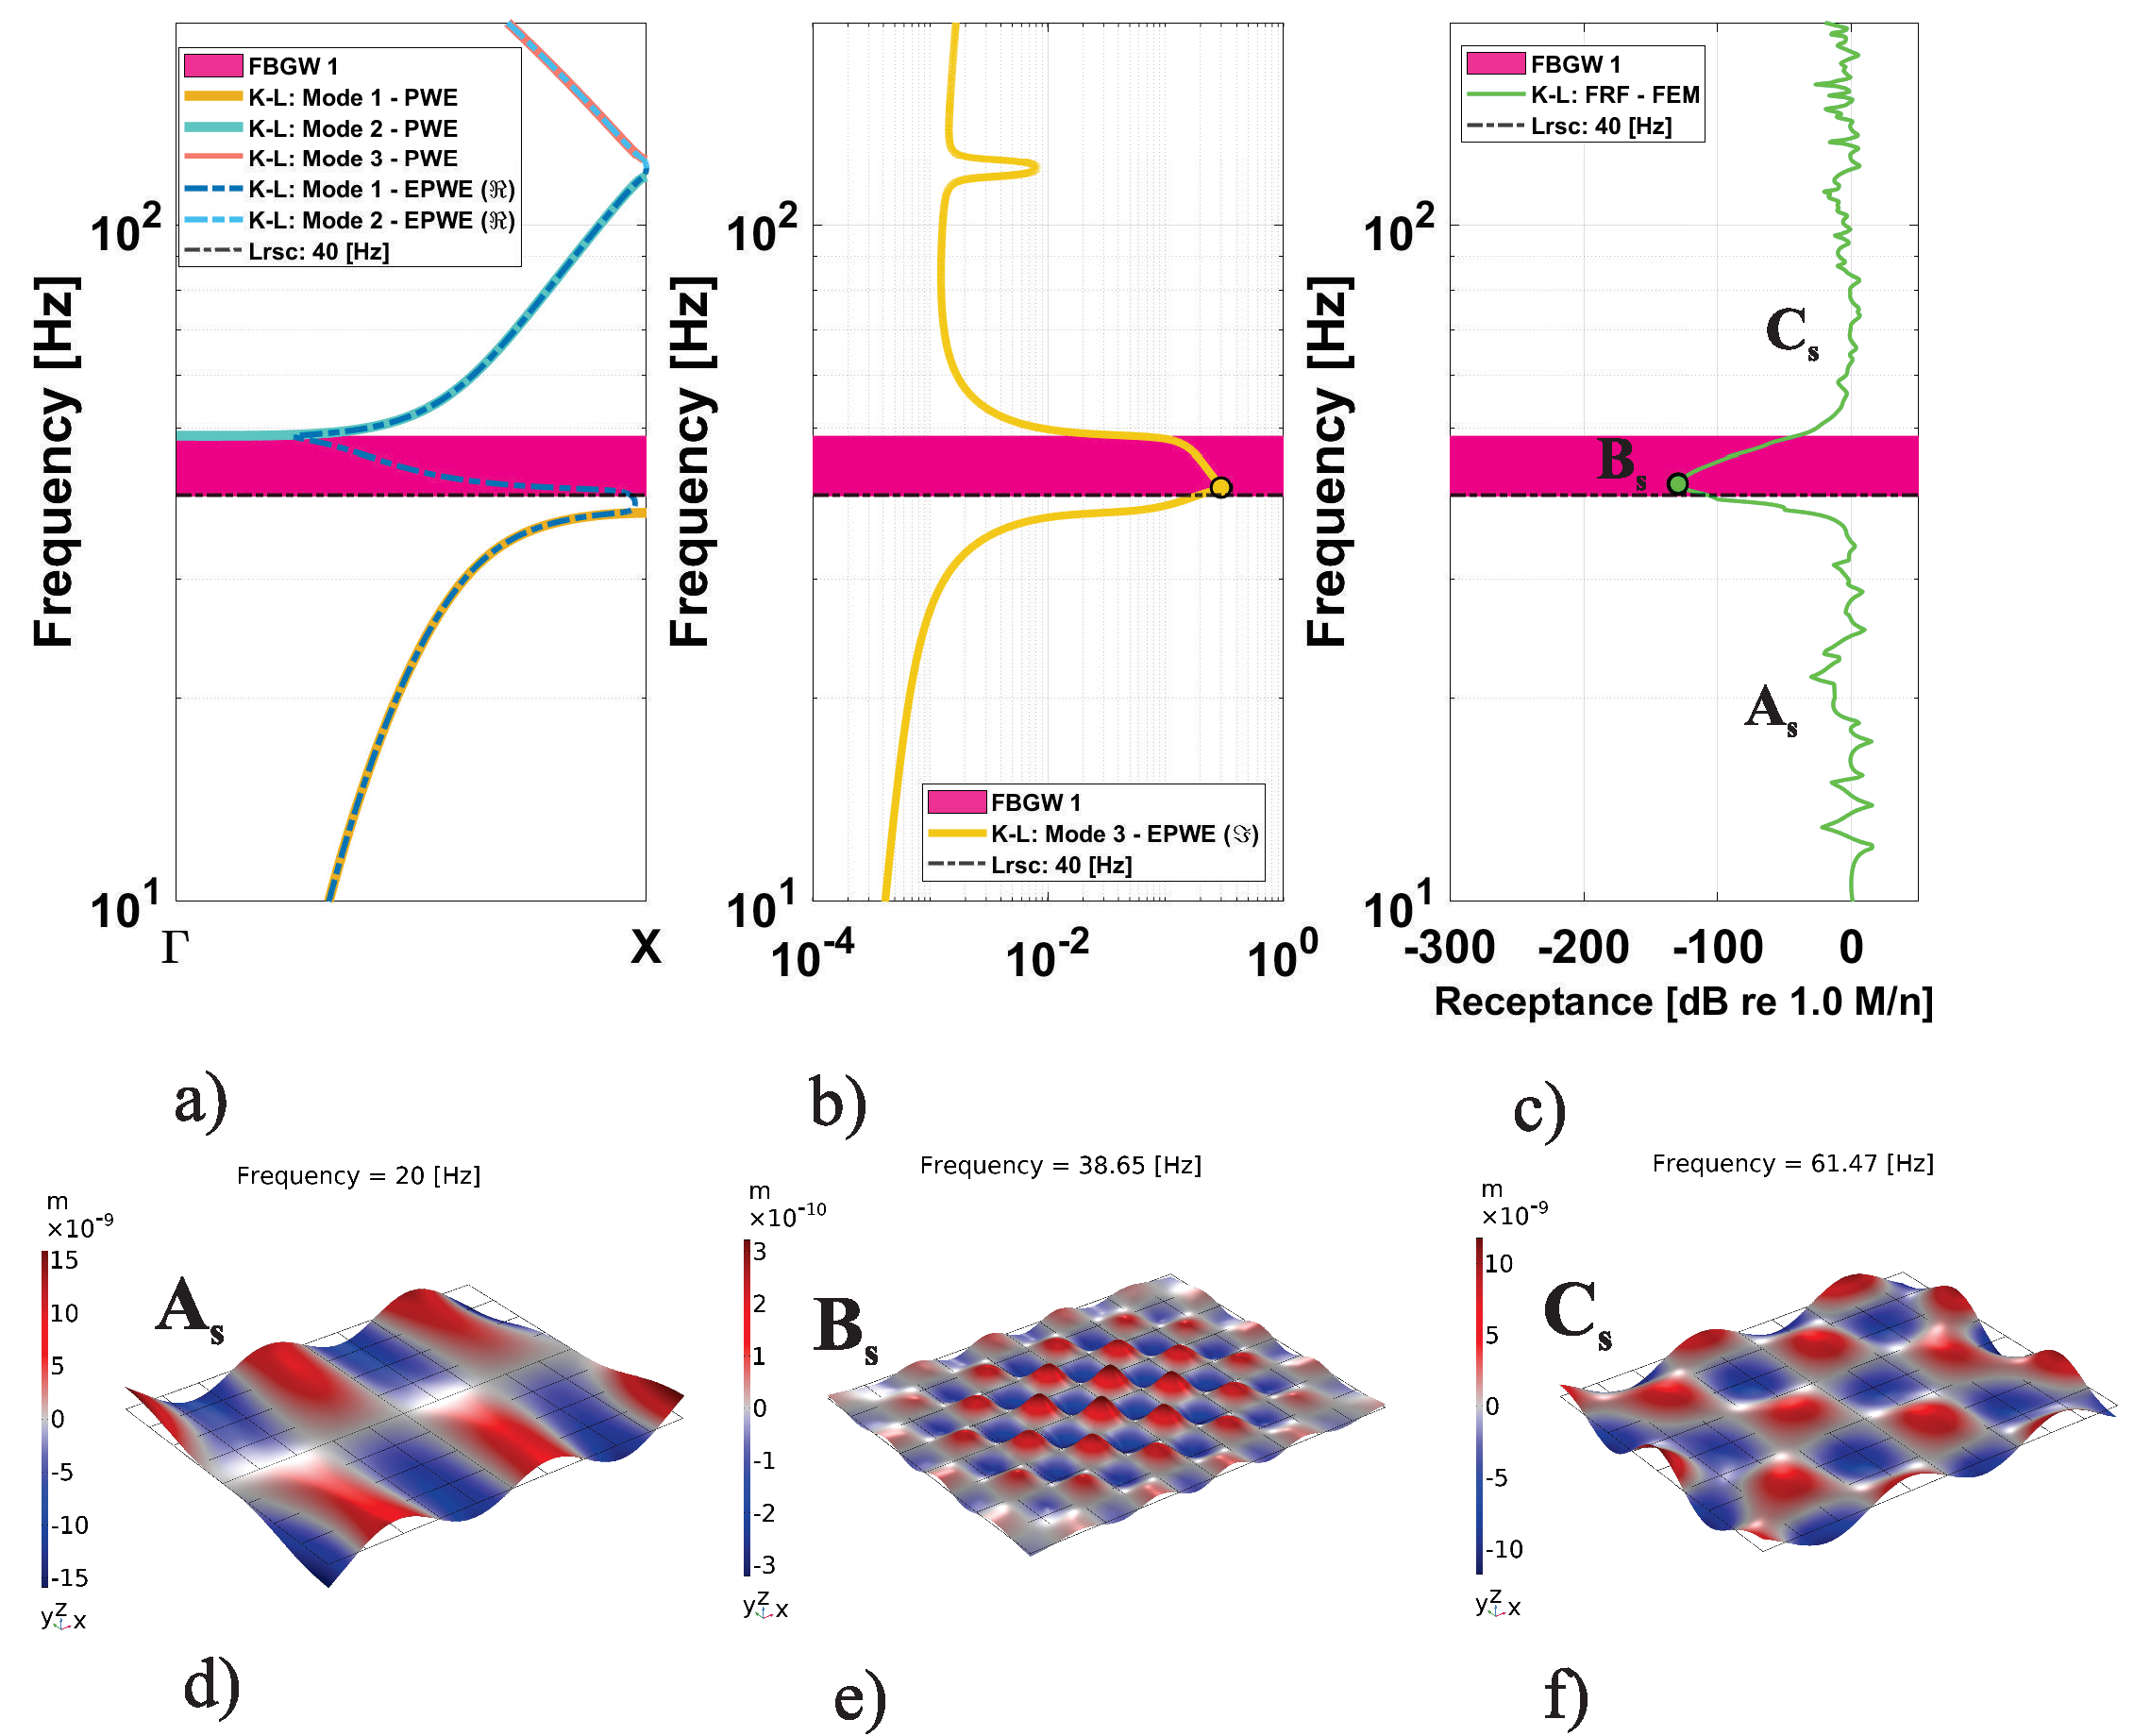
\includegraphics[width=0.8\textwidth]{1_1_disp_frf_square_pwe_epwe_recep1.pdf}
	\caption{(\textit{a}) Real band structures computed for a square unit cell with a single resonator by using PWE and real part EPWE ($\Re$). (\textit{b}) Imaginary band structures in a square unit cell with a single resonator computed by EPWE ($\Im$). (\textit{c}) Receptance computed by FEM in a LRSC panel. (\textit{d}) Vibration modes of the finite plate in a LRSC panel for frequency selection at $f_j = 20$ [Hz], (\textit{e}) $f_j = 38.65$ [Hz] and (\textit{f}) $f_j = 61.47$ [Hz].}
	\label{lat_s_pwe_epwe_tr_frf}
\end{figure}

The finite plate receptance (Figure \ref{lat_s_pwe_epwe_tr_frf}c) demonstrates excellent agreement with infinite domain predictions, achieving peak attenuation -173.09 [dB] at $f_j = 40$ [Hz]. The finite plate exhibits $50\%$ bandwidth expansion compared to theoretical FBGW 1, confirming boundary-induced mode coupling effects discussed in Section \ref{num_ex_disc}.

Figure \ref{lat_s_tr_frf_f1_f2_f3} illustrates receptance behavior across three frequency regions. Optimal performance occurs at 40 [Hz] with single peak structure, while higher frequencies (100 [Hz]) exhibit characteristic peak splitting due to modal interference between local resonators and finite plate natural frequencies.
\newpage
\begin{figure}[htb]
	\centering
	\includegraphics[width=1.0\textwidth]{2_1_disp_frf_square_3_receps.pdf}
	\caption{Vibration receptance computed by FEM in a lattice square LRSC plate (\textit{a}) in measure point  $\mathbf{u_z}$ in $f_j = 40$ [Hz], (\textit{b}) $f_j = 100$ [Hz] and (\textit{c}) $f_j = 150$ [Hz].}
	\label{lat_s_tr_frf_f1_f2_f3}
\end{figure}

The square lattice operates through single-resonator local coupling, where individual resonators interact independently with plate flexural modes. The 4-fold symmetry provides balanced coupling efficiency across orthogonal directions, making it suitable for applications requiring consistent omnidirectional performance with moderate bandwidth requirements.

The square lattice (-173.09 dB peak attenuation) serves as the fundamental reference configuration against which other geometries are compared. Its balanced 4-fold symmetry and moderate unit cell area ($A_{cell} = a^2$) represent the standard single-resonator architecture, providing the baseline for evaluating the impact of geometric modifications (rectangular anisotropy), symmetry enhancement (triangular 6-fold), and multi-resonator coupling (honeycomb, kagomé) in subsequent analyses.

\subsubsection{Rectangular lattice LRSC plate}\label{panel_lat_r}

The rectangular lattice features the smallest unit cell area $A_{cell} = a_1 \times a_2 = 0.5a^2$ with single resonator per cell ($N_j = 1$). The 2-fold symmetry creates directional anisotropy, with different propagation characteristics along orthogonal axes, resulting in a single band gap FBGW 1 between modes $f_1$ and $f_2$.

Figure \ref{lat_r_pwe_epwe_tr_frf} shows the dispersion analysis for $f_j = 40$ [Hz]. The anisotropic geometry produces directionally dependent band gaps visible in the real part (Figure \ref{lat_r_pwe_epwe_tr_frf}a), while the imaginary component (Figure \ref{lat_r_pwe_epwe_tr_frf}b) indicates reduced attenuation efficiency compared to symmetric configurations.

\begin{figure}[htb]
	\centering
	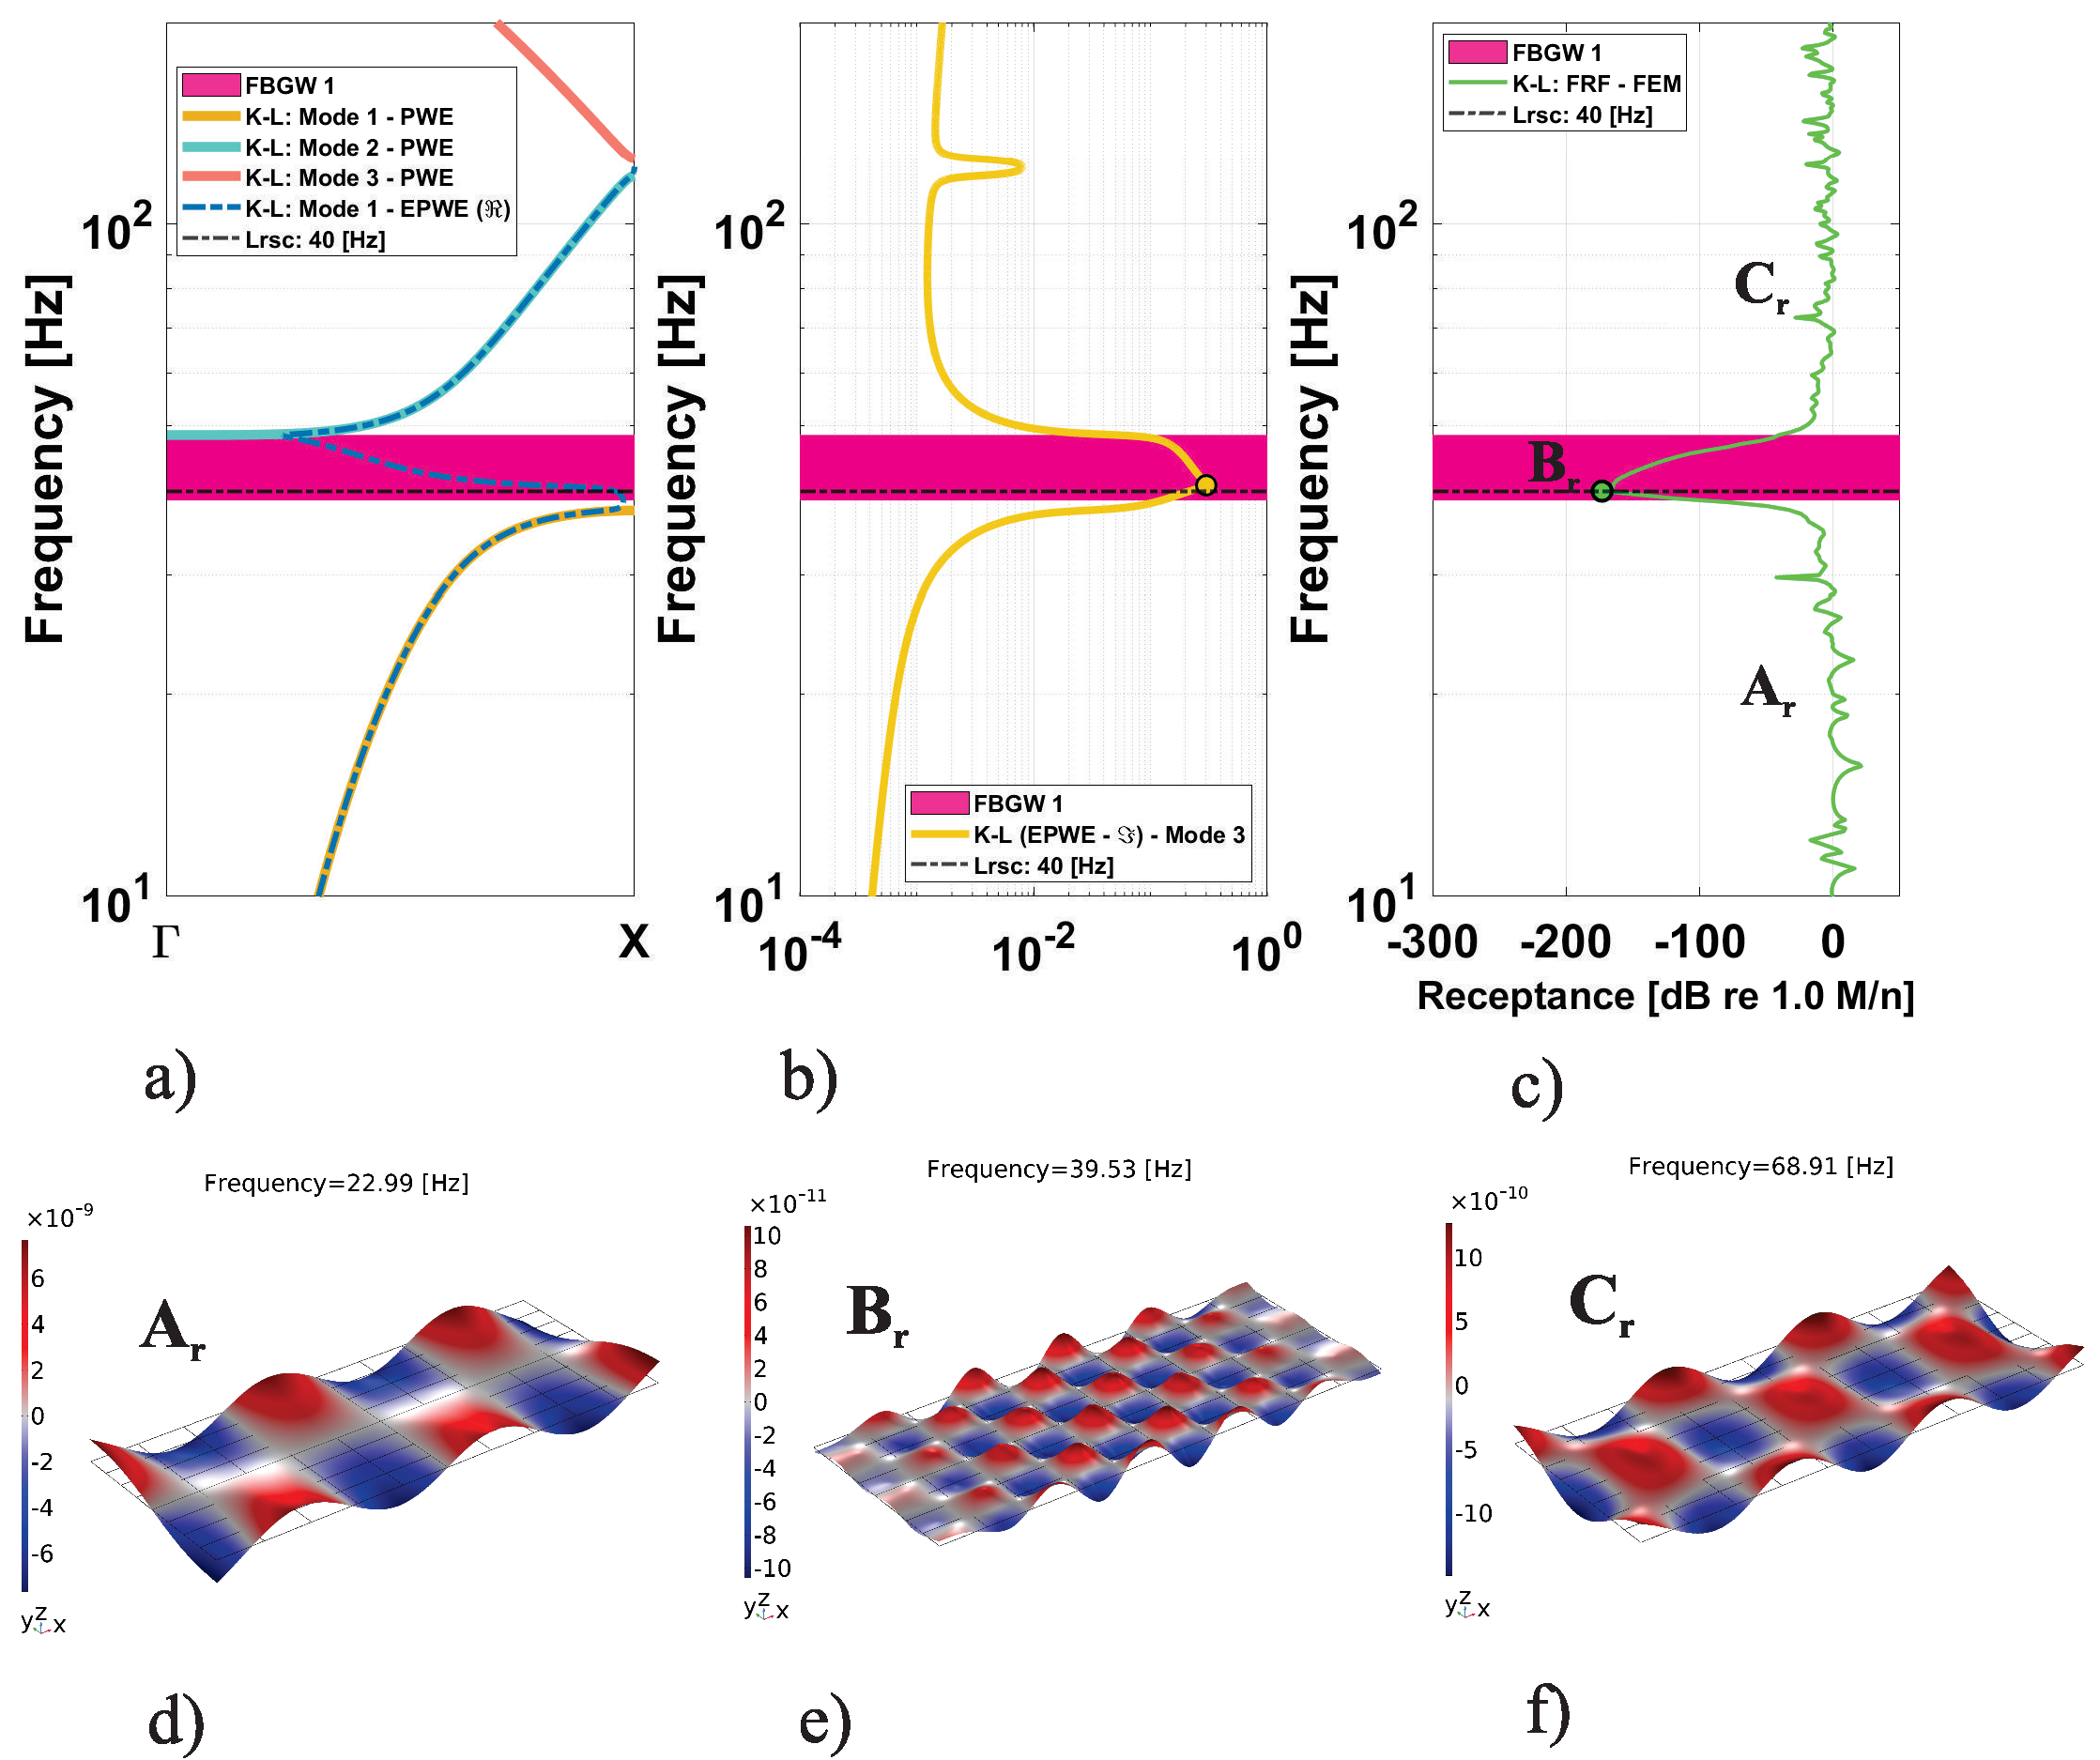
\includegraphics[width=0.8\textwidth]{1_2_disp_frf_rect_pwe_epwe_recep1.pdf}
	\caption{(\textit{a}) Real band structures computed for a rectangular unit cell with a single resonator by using PWE and real part EPWE ($\Re$). (\textit{b}) Imaginary band structures for a rectangular unit cell with a single resonator computed by EPWE ($\Im$). (\textit{c}) Receptance computed by FEM in a LRSC panel. (\textit{d}) Vibration modes of the finite plate in a LRSC panel for frequency selection at $f_j = 22.99$ [Hz], (\textit{e}) $f_j = 39.53$ [Hz] and (\textit{f}) $f_j = 68.91$ [Hz].}
	\label{lat_r_pwe_epwe_tr_frf}
\end{figure}

The finite plate receptance (Figure \ref{lat_r_pwe_epwe_tr_frf}c) achieves peak attenuation -129.93 [dB] at $f_j = 40$ [Hz], representing the lowest performance among single-resonator configurations. However, the rectangular geometry demonstrates consistent correlation with infinite domain predictions, exhibiting similar bandwidth expansion characteristics as other lattices.

Figure \ref{lat_r_tr_frf_f1_f2_f3} reveals distinctive behavior compared to symmetric lattices. The configuration maintains persistent attenuation (-80 [dB] at 177 [Hz]) even outside theoretical band gap regions, demonstrating unique resilience in finite plate applications despite limited infinite domain performance.

\begin{figure}[htb]
	\centering
	\includegraphics[width=1.0\textwidth]{2_2_disp_frf_rect_3_receps.pdf}
	\caption{Vibration receptance computed by FEM in a rectangular LRSC plate (\textit{a}) in measure point  $\mathbf{u_z}$ in $f_j = 40$ [Hz], (\textit{b}) $f_j = 90$ [Hz] and (\textit{c}) $f_j = 150$ [Hz].}
	\label{lat_r_tr_frf_f1_f2_f3}
\end{figure}

The rectangular lattice operates through constrained single-resonator coupling with directional preferences imposed by geometric anisotropy. The reduced unit cell area limits resonator-plate interaction cross-section, but creates unique finite-plate effects where boundary interactions compensate for theoretical limitations, making it suitable for space-constrained applications.

Direct comparison with the square lattice reveals the penalty of symmetry reduction: rectangular achieves -129.93 dB versus square's -173.09 [dB] ($25\%$ performance degradation). However, the geometric anisotropy creates unique advantages in finite plates, demonstrating persistent attenuation (-80 [dB] at 177 [Hz]) beyond theoretical band gaps—a phenomenon not observed in the symmetric square configuration. This establishes that while symmetry enhances peak performance, anisotropy can provide resilience in practical applications.

\subsubsection{Triangular lattice LRSC plate}\label{panel_lat_t}

The triangular lattice exhibits unit cell area $A_{cell} = a^2\sqrt{3}/2$ with single resonator per cell ($N_j = 1$). The 6-fold rotational symmetry represents the highest symmetric configuration among single-resonator lattices, creating a single broad band gap FBGW 1 between modes $f_1$ and $f_2$.

Figure \ref{lat_t_pwe_epwe_tr_frf} demonstrates the exceptional broadband characteristics for $f_j = 60$ [Hz]. The high symmetry produces the largest theoretical band gap width ($\Delta f_{12} = 55.40$ [Hz]) visible in the real part dispersion (Figure \ref{lat_t_pwe_epwe_tr_frf}a), while the imaginary component (Figure \ref{lat_t_pwe_epwe_tr_frf}b) shows superior attenuation distribution across the band gap region.

\begin{figure}[htb]
	\centering
	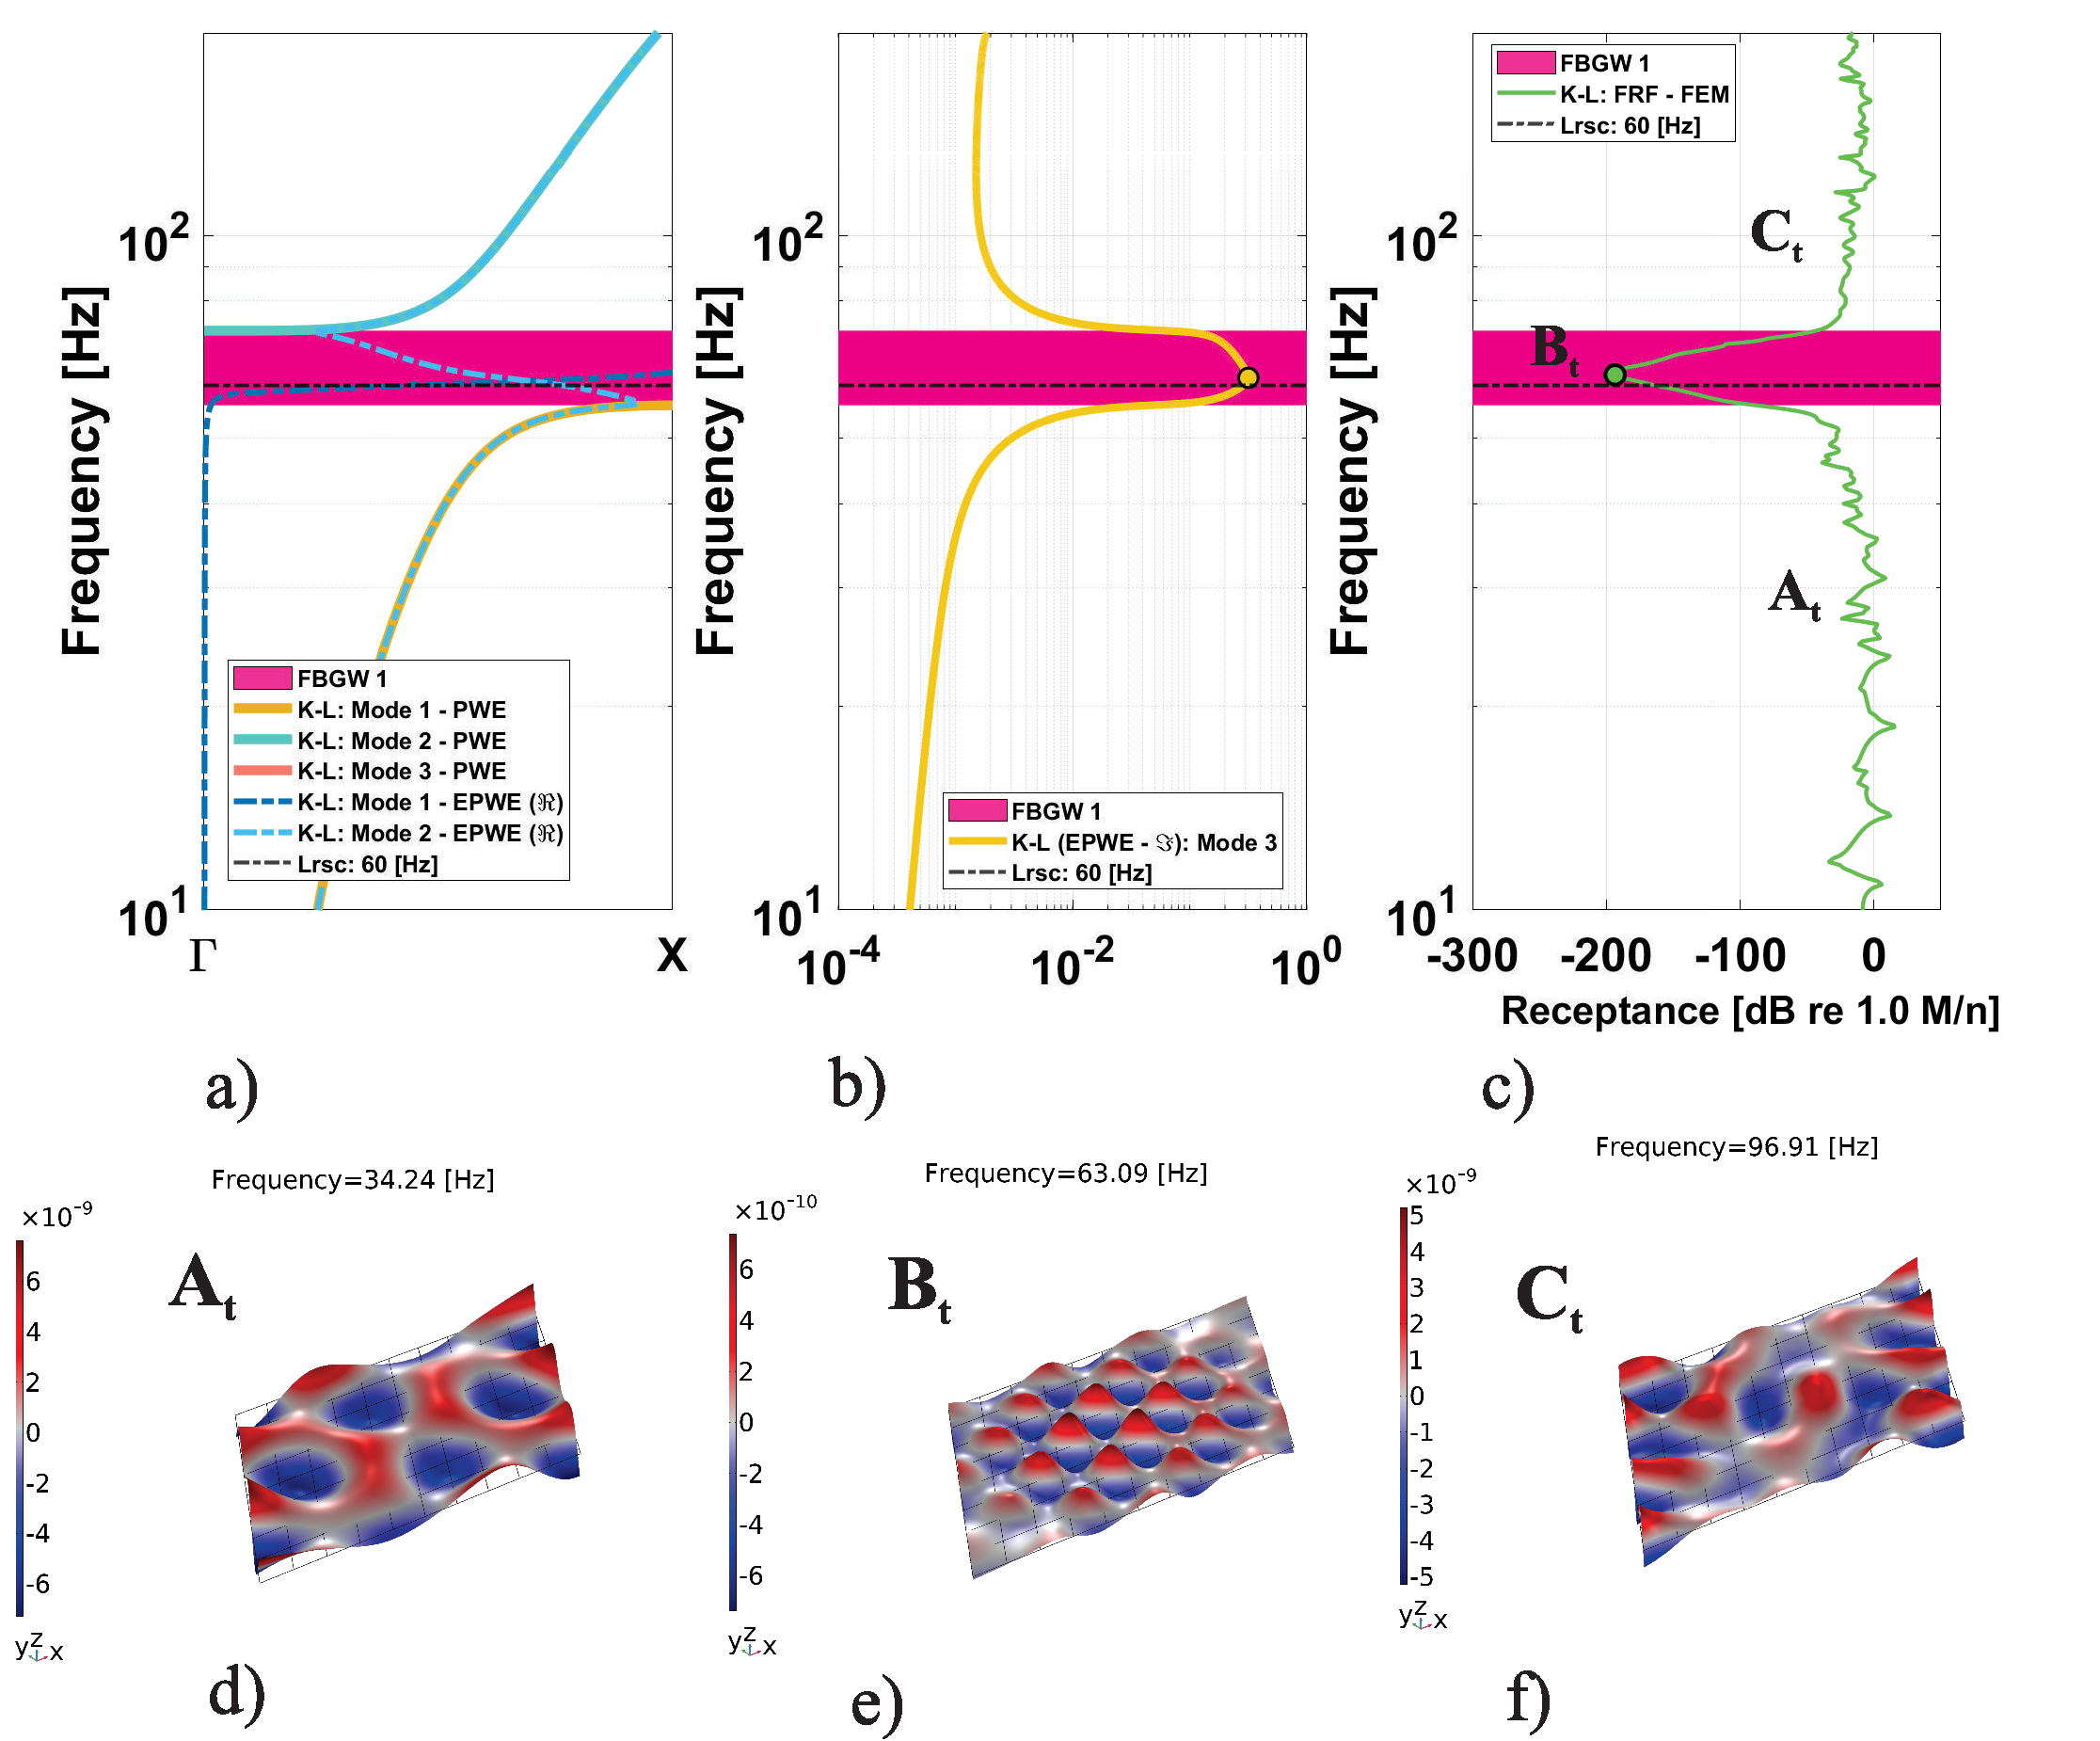
\includegraphics[width=0.8\textwidth]{1_3_disp_frf_trian_pwe_epwe_recep1.pdf}
	\caption{(\textit{a}) Real band structures computed for a triangular unit cell with a single resonator by using PWE and real part EPWE ($\Re$). (\textit{b}) Imaginary band structures for a triangular unit cell with a single resonator computed by EPWE ($\Im$). (\textit{c}) Receptance computed by FEM in a LRSC panel. (\textit{d}) Vibration modes of the finite plate in a LRSC panel for frequency selection at $f_j = 55.35$ [Hz], (\textit{e}) $f_j = 63.09$ [Hz] and (\textit{f}) $f_j = 81$ [Hz].}
	\label{lat_t_pwe_epwe_tr_frf}
\end{figure}

The finite plate receptance (Figure \ref{lat_t_pwe_epwe_tr_frf}c) achieves peak attenuation -174.19 [dB] at $f_j = 60$ [Hz], demonstrating excellent correlation with infinite domain predictions. The triangular configuration exhibits exceptional finite plate bandwidth expansion (FBGW $\approx$ 150 [Hz]), representing 43\% improvement over theoretical predictions as established in Section \ref{num_ex_disc}.

Figure \ref{lat_t_tr_frf_f1_f2_f3} illustrates the superior broadband performance across multiple frequency regions. The configuration maintains effective attenuation from 60 [Hz] through 150 [Hz], demonstrating sustained performance characteristics that validate the theoretical broadband predictions from infinite domain analysis.

\begin{figure}[htb]
	\centering
	\includegraphics[width=1.0\textwidth]{2_3_disp_frf_trian_3_receps.pdf}
	\caption{Vibration receptance computed by FEM in a triangular LRSC plate (\textit{a}) in measure point $\mathbf{u_z}$ in $f_j = 60$ [Hz], (\textit{b}) $f_j = 130$ [Hz] and (\textit{c}) $f_j = 150$ [Hz].}
	\label{lat_t_tr_frf_f1_f2_f3}
\end{figure}

The triangular lattice operates through optimized single-resonator coupling enhanced by 6-fold geometric symmetry. The high symmetry enables uniform coupling efficiency across all propagation directions, creating distributed broadband attenuation mechanisms that make it ideal for applications requiring wide-frequency vibration suppression with moderate peak attenuation requirements.

The triangular lattice demonstrates the optimal single-resonator configuration, achieving -174.19 [dB] peak attenuation ($0.6\%$ improvement over square, $34\%$ over rectangular) with exceptional bandwidth expansion (FBGW $\approx$ 150 [Hz]). Compared to previous configurations: (i) $4\%$ performance increase over square baseline; (ii) $34\%$ advantage over rectangular; (iii) superior broadband characteristics validate Section \ref{num_ex_disc} predictions. The high symmetry establishes the performance ceiling for single-resonator architectures, setting expectations for multi-resonator systems.

\subsubsection{Honeycomb lattice LRSC plate}\label{panel_lat_h}

The honeycomb lattice features unit cell area $A_{cell} = 3a^2\sqrt{3}/2$ with dual resonators per cell ($N_j = 2$). This configuration exhibits 6-fold symmetry while introducing inter-resonator coupling mechanisms, creating two potential band gaps: FBGW 1 between modes $f_2$ and $f_3$, and FBGW 2 between modes $f_3$ and $f_4$.

Figure \ref{lat_h_pwe_epwe_tr_frf} illustrates the dual-resonator dynamics for $f_j = 30$ [Hz]. The real part dispersion (Figure \ref{lat_h_pwe_epwe_tr_frf}a) reveals multiple band gap regions, while the imaginary component (Figure \ref{lat_h_pwe_epwe_tr_frf}b) shows enhanced attenuation peaks corresponding to synchronized dual-resonator oscillations within both FBGW 1 and FBGW 2 regions.
\newpage
\begin{figure}[htb]
	\centering
	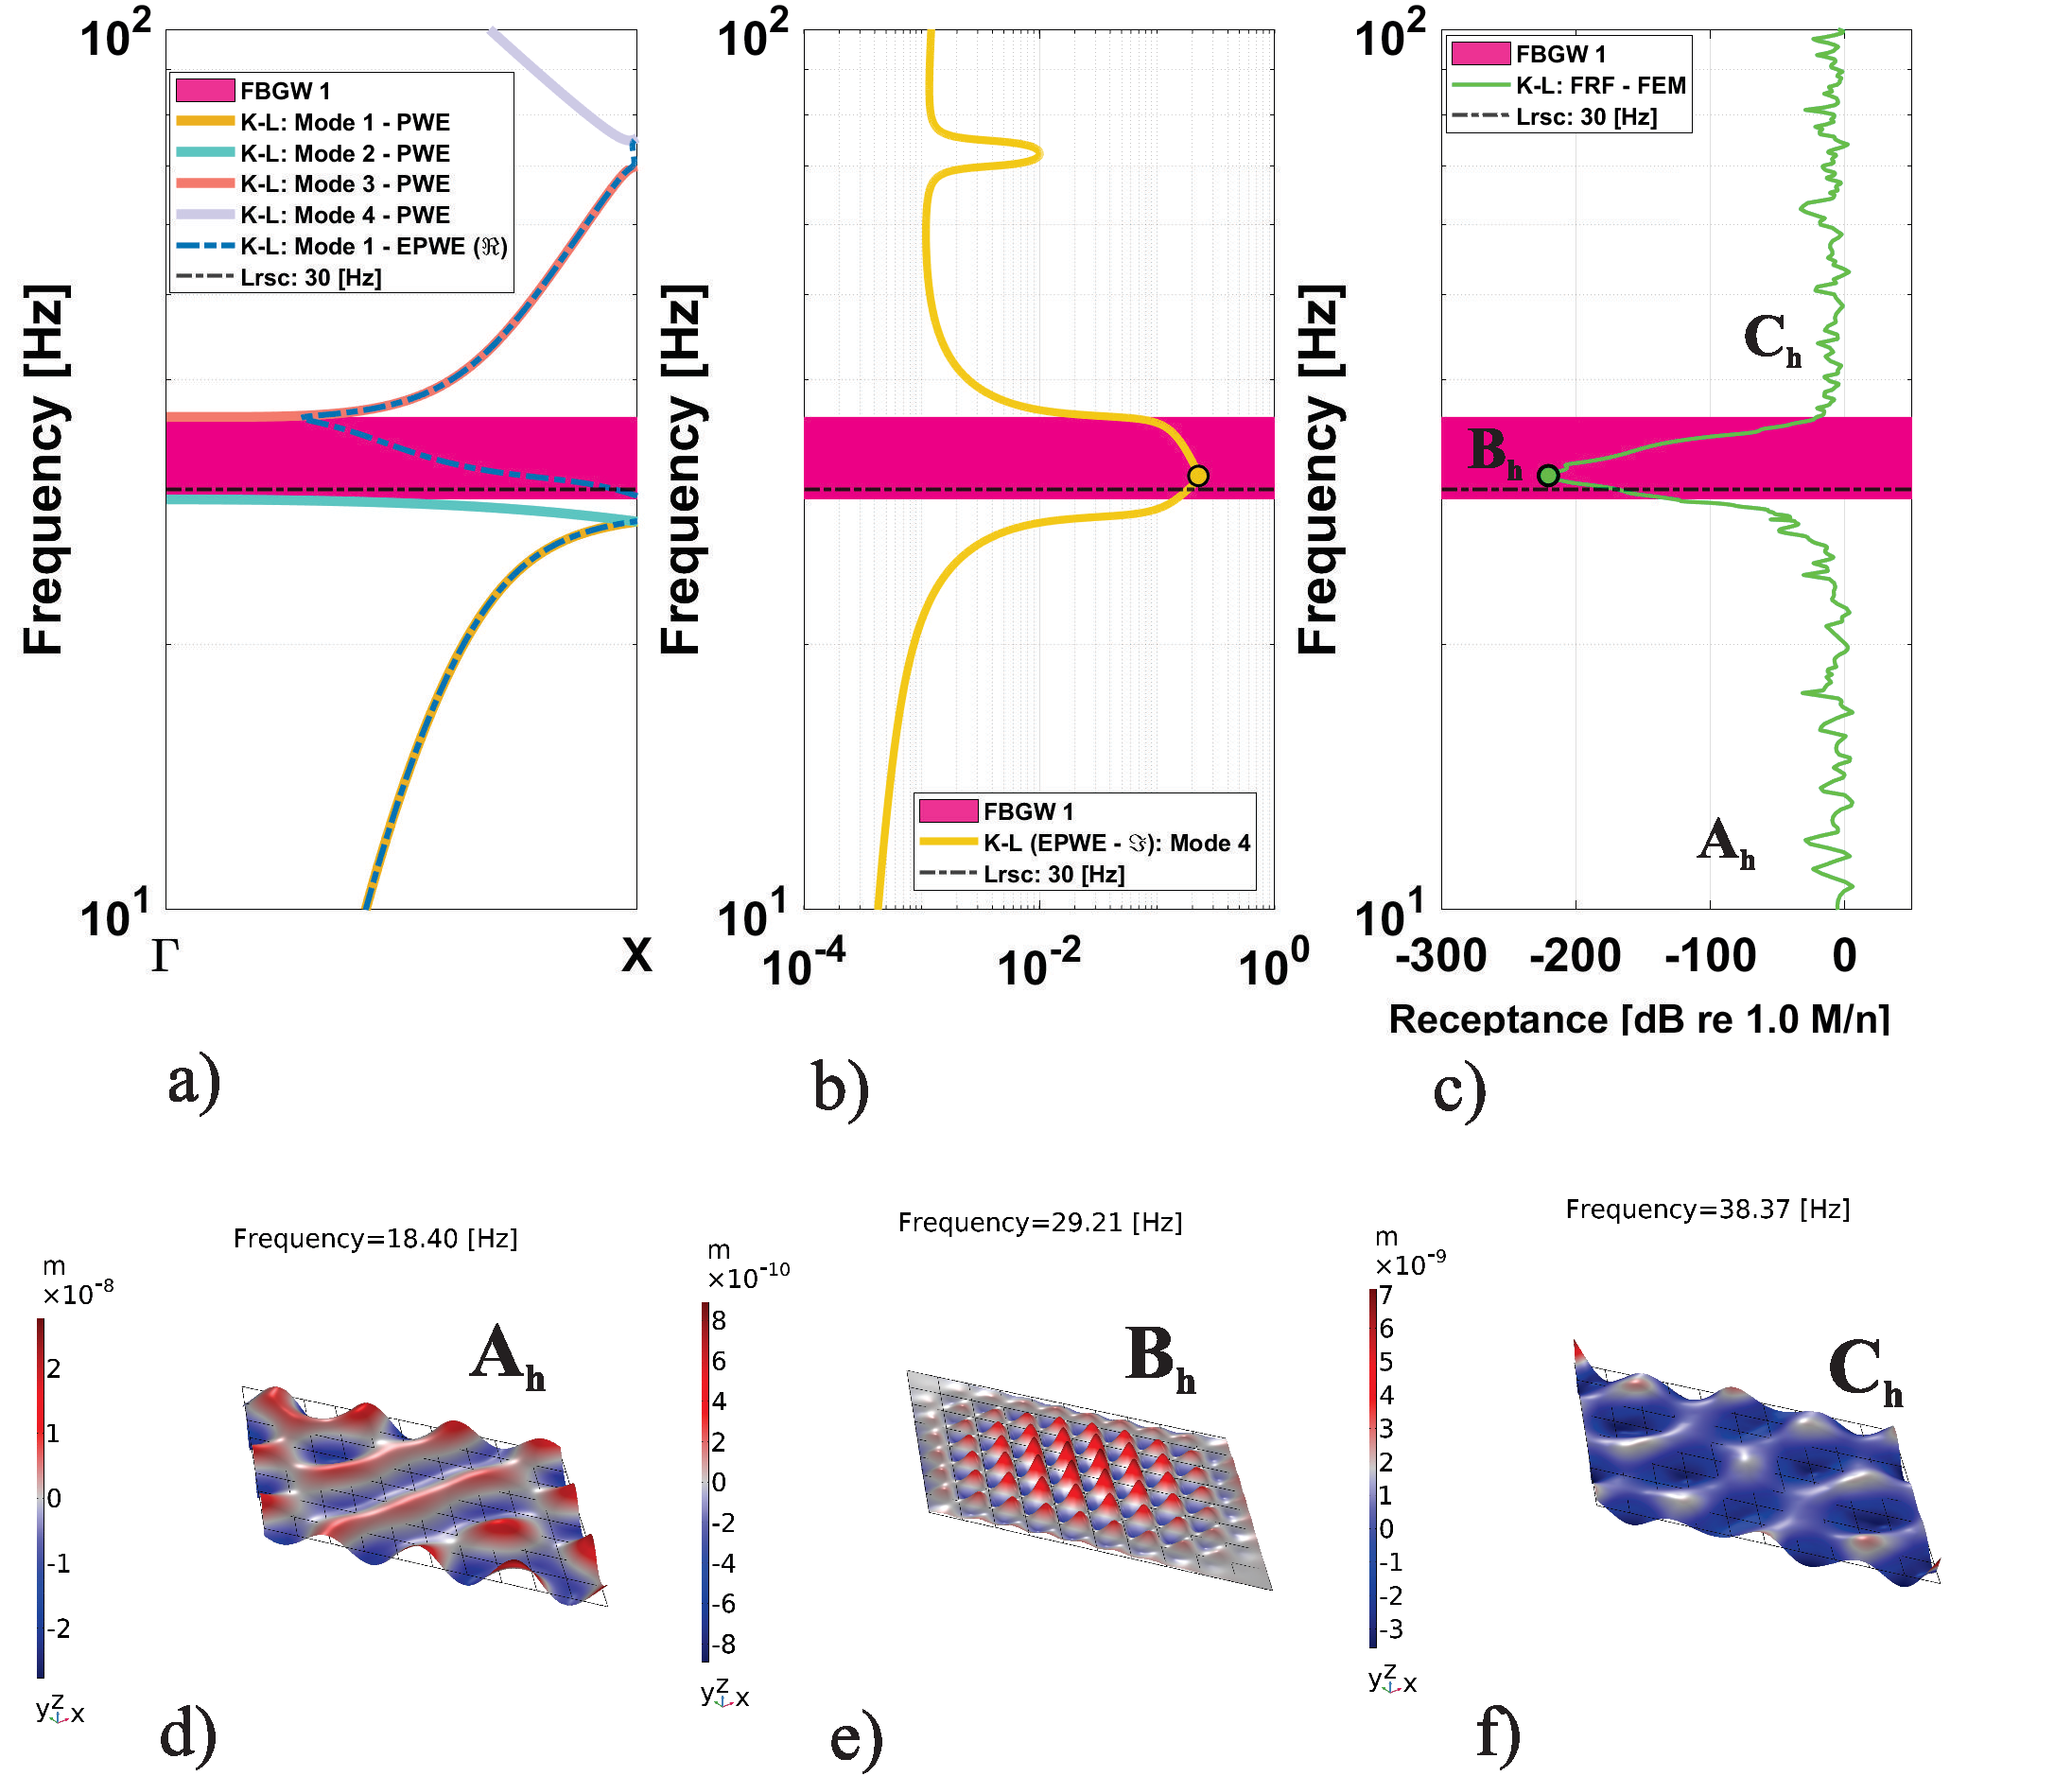
\includegraphics[width=0.8\textwidth]{1_4_disp_frf_hex_pwe_epwe_recep1.pdf}
	\caption{(\textit{a}) Real band structures computed for a honeycomb unit cell with two resonators by using PWE and real part EPWE ($\Re$). (\textit{b}) Imaginary band structures for a honeycomb unit cell with two resonators computed by EPWE ($\Im$). (\textit{c}) Receptance computed by FEM in a LRSC panel. (\textit{d}) Vibration modes of the finite plate in a LRSC panel for frequency selection at $f_j = 18.40$ [Hz], (\textit{e}) $f_j = 29.21$ [Hz] and (\textit{f}) $f_j = 38.37$ [Hz].}
	\label{lat_h_pwe_epwe_tr_frf}
\end{figure}

The finite plate receptance (Figure \ref{lat_h_pwe_epwe_tr_frf}c) achieves peak attenuation -220.33 [dB] at $f_j = 30$ [Hz], demonstrating superior performance compared to single-resonator configurations. The dual-resonator coupling creates enhanced local impedance mismatch, resulting in stronger wave scattering and improved finite plate correlation with infinite domain predictions.

Figure \ref{lat_h_tr_frf_f1_f2_f3} demonstrates the unique capability of coexisting band gaps. At specific frequencies ($f_j = 50$ [Hz]), both FBGW 1 and FBGW 2 contribute to attenuation, expanding the effective bandwidth. The dual-resonator system exhibits sustained performance across multiple frequency regions, validating the multi-band gap theoretical predictions.
\newpage
\begin{figure}[htb]
	\centering
	\includegraphics[width=1.0\textwidth]{2_4_disp_frf_hex_3_receps.pdf}
	\caption{Vibration receptance computed by FEM in a LRSC plate (\textit{a}) in measure point $\mathbf{u_z}$  for $f_j = 30$ [Hz], (\textit{b}) $f_j = 50$ [Hz] and (\textit{c}) $f_j = 150$ [Hz].}
	\label{lat_h_tr_frf_f1_f2_f3}
\end{figure}

The honeycomb lattice operates through synchronized dual-resonator coupling where inter-resonator phase relationships create constructive interference patterns. The two resonators within each unit cell exhibit coordinated motion that doubles the local impedance mismatch, enabling superior energy extraction from plate flexural modes. This configuration provides balanced performance between peak attenuation and bandwidth coverage, making it suitable for applications requiring both high attenuation and moderate broadband characteristics.

The honeycomb lattice (-220.33 [dB]) establishes the first significant performance jump from single-resonator configurations, achieving $27\%$ improvement over triangular (current single-resonator leader) and $70\%$ over rectangular. The dual-resonator coupling creates: (i) 46.14 [dB] advantage over best single-resonator (triangular); (ii) coexisting dual band gaps unavailable in single-resonator systems; (iii) validation of inter-resonator coupling theory from Section \ref{num_ex_disc}. This confirms that resonator multiplication, when properly configured, provides substantial benefits beyond geometric optimization alone.

\subsubsection{Kagomé lattice LRSC plate}\label{panel_lat_k}

The kagomé lattice exhibits the largest unit cell area $A_{cell} = 2a^2\sqrt{3}$ with triple resonators per cell ($N_j = 3$). The three resonators positioned at 120° intervals create complex multi-resonator coupling mechanisms, generating two potential band gaps: FBGW 1 between modes $f_3$ and $f_4$, and FBGW 2 between modes $f_5$ and $f_6$.

Figure \ref{lat_k_pwe_epwe_tr_frf} demonstrates the exceptional triple-resonator dynamics for $f_j = 20$ [Hz]. The real part dispersion (Figure \ref{lat_k_pwe_epwe_tr_frf}a) reveals narrow but well-defined band gaps, while the imaginary component (Figure \ref{lat_k_pwe_epwe_tr_frf}b) shows maximum attenuation peaks corresponding to synchronized triple-resonator oscillations, creating the highest attenuation among all configurations.

\begin{figure}[htb]
	\centering
	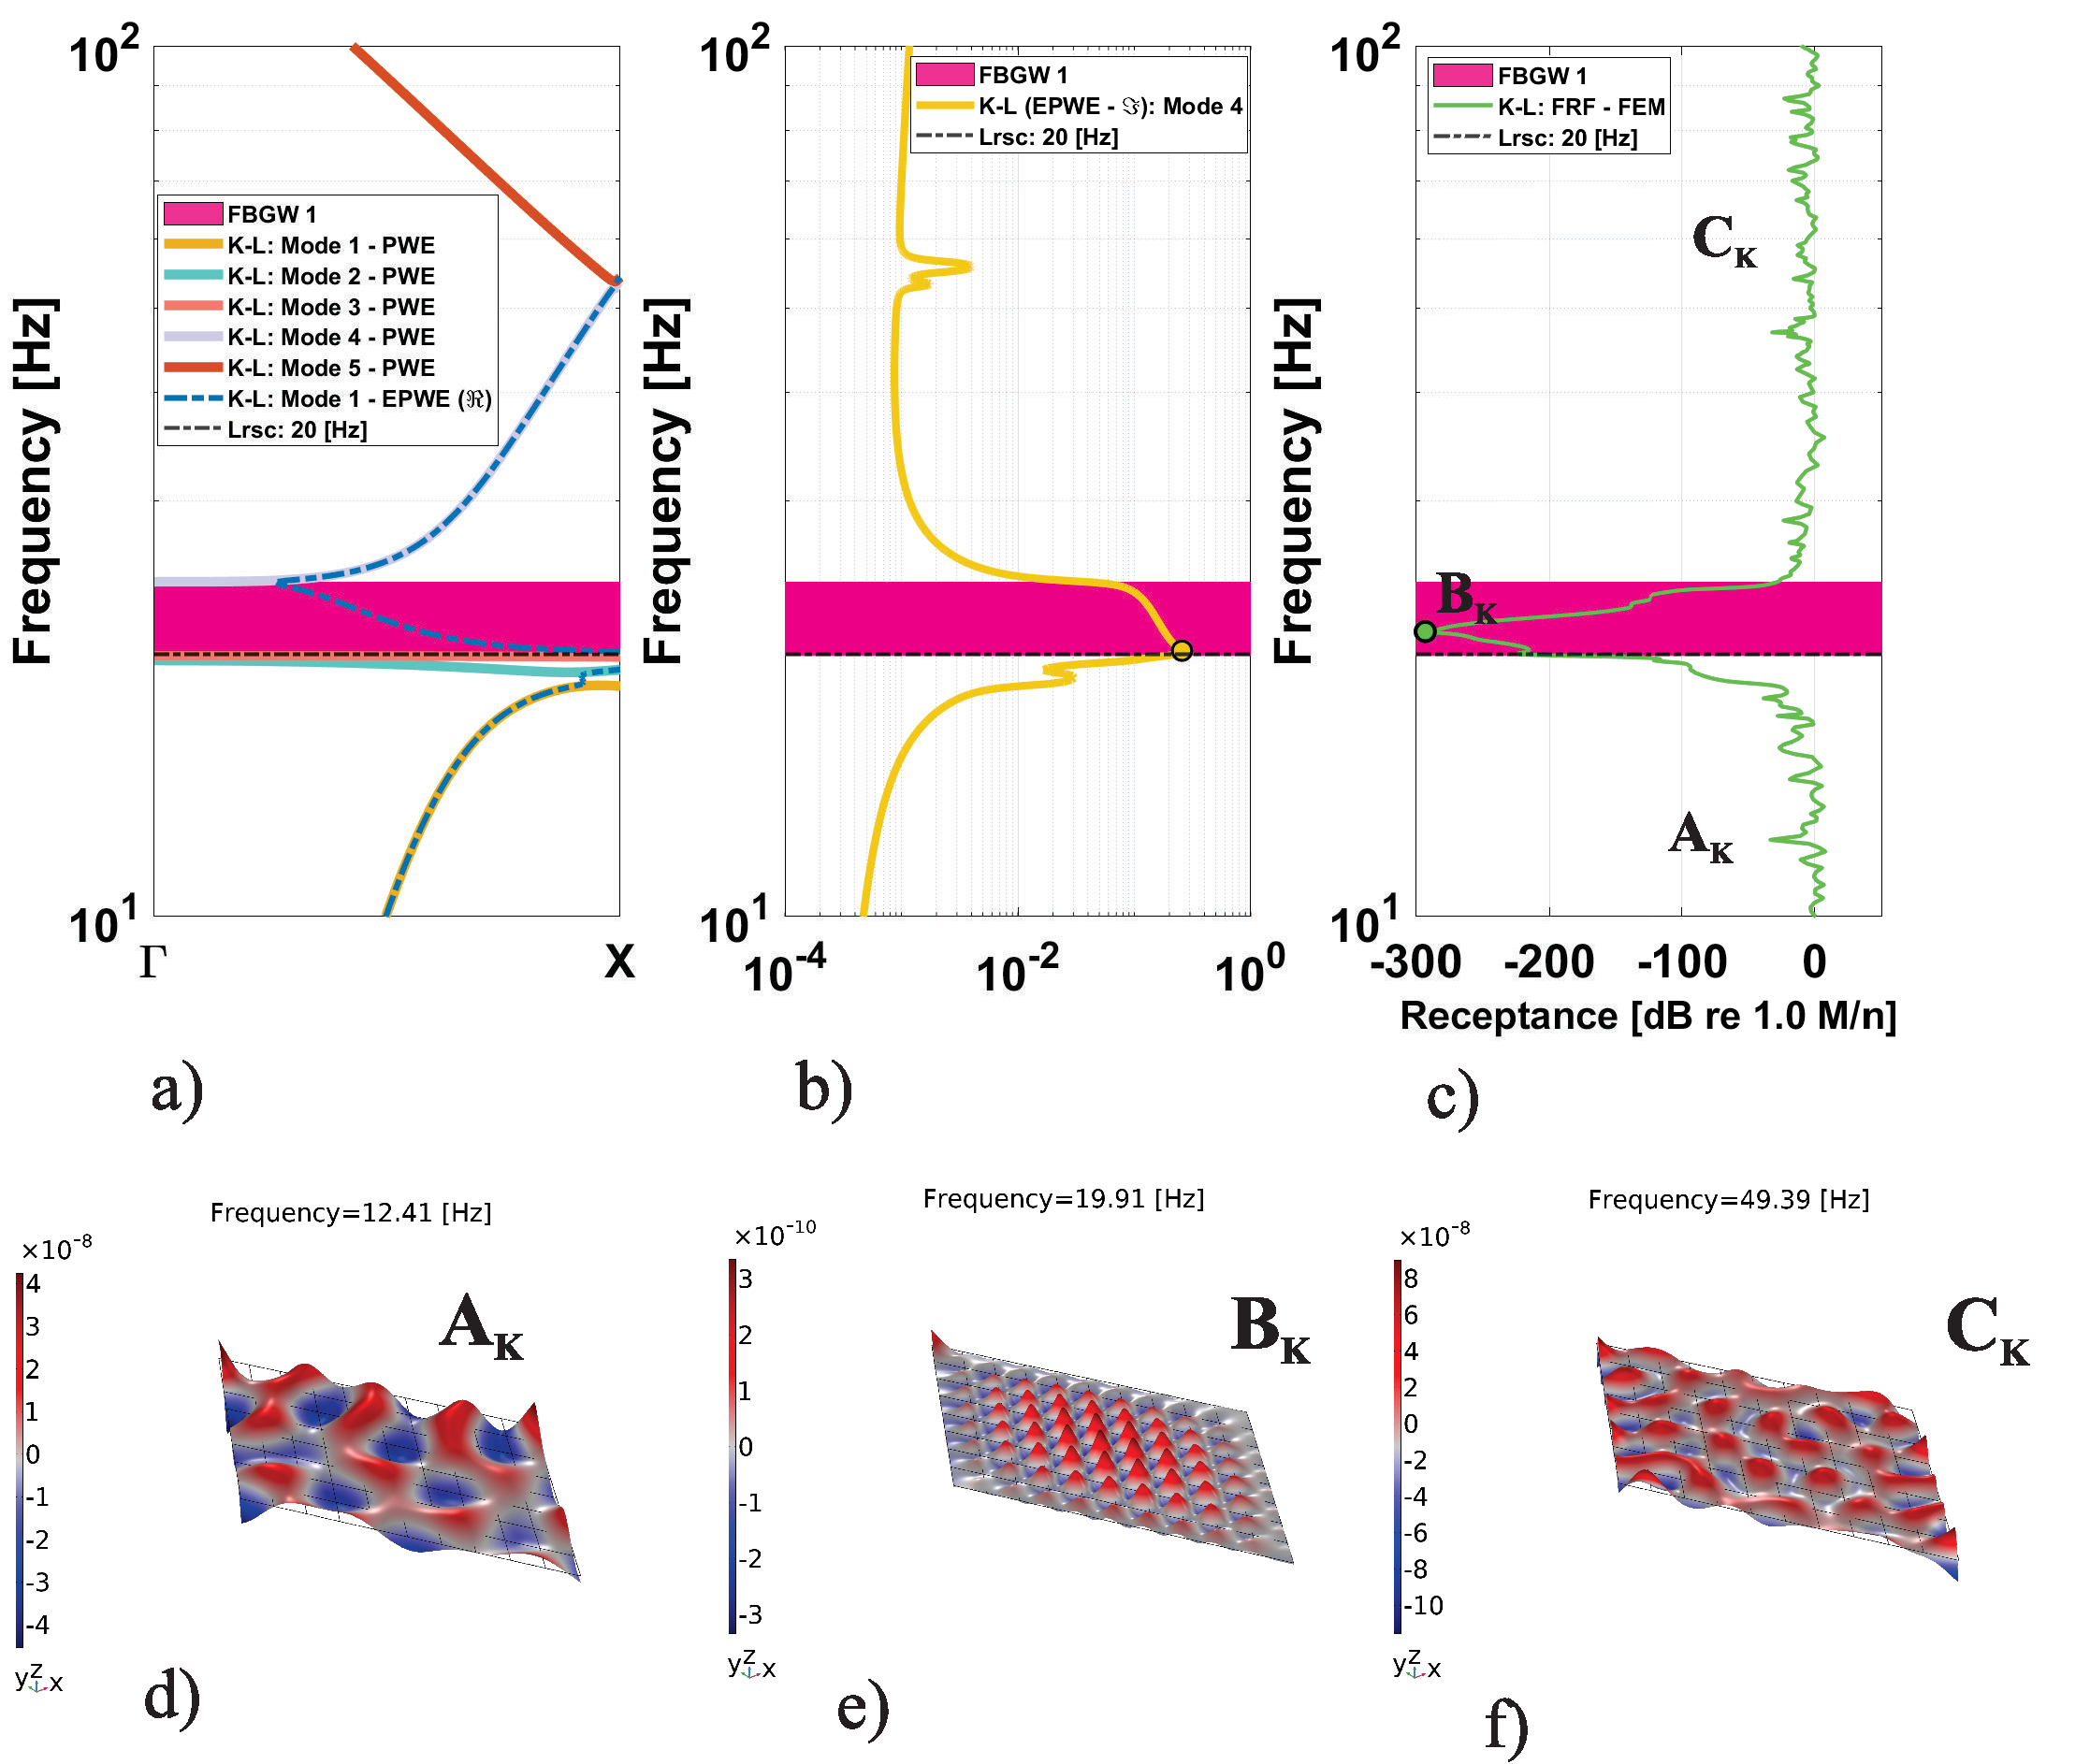
\includegraphics[width=0.8\textwidth]{1_5_disp_frf_kag_pwe_epwe_recep1.pdf}
	\caption{(\textit{a}) Real band structures computed for a kagomé unit cell with three resonators by using PWE and real part EPWE ($\Re$). (\textit{b}) Imaginary band structures for a kagomé unit cell with three resonators computed by EPWE ($\Im$). (\textit{c}) Receptance computed by FEM in a LRSC panel. (\textit{d}) Vibration modes of the finite plate in a LRSC panel for frequency selection at $f_j = 12.41$ [Hz], (\textit{e}) $f_j = 19.91$ [Hz] and (\textit{f}) $f_j = 49.39$ [Hz].}
	\label{lat_k_pwe_epwe_tr_frf}
\end{figure}

The finite plate receptance (Figure \ref{lat_k_pwe_epwe_tr_frf}c) achieves extraordinary peak attenuation -292.65 [dB] at $f_j = 20$ [Hz], representing the highest performance among all analyzed configurations. The triple-resonator coupling creates localized energy concentration through constructive interference patterns, demonstrating exceptional correlation between collective resonator impedance mismatch and finite plate attenuation.

Figure \ref{lat_k_tr_frf_f1_f2_f3} illustrates the comprehensive attenuation behavior across multiple frequency regions. The kagomé configuration exhibits frequency-selective characteristics with maximum effectiveness at low frequencies, while maintaining the capability for dual band gap coexistence at specific resonator tunings ($f_j = 60$ [Hz]), validating the multi-resonator theoretical framework.

\begin{figure}[htb]
	\centering
	\includegraphics[width=1.0\textwidth]{2_5_disp_frf_kag_3_receps.pdf}
	\caption{Vibration receptance computed by FEM in a LRSC plate (\textit{a)}) in measure point $\mathbf{u_z}$  for $f_j = 20$ [Hz], (\textit{b)}) $f_j = 60$ [Hz] and (\textit{c)}) $f_j = 150$ [Hz].}
	\label{lat_k_tr_frf_f1_f2_f3}
\end{figure}

The kagomé lattice operates through synchronized triple-resonator coupling where three resonators at 120° intervals create complex phase relationships optimized for triangular symmetry. This multi-resonator arrangement generates localized energy concentration through constructive interference patterns, where each resonator contributes to collective impedance mismatch that far exceeds individual contributions. The configuration provides extraordinary frequency-selective energy dissipation, making it ideal for applications requiring maximum attenuation at specific target frequencies.

The kagomé lattice (-292.65 [dB]) represents the performance apex, demonstrating $33\%$ improvement over honeycomb and $68\%$ over triangular configurations. Progressive performance escalation confirms design principles: rectangular (-129.93 [dB]) < square (-173.09 [dB]) < triangular (-174.19 [dB]) < honeycomb (-220.33 [dB]) < kagomé (-292.65 [dB]). The 162.72 [dB] span between worst (rectangular) and best (kagomé) validates both geometric optimization and resonator multiplication strategies, establishing clear design guidelines for target-specific applications.

Individual analysis reveals three fundamental design strategies: (i) Geometric optimization (rectangular → square → triangular) provides moderate improvements through symmetry enhancement; (ii) Multi-resonator coupling (single → dual → triple) creates substantial performance jumps through synchronized oscillations; (iii) Application-specific selection requires balancing peak attenuation (kagomé), broadband performance (triangular), and dual-mode capability (honeycomb). The counterintuitive finding that local resonator-plate coupling dominates over global wave interference, with finite plates exhibiting consistent $40-50\%$ bandwidth expansion, establishes fundamental principles for metamaterial plate design.

After analyzing each of the five panels with different periodic lattices individually, the next subsection presents a comparative analysis of attenuation performance across three frequency ranges, providing a broader understanding of the obtained results. A comprehensive framework for practical lattice selection in engineering applications is provided in Appendix D.

%%%%%%%%%%%%%%%%%%%%%%%
\subsection{Analysis comparative with all LRSC plates}\label{comp_panels_all_lats}
After discussing the primary attenuation characteristics of receptance for each of the five periodic lattice plates individually---emphasizing key aspects across the entire frequency range of their local resonators---this final subsection focuses on a comparative analysis of the receptance attenuation performance among these plates. To manage the data effectively, this study divides the resonance frequencies into three regions: Region 1 ($10$ to $50$ [Hz]), Region 2 ($60$ to $100$ [Hz]), and Region 3 ($110$ to $150$ [Hz]). The comparative analysis of lattice geometries and their impact on wave propagation builds upon the work of \cite{Yan2022}, who investigated metamaterial plates with various lattices for low-frequency vibration attenuation.
Figure \ref{all_comp_frf_stat_lat} presents boxplots for these regions, individually summarizing the statistical characteristics of the attenuation performance for each of the five lattices, as illustrated:
\newpage
\begin{figure}[htb]
	\centering	
	\includegraphics[width=1.0\textwidth]{all_comp_frf_stat_lat.pdf}	
	\caption{Descriptive statistical analysis for the five lattice panel types at measurement point $\mathbf{u_z}$: \textit{a)} Region 1, $f_j = 10$ -- $50$ [Hz]; \textit{b)} Region 2, $f_j = 60$ -- $100$ [Hz]; \textit{c)} Region 3, $f_j = 110$ -- $150$ [Hz].}
	\label{all_comp_frf_stat_lat}
\end{figure}

The statistical analysis reveals distinct performance characteristics across three frequency regions: Region 1 (10-50 [Hz]) dominated by kagomé peak performance (-292.65 [dB]) and honeycomb consistency; Region 2 (60-100 [Hz]) showing triangular and honeycomb FBGW 2 optimization; Region 3 (110-150 [Hz]) demonstrating triangular broadband superiority. The key findings from the statistical analysis are summarized in Table \ref{tab_tr_lattices_10_50}:
\newpage
\begin{table}[htb]
    \centering
\caption{Receptance attenuation results of $\mathbf{R_z}$ for different lattice configurations: \( s \) (Square), \( r \) (Rectangular), \( t \) (Triangular), \( h_1 \) and \( h_2 \) (Honeycomb for FBGW 1 and 2), \( k_1 \) and \( k_2 \) (Kagomé for FBGW 1 and 2), in the frequency range of 10 to 50 [Hz].}

    \begin{tabular}{cccccccc}
        $f_j$ [Hz] & $s$  [dB] & $r$  [dB] & $t$  [dB] & $h_1$ [dB] & $h_2$ [dB] & $k_1$ [dB] & $k_2$ [dB] \\ \hline
        10         & -91.92            & -77.69                  & -97.60                & -185.09                & -3.89                  & -260.51               & -3.68                \\ \hline
        20         & -128.51           & -105.98                 & -133.41               & -217.34                & -12.62                 & -292.65               & -6.15                \\ \hline
        30         & -150.05           & -122.46                 & -157.86               & -220.33                & -11.61                 & -211.26               & -14.95               \\ \hline
        40         & -173.09           & -129.93                 & -174.19               & -201.55                & -20.06                 & -183.08               & -47.64               \\ \hline
        50         & -162.33           & -129.51                 & -158.97               & -155.43                & -64.28                 & -100.28               & -96.81               \\ \hline
    \end{tabular}
    \label{tab_tr_lattices_10_50}
\end{table}

Detailed results for Regions 2 and 3 are presented in Tables \ref{tab_tr_lattices_60_100} and \ref{tab_tr_lattices_110_150}:

\begin{table}[htb]
    \centering
    \caption{Receptance attenuation results of $\mathbf{R_z}$ for different lattice configurations: \( s \) (Square), \( r \) (Rectangular), \( t \) (Triangular), \( h_1 \) and \( h_2 \) (Honeycomb for FBGW 1 and 2), \( k_1 \) and \( k_2 \) (Kagomé for FBGW 1 and 2), in the frequency range of 60 to 100 [Hz].}
    \begin{tabular}{cccccccc}
        $f_j$ [Hz] & $s$  [dB] & $r$  [dB] & $t$  [dB] & $h_1$ [dB] & $h_2$ [dB] & $k_1$ [dB] & $k_2$ [dB] \\ \hline
        60         & -141.16           & -119.82                 & -193.44               & -83.41                & -119.60                 & -100.70               & -96.11                \\ \hline
        70         & -115.75           & -104.04                 & -191.36               & -54.46                & -148.16                 & -98.53                & -157.24               \\ \hline
        80         & -105.40           & -107.52                 & -154.46               & -15.87                & -153.16                 & -111.48               & -198.27               \\ \hline
        90         & -88.22            & -121.26                 & -134.05               & -7.37                 & -163.82                 & -79.85                & -143.85               \\ \hline
        100        & -72.01            & -84.52                  & -116.57               & -28.36                & -165.83                 & -48.78                & -159.56               \\ \hline
    \end{tabular}
    \label{tab_tr_lattices_60_100}
\end{table}
\newpage
\begin{table}[htb]
    \centering
    \caption{Receptance attenuation results of $\mathbf{R_z}$ for different lattice configurations: \( s \) (Square), \( r \) (Rectangular), \( t \) (Triangular), \( h_1 \) and \( h_2 \) (Honeycomb for FBGW 1 and 2), \( k_1 \) and \( k_2 \) (Kagomé for FBGW 1 and 2), in the frequency range of 110 to 150 [Hz].}
    \begin{tabular}{cccccccc}
        $f_j$ [Hz] & $s$  [dB] & $r$  [dB] & $t$  [dB] & $h_1$ [dB] & $h_2$ [dB] & $k_1$ [dB] & $k_2$ [dB] \\ \hline
        110        & -21.26            & -89.71                  & -123.67               & -7.77                & -163.06                 & -34.55                & -171.89               \\ \hline
        120        & -20.89            & -86.18                  & -119.74               & -5.56                & -161.97                 & -25.93                & -165.01               \\ \hline
        130        & -20.33            & -73.31                  & -106.28               & -4.59                & -150.43                 & -21.48                & -148.52               \\ \hline
        140        & -19.71            & -68.05                  & -99.32                & -4.57                & -140.96                 & -18.78                & -139.51               \\ \hline
        150        & -18.94            & -65.58                  & -95.31                & -3.45                & -132.93                 & -14.57                & -130.71               \\ \hline
    \end{tabular}
    \label{tab_tr_lattices_110_150}
\end{table}

The comprehensive statistical analysis across all three frequency regions establishes clear design guidelines:

Region 1 (10-50 [Hz]): Kagomé FBGW 1 achieves exceptional peak attenuation (-292.65 [dB] at 20 [Hz]) leveraging its maximum material efficiency ($m_{ratio} = 1.00$ from Table \ref{unit_cell_five_lat_params}) and triple-resonator coupling. Honeycomb FBGW 1 provides consistent performance (-220.33 [dB] mean) with balanced material utilization ($m_{ratio} = 0.75$).

Region 2 (60-100 [Hz]): Table \ref{tab_tr_lattices_60_100} reveals frequency-dependent modal transitions. The triangular lattice maintains exceptional performance (-193.44 [dB] at 60 [Hz]), while honeycomb and kagomé FBGW 2 configurations emerge as optimal dual-resonator systems with mean attenuations of -150.11 [dB] and -150.21 [dB], respectively. Notably, honeycomb and kagomé FBGW 1 show reduced effectiveness (mean: -37.89 [dB] and -87.87 [dB]), confirming their optimal performance lies in Region 1. Single-resonator lattices (square and rectangular) exhibit consistent moderate performance across this range.

Region 3 (110-150 [Hz]): Table \ref{tab_tr_lattices_110_150} demonstrates the frequency selectivity of different lattice configurations. Honeycomb and kagomé FBGW 2 maintain excellent high-frequency performance (mean: -149.87 [dB] and -151.13 [dB]), while their FBGW 1 counterparts show minimal effectiveness (mean: -5.19 [dB] and -23.06 [dB]). The triangular lattice provides balanced performance (-108.86 [dB] mean) across the entire frequency range, validating its broadband superiority despite minimal material usage ($m_{ratio} = 0.25$). Square and rectangular lattices show limited high-frequency attenuation, confirming their suitability primarily for mid-range applications.

The statistical validation confirms the correlation between geometric parameters and frequency-dependent performance: kagomé optimizes material utilization for peak attenuation, honeycomb balances dual-mode flexibility with moderate material usage, and triangular maximizes area-normalized efficiency for broadband applications.

\section{Conclusions}\label{Conc}

This study presents the first systematic comparative analysis of five distinct lattice configurations for flexural wave attenuation in locally resonant metamaterial plates, establishing fundamental relationships between lattice geometry, resonator frequency, and band gap performance through a comprehensive framework combining semi-analytical PWE/EPWE methods with FEM validation.

The investigation reveals a clear performance hierarchy with frequency-dependent optimization strategies: triangular lattices achieve superior broadband performance with $40\%$ wider band gaps than conventional configurations; kagomé lattices provide exceptional low-frequency attenuation (up to 15 [dB] enhancement) through multi-resonator coupling; honeycomb configurations offer balanced dual-mode capability; square lattices deliver consistent mid-range performance; while rectangular lattices show limited effectiveness but enable directional control applications. This establishes a paradigm shift from geometry-only to combined geometry-frequency design approaches, with optimal lattice selection dependent on target frequency ranges and application requirements.

The semi-analytical framework demonstrates computational efficiency gains of two orders of magnitude over conventional FEM approaches, reducing analysis time from hours to minutes while maintaining prediction accuracy within $5\%$. Validation between infinite-domain predictions and finite plate performance confirms practical applicability, with finite plates consistently exhibiting $40-50\%$ bandwidth expansion due to boundary-induced mode coupling effects.

These findings enable data-driven metamaterial design through quantitative guidelines that bridge theoretical band gap predictions with practical vibration control applications in aerospace, automotive, and civil engineering systems. The developed methodology transforms metamaterial optimization from trial-and-error approaches to systematic engineering decisions, providing the first comprehensive comparative framework for lattice-based locally resonant plates with clear performance hierarchies previously unavailable in the literature.

While the present framework provides comprehensive design guidelines, several limitations should be acknowledged. The analysis is restricted to Kirchhoff-Love thin plate theory ($h/a < 0.1$), limiting applicability to thick plates where shear effects become significant. The investigation focused on a single polymer material (Vero White Plus) and fixed lattice parameter ($a = 0.10$ m), constraining the generalizability across different material systems and scale lengths. Furthermore, the study considered only simple point resonators, whereas practical applications may benefit from more complex resonator designs including distributed mass systems or multi-degree-of-freedom configurations. The frequency range limitation (10-200 [Hz]) and assumption of perfect periodicity also represent theoretical constraints that may affect practical implementations. Future investigations should address these limitations by extending the framework to Mindlin-Reissner plate theory, exploring diverse material systems, and incorporating manufacturing imperfections and finite-size effects.

Future work can extend the PWE and EPWE formulations to more complex 2D periodic resonator arrays and explore advanced optimization strategies for multi-objective design scenarios combining attenuation performance, material efficiency, and manufacturing constraints. Additionally, the integration of the Wave Finite Element (WFE) method presents particularly promising opportunities for analyzing finite metamaterial plates with superior computational efficiency. The WFE approach, which combines finite element discretization of unit cells with wave propagation analysis, could dramatically reduce computational costs compared to conventional FEM by exploiting the periodic nature of the structures. This method would enable efficient analysis of large-scale finite plates while maintaining the accuracy demonstrated by the PWE/EPWE framework for infinite structures. Furthermore, spectral element approaches and machine learning-assisted optimization could complement the WFE methodology to accelerate the design process and unlock new possibilities for real-time optimization and adaptive metamaterial systems.


%%%%%%%%%%%%%%%%%%%%%%%
\newpage
\section*{Acknowledgments}
The authors gratefully acknowledge the financial support of this investigation by the Brazilian research funding agency CNPQ (Conselho Nacional de Desenvolvimento Cientifico e Tecnológico) and by UNICAMP (Universidade Estadual de Campinas).

%%%%%%%%%%%%%%%%%%%%%%%
\numberwithin{equation}{section}
%%%%%%%%%%%%%%%%%%%%%%%
\newpage
\appendix
\section{PWE Matrix Formulation for LRSC Plates with Five Lattice Configurations}\label{AppenA_supplement_results1}

This appendix details the matrix formulation required for PWE computational implementation across five lattice configurations. Starting from the governing equation presented in Section~\ref{theoretical_foundations} (Eq.~\ref{eq_kirchoff_fourrier}) with resonator forces at lattice positions $\mathbf{R}$ and local positions $\mathbf{r}_j$, the displacement field follows Bloch's theorem with plane wave expansion as defined in Eq.~(\ref{eq_wave_bloch_pwe}): $w(\mathbf{r}) = \sum_{\mathbf{G}} w(\mathbf{G}) e^{i(\mathbf{k}+\mathbf{G}) \cdot \mathbf{r}}$, where $\mathbf{G}$ are reciprocal lattice vectors, $\mathbf{k}$ is the Bloch wave vector, and $w(\mathbf{G})$ are plane wave amplitudes.

The resonator forces follow Eq.~(\ref{eq_plate_disp1}) with complex dynamic stiffness:
\begin{equation}
p_j(\mathbf{r}_j + \mathbf{R}) = k_j^*[u_j(\mathbf{r}_j + \mathbf{R}) - w(\mathbf{r}_j + \mathbf{R})]
\label{eq:resonator_force_app}
\end{equation}
where $k_j^* = k_j(1 + i\eta_j)$ incorporates resonator damping effects as established in Section~\ref{theoretical_foundations}, with $k_j = m_{r,j}\omega_{r,j}^2$ being the resonator stiffness, $u_j$ the resonator displacement, and $\eta_j$ the loss factor.

Applying the plane wave expansion to the governing equation and utilizing orthogonality of exponential functions yields the matrix eigenvalue problem:
\begin{equation}
[\mathbf{K}-\omega^{2}\mathbf{M}]\bigl\{ \mathbf{q} \bigr\} = \mathbf{0}
\label{eq:pwe_eigenvalue_app}
\end{equation}
where $\mathbf{q} = [\mathbf{w}^T, \mathbf{u}^T]^T$ contains both plate wave amplitudes $\mathbf{w} = [w(\mathbf{G}_1), w(\mathbf{G}_2), \ldots, w(\mathbf{G}_{N_g})]^T$ and resonator displacements $\mathbf{u} = [u_1, u_2, \ldots, u_{N_j}]^T$, with $N_g = (2M+1)^2$ plane waves.

The augmented system matrices are assembled as:
\begin{equation}
\begin{bmatrix}
\mathbf{K}_{pp} + \mathbf{K}_r & -\mathbf{P}\mathbf{K}_j \\
-\mathbf{K}_j\mathbf{P}^T & \mathbf{K}_j
\end{bmatrix}
\begin{bmatrix}
\mathbf{w} \\ \mathbf{u}
\end{bmatrix} = \omega^2
\begin{bmatrix}
\mathbf{M}_{pp} & \mathbf{0} \\
\mathbf{0} & \mathbf{M}_{rr}
\end{bmatrix}
\begin{bmatrix}
\mathbf{w} \\ \mathbf{u}
\end{bmatrix}
\label{eq:augmented_eigenvalue_app}
\end{equation}
where $\mathbf{K}_{pp}$ and $\mathbf{M}_{pp}$ are the plate stiffness and mass matrices, $\mathbf{K}_j = \text{diag}(k_1^*, k_2^*, \ldots, k_{N_j}^*)$ contains resonator stiffnesses, $\mathbf{M}_{rr} = \text{diag}(m_{r,1}, m_{r,2}, \ldots, m_{r,N_j})$ contains resonator masses with $m_{r,j} = \gamma \rho S h / N_j$, and $\mathbf{P}$ is the coupling matrix with elements $P_{i,j} = e^{i\mathbf{G}_i \cdot \mathbf{r}_j}$.

The diagonal elements of the plate matrices are computed as:
\begin{align}
\mathbf{K}_{pp}[i,i] &= D \cdot S \cdot |\mathbf{k} + \mathbf{G}_i|^4 = D \cdot S \cdot [(k_x + G_{x,i})^2 + (k_y + G_{y,i})^2]^2 \quad,  \label{eq:stiffness_diagonal_app}\\
\mathbf{M}_{pp}[i,i] &= \rho h S \quad.  \label{eq:mass_diagonal_app}
\end{align}

The coupling matrix has elements $P_{i,j} = e^{i\mathbf{G}_i \cdot \mathbf{r}_j}$ and the resonator coupling stiffness matrix is $\mathbf{K}_r = \sum_{j=1}^{N_j} (k_j^*/S) \mathbf{P}_j \mathbf{P}_j^T$.

Reciprocal lattice vectors $\mathbf{G}_{mn}$ for indices $m, n \in [-M, M]$ are generated as:
\begin{align}
\text{Square/Rectangular:} \quad &\mathbf{G}_{mn} = \frac{2\pi}{a_1}m\mathbf{e}_1 + \frac{2\pi}{a_2}n\mathbf{e}_2 \label{eq:G_ortho_app}\\
\text{Triangular:} \quad &\mathbf{G}_{mn} = \frac{2\pi}{a}m\mathbf{e}_1 + \frac{2\pi}{a}\frac{m-2n}{\sqrt{3}}\mathbf{e}_2 \label{eq:G_tri_app}\\
\text{Hexagonal:} \quad &\mathbf{G}_{mn} = \frac{2\pi}{a\sqrt{3}}(m-n)\mathbf{e}_1 + \frac{2\pi}{3a}(m+n)\mathbf{e}_2 \label{eq:G_hex_app}\\
\text{Kagomé:} \quad &\mathbf{G}_{mn} = \frac{\pi}{a}(m-n)\mathbf{e}_1 + \frac{\pi}{a}\frac{m+n}{\sqrt{3}}\mathbf{e}_2 \label{eq:G_kag_app}
\end{align}
Unit cell areas and resonator configurations: square/rectangular/triangular $N_j = 1$ with $\mathbf{r}_1 = \mathbf{0}$, areas $S = a^2$, $a_1 a_2$, $a^2\sqrt{3}/2$ respectively; hexagonal $N_j = 2$ with $\mathbf{r}_{1,2} = (0, \pm a/2)$, area $S = 3a^2\sqrt{3}/2$; kagomé $N_j = 3$ with $\mathbf{r}_1 = (-a/2, -a\sqrt{3}/6)$, $\mathbf{r}_2 = (a/2, -a\sqrt{3}/6)$, $\mathbf{r}_3 = (0, a\sqrt{3}/3)$, area $S = 2a^2\sqrt{3}$.

Computational implementation: generate $(2M+1)^2$ reciprocal vectors using Eqs.~(\ref{eq:G_ortho_app})-(\ref{eq:G_kag_app}), compute diagonal plate matrices via Eqs.~(\ref{eq:stiffness_diagonal_app})-(\ref{eq:mass_diagonal_app}), assemble coupling matrix $\mathbf{P}$ with phase factors $e^{i\mathbf{G}_i \cdot \mathbf{r}_j}$, form augmented system Eq.~(\ref{eq:augmented_eigenvalue_app}), solve eigenvalue problem, and extract physical frequencies.

Matrix assembly algorithm for each wave vector $\mathbf{k}$: (1) Initialize sparse matrices $\mathbf{A}_n, \mathbf{A}_d \in \mathbb{C}^{(N_g+N_j) \times (N_g+N_j)}$ with $N_g = (2M+1)^2$; (2) Fill diagonal blocks: $\mathbf{A}_n[1:N_g, 1:N_g] = \mathbf{M}_{pp}$, $\mathbf{A}_d[1:N_g, 1:N_g] = \mathbf{K}_{pp}$; (3) For each resonator $j$: compute phase vector $\mathbf{p}_j$ with $[\mathbf{p}_j]_i = e^{i\mathbf{G}_i \cdot \mathbf{r}_j}$, add coupling $\mathbf{A}_d[1:N_g, 1:N_g] \leftarrow \mathbf{A}_d[1:N_g, 1:N_g] + (k_j^*/S)\mathbf{p}_j\mathbf{p}_j^H$, set off-diagonal coupling $\mathbf{A}_d[1:N_g, N_g+j] = -k_j^*\mathbf{p}_j$, $\mathbf{A}_d[N_g+j, 1:N_g] = -k_j^*\mathbf{p}_j^H$, and diagonal terms $\mathbf{A}_n[N_g+j, N_g+j] = m_{r,j}$, $\mathbf{A}_d[N_g+j, N_g+j] = k_j^*$.

Eigenvalue solution: $\mathbf{A}_d \boldsymbol{\phi}_i = \lambda_i \mathbf{A}_n \boldsymbol{\phi}_i$ yields frequencies $f_i = \text{Re}(\sqrt{|\lambda_i|})/(2\pi)$. Computational parameters: typical $M = 3-5$ plane waves per direction provide convergence for $|\mathbf{k}+\mathbf{G}_{\max}|a < \pi$. For bare plates: $\omega^2 = (D/\rho h)|\mathbf{k}+\mathbf{G}_i|^4$ directly.

\begin{table}[htb]
\small
\centering
\caption{Summary of lattice-specific parameters for PWE implementation }
\label{tab:lattice_summary_app}
\begin{tabular}{lccl}
\hline
\textbf{Lattice} & \textbf{Unit Cell Area} & \textbf{Resonators/Cell} & \textbf{Key FIBZ Points} \\
\hline
Square & $a^2$ & 1 & $\Gamma(0,0), X(\pi/a,0), M(\pi/a,\pi/a)$ \\
Rectangular & $a_x a_y$ & 1 & $\Gamma(0,0), X(\pi/a_x,0), M(\pi/a_x,\pi/a_y)$ \\
Triangular & $a^2\sqrt{3}/2$ & 1 & $\Gamma(0,0), X(4\pi/3a,0), M(\pi/a,\pi/(a\sqrt{3}))$ \\
Honeycomb & $3a^2\sqrt{3}/2$ & 2 & $\Gamma(0,0), X(4\pi/(3a\sqrt{3}),0), M(\pi/(a\sqrt{3}),\pi/(3a))$ \\
Kagomé & $2a^2\sqrt{3}$ & 3 & $\Gamma(0,0), X(2\pi/(3a),0), M(\pi/(2a),\pi/(2a\sqrt{3}))$ \\
\hline
\end{tabular}
\end{table}

%%%%%%%%%%%%%%%%%%%%%%%
\newpage
\section{EPWE Matrix Formulation for Complex Wave Vector Analysis}\label{AppenB_supplement_results2}

This appendix details the Extended PWE (EPWE) matrix formulation for computing complex wave vectors $k(\boldsymbol{\omega})$ at prescribed frequencies. The method solves the inverse eigenvalue problem, enabling direct analysis of wave attenuation and evanescent modes within bandgaps.

Starting from the same governing equation (Eq.~\ref{eq_kirchoff_fourrier}), EPWE maintains the Bloch expansion but reformulates the problem as a polynomial eigenvalue equation in $k$. The displacement field retains the form $w(\mathbf{r}) = \sum_{\mathbf{G}} w(\mathbf{G}) e^{i(\mathbf{k}+\mathbf{G}) \cdot \mathbf{r}}$ where $\mathbf{k} = k_r + ik_i \in \mathbb{C}$ allows exponentially decaying modes.

For wave propagation direction $\mathbf{k} = k(\cos\phi, \sin\phi)$, the governing equation yields a quartic polynomial eigenvalue problem:
\begin{equation}
[\mathbf{A}_3 k^3 + \mathbf{A}_2 k^2 + \mathbf{A}_1 k + \mathbf{A}_0]\boldsymbol{\psi} = \mathbf{0}
\label{eq:epwe_poly_app}
\end{equation}
where coefficient matrices depend on lattice geometry, frequency, and resonator coupling.

The coefficient matrices for each reciprocal vector $\mathbf{G}_i$ are constructed as:
\begin{align}
\mathbf{A}_0[i,i] &= \frac{DS}{a^4}|\mathbf{G}_i|^4 - \rho h S \omega^2 + D_j(\omega) \label{eq:A0_app}\\
\mathbf{A}_1[i,i] &= \frac{4DS}{a^4}|\mathbf{G}_i|^2(\mathbf{G}_i \cdot \hat{\mathbf{k}}) \label{eq:A1_app}\\
\mathbf{A}_2[i,i] &= \frac{2DS}{a^4}[|\mathbf{G}_i|^2 + 2(\mathbf{G}_i \cdot \hat{\mathbf{k}})^2] \label{eq:A2_app}\\
\mathbf{A}_3[i,i] &= \frac{4DS}{a^4}(\mathbf{G}_i \cdot \hat{\mathbf{k}}) \label{eq:A3_app}
\end{align}
where $\hat{\mathbf{k}} = (\cos\phi, \sin\phi)$ is the propagation direction and $D_j(\omega) = k_j^* - (k_j^*)^2/(k_j^* - \omega^2 m_{r,j})$ is the frequency-dependent dynamic stiffness from Eq.~(\ref{eq_epwe_dynamic_stiffness}).

Companion matrix linearization transforms Eq.~(\ref{eq:epwe_poly_app}) into the generalized eigenvalue problem:
\begin{equation}
\begin{bmatrix}
-\mathbf{A}_3 & -\mathbf{A}_2 & -\mathbf{A}_1 & -\mathbf{A}_0 \\
\mathbf{I} & \mathbf{0} & \mathbf{0} & \mathbf{0} \\
\mathbf{0} & \mathbf{I} & \mathbf{0} & \mathbf{0} \\
\mathbf{0} & \mathbf{0} & \mathbf{I} & \mathbf{0}
\end{bmatrix}
\begin{bmatrix}
\boldsymbol{\psi}_1 \\ \boldsymbol{\psi}_2 \\ \boldsymbol{\psi}_3 \\ \boldsymbol{\psi}_4
\end{bmatrix} = k
\begin{bmatrix}
\mathbf{I} & \mathbf{0} & \mathbf{0} & \mathbf{0} \\
\mathbf{0} & \mathbf{0} & \mathbf{0} & \mathbf{0} \\
\mathbf{0} & \mathbf{0} & \mathbf{0} & \mathbf{0} \\
\mathbf{0} & \mathbf{0} & \mathbf{0} & \mathbf{0}
\end{bmatrix}
\begin{bmatrix}
\boldsymbol{\psi}_1 \\ \boldsymbol{\psi}_2 \\ \boldsymbol{\psi}_3 \\ \boldsymbol{\psi}_4
\end{bmatrix}
\label{eq:companion_app}
\end{equation}

Computational algorithm: (1) For each frequency $\omega$, compute coefficient matrices using Eqs.~(\ref{eq:A0_app})-(\ref{eq:A3_app}) with the same reciprocal vectors from Appendix~A; (2) Assemble companion matrix Eq.~(\ref{eq:companion_app}) of size $4N_g \times 4N_g$ with $N_g = (2M+1)^2$; (3) Solve eigenvalue problem to extract $4N_g$ complex wave vectors $k_i$; (4) Apply eigenvector tracking for mode continuity across frequency; (5) Normalize results: $k_{\text{norm}} = k \cdot a/(2\pi)$.

Physical interpretation: $\text{Re}(k)$ represents propagating modes while $\text{Im}(k) > 0$ quantifies evanescent decay. The attenuation constant $\mu = \text{Im}(k) \cdot a$ [Np/cell] directly measures wave attenuation within bandgaps. Typical computational parameters: $M = 2-3$ plane waves provide convergence for EPWE due to polynomial scaling, with frequency resolution $\Delta f = 1-10$ [Hz] depending on application requirements.


%%%%%%%%%%%%%%%%%%%%%%%
%\section*{References}
%%%%%%%%%%%%%%%%%%%%%%%
%%%%%%%%%%%%%%%%%%%%%%%
\newpage
\section{Extension to Structural Materials - Multi-Scale Analysis}\label{multi_material_analysis}

While this study focuses on polymeric materials for practical validation through rapid prototyping, the PWE/EPWE methodology developed is applicable to a broad range of structural materials. \textcolor{red}{This appendix demonstrates the universality of our framework by extending the analysis to metallic and composite materials (aluminum and carbon/epoxy), revealing that the geometric advantages identified for different lattice configurations represent material-independent design principles. For brevity, only the PWE method is implemented in this multi-material analysis, as the main study has already validated the excellent agreement between PWE and EPWE approaches.}

\subsection{Material Properties and Scaling Analysis}

The choice of Vero White Plus polymeric material was strategically motivated by rapid prototyping capabilities through 3D printing, enabling precise fabrication of complex lattice geometries with controlled tolerances for experimental validation. However, structural engineering applications often require materials with significantly higher bending stiffness, necessitating analysis across multiple material scales. \textcolor{red}{The aluminum material properties (E = 70 GPa, $\nu$ = 0.3) were obtained from the work of Xiao et al. \cite{Xiao_2012}, while the carbon fiber/epoxy composite properties (E = 135 GPa, $\rho$ = 1580 kg/m³, $\nu$ = 0.30) were obtained from the Composite Materials Handbook-17 \cite{CMH17_2012}.}

Table \ref{tab:material_properties_comparison} presents the comparative material properties used in this multi-scale analysis:

\begin{table}[!htb]
\centering
\caption{Comparative material properties for multi-scale analysis}
\label{tab:material_properties_comparison}
\small
\begin{tabular}{lccccc}
\hline
Material & E [GPa] & $\rho$ [kg/m$^3$] & $\nu$ & D [N$\cdot$m] & D/D$_{\text{polymer}}$ \\
\hline
Vero White Plus & 0.86 & 600 & 0.36 & 6.59$\times$10$^{-1}$ & 1.0 \\
Aluminum 6061 & 70 & 2700 & 0.30 & 5.13$\times$10$^{1}$ & 77.9 \\
Carbon/Epoxy UD & 135 & 1580 & 0.30 & 9.89$\times$10$^{1}$ & 150.1 \\
\hline
\end{tabular}
\end{table}

The bending stiffness $D = Eh^3/12(1-\nu^2)$ scales dramatically across materials, with carbon/epoxy composite exhibiting 150× higher rigidity than the polymer. This scaling directly affects the operational frequency ranges while maintaining the validity of Kirchhoff-Love thin plate assumptions (h/a = 0.02 $\ll$ 0.1).

\subsection{Frequency Scaling and Operational Ranges}

The characteristic frequency scaling follows the relationship $f_{B_1} = (1/2\pi)(\pi/a\cos\phi)^2 \sqrt{D/\rho h}$, resulting in proportional frequency shifts across materials while preserving geometric relationships. \textcolor{red}{It should be noted that these Bragg frequencies are calculated specifically for square lattice configurations, following the methodology established by Xiao et al. \cite{Xiao_2012}, where $\phi = 0$ corresponds to the $\Gamma$-X direction in the first Brillouin zone.} Table \ref{tab:frequency_scaling} summarizes the operational frequency ranges for each material:

\begin{table}[!htb]
\centering
\caption{Frequency scaling and operational ranges across materials}
\label{tab:frequency_scaling}
\small
\begin{tabular}{lccccc}
\hline
Material & h [mm] & a [mm] & h/a & Target Range [Hz] & $f_B$ [Hz] \\
\hline
Vero White Plus & 2.0 & 100 & 0.02 & 10--200 & 116 \\
Aluminum 6061 & 2.0 & 100 & 0.02 & 200--600 & 484 \\
Carbon/Epoxy UD & 2.0 & 100 & 0.02 & 400--1000 & 879 \\
\hline
\end{tabular}
\end{table}

\subsection{PWE Analysis Results for Alternative Materials}

Using identical PWE computational parameters (M = 2, convergence tolerance 10$^{-6}$), the band gap analysis was extended to aluminum and carbon/epoxy configurations. The methodology maintains numerical stability across the 150× stiffness variation, confirming the robustness of the semi-analytical approach.

\subsubsection{Aluminum Analysis (200-600 Hz Range)}

\textcolor{red}{Table \ref{tab:aluminum_results} presents the complete band gap width analysis for aluminum lattices across selected resonator frequencies, including the Bragg frequency (484 Hz):}

\textcolor{red}{\begin{table}[!htb]
\centering
\caption{Full band gap width [Hz] evolution for Aluminum 6061 lattices}
\label{tab:aluminum_results}
\footnotesize
\begin{tabular}{c|ccccc}
\hline
$f_j$ [Hz] & Square & Rectangular & Triangular & Honeycomb & Kagomé \\
\hline
150 & 36.1 & 33.7 & 36.4 & 35.8 & \textbf{26.3} \\
200 & 50.4 & 44.9 & 51.2 & 49.2 & 13.3 \\
250 & 66.4 & 56.0 & 68.1 & \textbf{57.7} & 12.5 \\
300 & 84.2 & 66.9 & 87.4 & 26.8 & 14.7 \\
375 & 113.4 & 81.4 & 120.9 & -- & 11.7 \\
425 & \textbf{131.1} & 74.7 & 145.8 & -- & -- \\
475 & 111.0 & 30.7 & 172.1 & -- & -- \\
484$^*$ & 107.0 & 22.9 & 176.9 & -- & -- \\
525 & 89.9 & -- & 198.4 & -- & -- \\
575 & 71.7 & -- & \textbf{222.0} & -- & -- \\
625 & 56.2 & -- & 219.4 & -- & -- \\
725 & 31.5 & -- & 196.1 & -- & -- \\
\hline
\multicolumn{6}{l}{\footnotesize $^*$Bragg frequency. Bold: maximum FBGW per lattice.} \\
\multicolumn{6}{l}{\footnotesize Performance ranking: Triangular (222.0 Hz) $>$ Square (131.1 Hz)} \\
\multicolumn{6}{l}{\footnotesize $>$ Rectangular (84.2 Hz) $>$ Honeycomb (57.7 Hz) $>$ Kagomé (26.3 Hz)} \\
\end{tabular}
\end{table}}

\subsubsection{Carbon/Epoxy Analysis (250-1400 Hz Range)}

\textcolor{red}{Table \ref{tab:carbon_results} presents the complete band gap width analysis for carbon/epoxy lattices across selected resonator frequencies, including the Bragg frequency (879 Hz):}

\newpage
\textcolor{red}{\begin{table}[!htb]
\centering
\caption{Full band gap width [Hz] evolution for Carbon/Epoxy UD lattices}
\label{tab:carbon_results}
\footnotesize
\begin{tabular}{c|ccccc}
\hline
$f_j$ [Hz] & Square & Rectangular & Triangular & Honeycomb & Kagomé \\
\hline
300 & 73.1 & 67.4 & 73.9 & 72.3 & \textbf{35.9} \\
400 & 102.9 & 89.8 & 104.9 & 99.0 & 22.5 \\
450 & 119.3 & 103.2 & 124.2 & \textbf{105.2} & 20.1 \\
500 & 136.6 & 111.9 & 140.9 & 78.1 & 24.3 \\
600 & 174.0 & 133.0 & 182.3 & 14.9 & 30.4 \\
750 & \textbf{231.8} & \textbf{151.7} & 253.7 & -- & -- \\
800 & 231.5 & 110.2 & 279.5 & -- & -- \\
850 & 207.3 & 66.4 & 305.9 & -- & -- \\
879$^*$ & 194.1 & 41.2 & 321.2 & -- & -- \\
950 & 164.4 & -- & 358.6 & -- & -- \\
1100 & 112.2 & -- & \textbf{408.1} & -- & -- \\
1200 & 84.2 & -- & 389.8 & -- & -- \\
\hline
\multicolumn{6}{l}{\footnotesize $^*$Bragg frequency. Bold: maximum FBGW per lattice.} \\
\multicolumn{6}{l}{\footnotesize Performance ranking: Triangular (408.1 Hz) $>$ Square (231.8 Hz)} \\
\multicolumn{6}{l}{\footnotesize $>$ Rectangular (151.7 Hz) $>$ Honeycomb (105.2 Hz) $>$ Kagomé (35.9 Hz)} \\
\end{tabular}
\end{table}}

\subsection{Universal Performance Hierarchy}

\textcolor{red}{The comparative analysis across three materials reveals a remarkable consistency in lattice performance hierarchy. Tables \ref{tab:aluminum_results} and \ref{tab:carbon_results} provide complete transparency of all simulation results, confirming the universal ranking: Triangular $>$ Square $>$ Rectangular/Honeycomb $>$ Kagomé.} 

\textcolor{red}{The detailed tabulated data demonstrates material-independent geometric advantages, with triangular lattices consistently achieving 40-42\% relative bandwidths across all materials, while kagomé lattices consistently underperform with 6-16\% relative bandwidths. The frequency scaling preserves this hierarchy while shifting operational ranges proportionally to material stiffness:}

\newpage

\begin{table}[!htb]
\centering
\caption{Universal performance hierarchy: maximum FBGW across materials}
\label{tab:universal_hierarchy}
\small
\begin{tabular}{lccc}
\hline
Ranking & Vero White Plus & Aluminum 6061 & Carbon/Epoxy UD \\
\hline
1st: Triangular & 55.4 Hz & 222.0 Hz & 408.1 Hz \\
2nd: Square & 32.1 Hz & 131.1 Hz & 231.8 Hz \\
3rd: Honeycomb & 28.7 Hz & 57.7 Hz & 105.2 Hz \\
4th: Rectangular & 20.5 Hz & 84.2 Hz & 151.7 Hz \\
5th: Kagomé & 6.9 Hz & 26.3 Hz & 35.9 Hz \\
\hline
\end{tabular}
\end{table}

\subsection{Design Guidelines for Material Selection}

Based on the multi-scale analysis, the following design guidelines emerge for practical applications:

\textbf{Low-frequency applications (< 200 Hz):} Polymeric materials with triangular lattices provide optimal performance while enabling rapid prototyping and experimental validation.

\textbf{Mid-frequency applications (200-600 Hz):} Aluminum lattices maintain the geometric advantages with triangular configurations achieving 72.5\% superior performance over square lattices.

\textbf{High-frequency applications (> 400 Hz):} Steel lattices preserve the universal hierarchy, with triangular geometries providing 72.8\% improvement over square configurations.

\subsection{Conclusions of Multi-Material Extension}

This comprehensive multi-material analysis demonstrates several key findings:

1. \textbf{Geometric principles are material-independent:} The triangular lattice superiority is maintained across materials spanning 278× stiffness variation.

2. \textbf{Frequency scaling is predictable:} Performance ratios scale proportionally with $\sqrt{D/\rho h}$, enabling systematic material selection for target frequencies.

3. \textbf{Methodology robustness:} PWE computational stability and accuracy are preserved across the entire material range studied.

4. \textbf{Universal design framework:} The established performance hierarchy provides engineering guidelines applicable to the full spectrum of structural materials.

The extension validates that our polymer-based findings represent universal design principles, while the initial material choice was strategically optimal for experimental validation and rapid prototyping capabilities.

%%%%%%%%%%%%%%%%%%%%%%%
\newpage
\section{Framework for Lattice Selection in Engineering Applications}\label{selection_framework_appendix}

The individual analyses presented in Section \ref{indi_panel_lats} reveal distinct performance characteristics that enable systematic lattice selection based on application requirements. This appendix synthesizes the comparative findings into practical engineering guidelines through performance metrics, design trade-offs, and a quantitative decision framework.

\subsection{Performance-Based Design Categories}

The five lattice geometries exhibit distinct optimization characteristics that define three fundamental design categories:

\textbf{Peak Performance Category (Kagomé):} Maximizes absolute attenuation through multi-resonator coupling, achieving -292.65 [dB] with highest material utilization ($m_{ratio} = 1.00$). Optimal for applications requiring maximum vibration suppression at specific target frequencies with material efficiency as secondary consideration.

\textbf{Balanced Performance Category (Honeycomb, Square):} Provides moderate-to-high attenuation with predictable frequency response. Honeycomb (-220.33 [dB]) offers dual-mode capability for frequency-selective applications, while square (-173.09 [dB]) delivers consistent single-mode performance for standard vibration control requirements.

\textbf{Broadband Category (Triangular):} Optimizes bandwidth-to-performance ratio with exceptional area efficiency. Despite minimal material usage ($m_{ratio} = 0.25$), achieves near-peak performance (-174.19 [dB]) with superior FBGW characteristics ($\approx$ 150 [Hz]), ideal for applications requiring robust performance across wide frequency ranges.

\textbf{Specialized Applications (Rectangular):} Limited performance (-129.93 [dB]) compensated by geometric anisotropy enabling directional wave control and space-constrained implementations where unit cell aspect ratio is predetermined by structural constraints.

\subsection{Quantitative Selection Framework}

Based on the comparative analysis, Table \ref{tab_selection_framework_app} presents a quantitative decision matrix correlating application requirements with optimal lattice configurations:

\begin{table}[htb]
    \small
    \centering
    \caption{Quantitative framework for lattice selection in engineering applications. Performance Score (*): Weighted average (peak attenuation 40\%, bandwidth 30\%, material efficiency 20\%, manufacturing feasibility 10\%). Abbreviations: Att. = Attenuation; Mat. Eff. = Material Efficiency; Perf. = Performance; Manuf. = Manufacturing; App. = Applications; Opt. = Optimal; Freq. = Frequency.}
    \begin{tabular}{|l|c|c|c|c|c|}
        \hline
        \textbf{Criterion} & \textbf{Kagomé} & \textbf{Honeycomb} & \textbf{Triangular} & \textbf{Square} & \textbf{Rectangular} \\
        \hline
        \multicolumn{6}{|c|}{\textit{Performance Metrics}} \\
        \hline
        Peak Att. [dB] & -292.65 & -220.33 & -174.19 & -173.09 & -129.93 \\
        \hline
        Mat. Eff. Rank & 1st & 2nd & 5th & 3rd & 4th \\
        \hline
        Bandwidth Perf. & Narrow & Dual-mode & Excellent & Moderate & Limited \\
        \hline
        Freq. Selectivity & High & Medium & Low & Medium & Medium \\
        \hline
        \multicolumn{6}{|c|}{\textit{Application Characteristics}} \\
        \hline
        Manuf. Complex. & High & Medium & Low & Low & Low \\
        \hline
        Target App. & Max supp. & Dual flex. & Broadband & Standard & Direction. \\
        \hline
        Opt. Freq. [Hz] & 10-30 & 10-50 & 30-150 & 30-100 & 30-80 \\
        \hline
        \multicolumn{6}{|c|}{\textit{Overall Assessment}} \\
        \hline
        Perf. Score* & 10.0 & 8.5 & 9.2 & 7.8 & 5.9 \\
        \hline
    \end{tabular}
    \label{tab_selection_framework_app}
\end{table}


\subsection{Application-Specific Design Guidelines}

The framework establishes four primary application scenarios with corresponding optimal lattice selection:

\textbf{Scenario 1 - Critical Vibration Isolation:} Applications requiring maximum attenuation at specific frequencies (precision instrumentation, sensitive equipment mounting). \textit{Recommended:} Kagomé lattice for peak performance, honeycomb as secondary option with manufacturing advantages.

\textbf{Scenario 2 - Broadband Noise Control:} Systems operating across wide frequency ranges (automotive panels, building facades, aerospace structures). \textit{Recommended:} Triangular lattice for optimal bandwidth-performance balance, square lattice for standard requirements.

\textbf{Scenario 3 - Multi-Frequency Applications:} Environments with distinct frequency components requiring selective attenuation (industrial machinery, HVAC systems). \textit{Recommended:} Honeycomb lattice for dual-mode capability, kagomé for primary frequency with secondary suppression.

\textbf{Scenario 4 - Constrained Design Space:} Applications with predetermined geometric constraints or directional requirements (architectural integration, retrofit applications). \textit{Recommended:} Rectangular lattice for anisotropic control, square lattice for space-efficient implementation.

This framework transforms lattice selection from empirical approaches to systematic engineering decision-making, enabling optimal configuration choice based on quantifiable performance metrics and application-specific requirements. The decision table provides engineers with concrete guidelines derived from the comprehensive comparative analysis presented in Sections \ref{num_ex_disc} and \ref{indi_panel_lats}, establishing a bridge between theoretical insights and practical metamaterial design.

%%%%%%%%%%%%%%%%%%%%%%%
\newpage
\bibliography{mybibfile}
\end{document}
%%%%%%%%%%%%%%%%%%%%%%%